% For submission to GPS
\documentclass[gpscopy,onehalfspacing,11pt]{ubcdiss}


%% NFSS font specification (New Font Selection Scheme)
\usepackage{times,mathptmx,courier}
\usepackage[scaled=.92]{helvet}
\usepackage{amssymb}
\usepackage{amsthm}
\usepackage{amsmath}
\usepackage{amsfonts}
\usepackage{pifont}
\usepackage{multirow} 
\usepackage{caption}
\usepackage{subcaption}
\usepackage{tikz}
%%%%%%%%%%%%%%%%%%%%%%%%%%%%%%%%%%%%%%%%%%%%%%%%%%%%%%%%%%%%%%%%%%%%%%
%% Configure fonts for XeTeX / XeLaTeX using the fontspec package.
%% Be sure to check out the fontspec documentation.
%\usepackage{fontspec,xltxtra,xunicode}	% required
%\defaultfontfeatures{Mapping=tex-text}	% recommended
%% Minion Pro and Myriad Pro are shipped with some versions of
%% Adobe Reader.  Adobe representatives have commented that these
%% fonts can be used outside of Adobe Reader.
%\setromanfont[Numbers=OldStyle]{Minion Pro}
%\setsansfont[Numbers=OldStyle,Scale=MatchLowercase]{Myriad Pro}
%\setmonofont[Scale=MatchLowercase]{Andale Mono}

%% Other alternatives:
%\setromanfont[Mapping=tex-text]{Adobe Caslon}
%\setsansfont[Scale=MatchLowercase]{Gill Sans}
%\setsansfont[Scale=MatchLowercase,Mapping=tex-text]{Futura}
%\setmonofont[Scale=MatchLowercase]{Andale Mono}
%\newfontfamily{\SYM}[Scale=0.9]{Zapf Dingbats}
%% END FONTS
%%%%%%%%%%%%%%%%%%%%%%%%%%%%%%%%%%%%%%%%%%%%%%%%%%%%%%%%%%%%%%%%%%%%%%
%%%%%%%%%%%%%%%%%%%%%%%%%%%%%%%%%%%%%%%%%%%%%%%%%%%%%%%%%%%%%%%%%%%%%%




%% Recommended packages
\usepackage{checkend}	% better error messages on left-open environments
\usepackage{graphicx}	% for incorporating external images
\usepackage{booktabs}
\usepackage{listings}
\lstset{basicstyle=\sffamily\scriptsize,showstringspaces=false,fontadjust}
\usepackage[printonlyused,nohyperlinks]{acronym}


%%%%%%%%%%%%%%%%%%%%%%%%%%%%%%%%%%%%%%%%%%%%%%%%%%%%%%%%%%%%%%%%%%%%%%
%%%%%%%%%%%%%%%%%%%%%%%%%%%%%%%%%%%%%%%%%%%%%%%%%%%%%%%%%%%%%%%%%%%%%%
%% NEW COMMANDS

%% The ubcdiss.cls loads the `textcase' package which provides commands
%% for upper-casing and lower-casing text.  The following causes
%% the acronym package to typeset acronyms in small-caps
%% as recommended by Bringhurst.
\renewcommand{\acsfont}[1]{{\scshape \MakeTextLowercase{#1}}}

%% color: add support for expressing colour models.  Grey can be used
%% to great effect to emphasize other parts of a graphic or text.
%% For an excellent set of examples, see Tufte's "Visual Display of
%% Quantitative Information" or "Envisioning Information".

\usepackage{xcolor}
\definecolor{forestgreen}{RGB}{34, 139, 34}
\definecolor{greytext}{gray}{0.5}
%% comment: provides a new {comment} environment: all text inside the
%% environment is ignored.
%%   \begin{comment} ignored text ... \end{comment}
\usepackage{comment}


%% The natbib package provides more sophisticated citing commands
%% such as \citeauthor{} to provide the author names of a work,
%% \citet{} to produce an author-and-reference citation,
%% \citep{} to produce a parenthetical citation.
%% We use \citeeg{} to provide examples
\usepackage[numbers,sort&compress]{natbib}
\newcommand{\citeeg}[1]{\citep[e.g.,][]{#1}}

%% The titlesec package provides commands to vary how chapter and
%% section titles are typeset.  The following uses more compact
%% spacings above and below the title.  The titleformat that follow
%% ensure chapter/section titles are set in singlespace.
\usepackage[compact]{titlesec}
\titleformat*{\section}{\singlespacing\raggedright\bfseries\Large}
\titleformat*{\subsection}{\singlespacing\raggedright\bfseries\large}
\titleformat*{\subsubsection}{\singlespacing\raggedright\bfseries}
\titleformat*{\paragraph}{\singlespacing\raggedright\itshape}

%% The caption package provides support for varying how table and
%% figure captions are typeset.
\usepackage[format=hang,indention=-1cm,labelfont={bf},margin=1em]{caption}

%% url: for typesetting URLs and smart(er) hyphenation.
%% \url{http://...} 
\usepackage{url}
\urlstyle{sf}	% typeset urls in sans-serif


%%%%%%%%%%%%%%%%%%%%%%%%%%%%%%%%%%%%%%%%%%%%%%%%%%%%%%%%%%%%%%%%%%%%%%
%%%%%%%%%%%%%%%%%%%%%%%%%%%%%%%%%%%%%%%%%%%%%%%%%%%%%%%%%%%%%%%%%%%%%%
%%
%% Possibly useful packages: you may need to explicitly install
%% these from CTAN if they aren't part of your distribution;
%% teTeX seems to ship with a smaller base than MikTeX and MacTeX.
%%
%\usepackage{pdfpages}	% insert pages from other PDF files
%\usepackage{longtable}	% provide tables spanning multiple pages
%\usepackage{chngpage}	% support changing the page widths on demand
%\usepackage{tabularx}	% an enhanced tabular environment

%% enumitem: support pausing and resuming enumerate environments.
%\usepackage{enumitem}

%% rotating: provides two environments, sidewaystable and sidewaysfigure,
%% for typesetting tables and figures in landscape mode.  
%\usepackage{rotating}

%% subfig: provides for including subfigures within a figure,
%% and includes being able to separately reference the subfigures.
%\usepackage{subfig}

%% ragged2e: provides several new new commands \Centering, \RaggedLeft,
%% \RaggedRight and \justifying and new environments Center, FlushLeft,
%% FlushRight and justify, which set ragged text and are easily
%% configurable to allow hyphenation.
%\usepackage{ragged2e}

%% The ulem package provides a \sout{} for striking out text and
%% \xout for crossing out text.  The normalem and normalbf are
%% necessary as the package messes with the emphasis and bold fonts
%% otherwise.
%\usepackage[normalem,normalbf]{ulem}    % for \sout

%%%%%%%%%%%%%%%%%%%%%%%%%%%%%%%%%%%%%%%%%%%%%%%%%%%%%%%%%%%%%%%%%%%%%%
%% HYPERREF:
%% The hyperref package provides for embedding hyperlinks into your
%% document.  By default the table of contents, references, citations,
%% and footnotes are hyperlinked.
%%
%% Hyperref provides a very handy command for doing cross-references:
%% \autoref{}.  This is similar to \ref{} and \pageref{} except that
%% it automagically puts in the *type* of reference.  For example,
%% referencing a figure's label will put the text `Figure 3.4'.
%% And the text will be hyperlinked to the appropriate place in the
%% document.
%%
%% Generally hyperref should appear after most other packages

%% The `pagebackref' causes the references in the bibliography to have
%% back-references to the citing page; `backref' puts the citing section
%% number.  See further below for other examples of using hyperref.
%% 2009/12/09: now use `linktocpage' (Jacek Kisynski): GPS now prefers
%%   that the ToC, LoF, LoT place the hyperlink on the page number,
%%   rather than the entry text.
\ifgpscopy
  % GPS requires that weblinks should be dark blue, which looks a bit
  % odd in printed form.
  % https://www.grad.ubc.ca/current-students/dissertation-thesis-preparation/fonts-print
  \usepackage[bookmarks,bookmarksnumbered,%
     pagebackref,linktocpage,%
     colorlinks=true,%
     linkcolor=black,%
     urlcolor=blue,%
     citecolor=black%
     ]{hyperref}
\else
  %% The following puts hyperlinks in very faint grey boxes (in pdf only).
  \usepackage[bookmarks,bookmarksnumbered,%
    pagebackref,linktocpage,%
    allbordercolors={0.8 0.8 0.8},%
    ]{hyperref}
\fi
\usepackage{cleveref}
%% The following change how the the back-references text is typeset in a
%% bibliography when `backref' or `pagebackref' are used
%%
%% Change \nocitations if you'd like some text shown where there
%% are no citations found (e.g., pulled in with \nocite{xxx})
\newcommand{\nocitations}{\relax}
%%\newcommand{\nocitations}{No citations}
%%
%\renewcommand*{\backref}[1]{}% necessary for backref < 1.33


\renewcommand*{\backrefsep}{,~}%
\renewcommand*{\backreftwosep}{,~}% ', and~'
\renewcommand*{\backreflastsep}{,~}% ' and~'
\renewcommand*{\backrefalt}[4]{%
\textcolor{greytext}{\ifcase #1%
\nocitations%
\or
\(\rightarrow\) page #2%
\else
\(\rightarrow\) pages #2%
\fi}}


%% The following uses most defaults, which causes hyperlinks to be
%% surrounded by colourful boxes; the colours are only visible in
%% PDFs and don't show up when printed:
%\usepackage[bookmarks,bookmarksnumbered]{hyperref}

%% The following disables the colourful boxes around hyperlinks.
%\usepackage[bookmarks,bookmarksnumbered,pdfborder={0 0 0}]{hyperref}

%% The following disables all hyperlinking, but still enabled use of
%% \autoref{}
%\usepackage[draft]{hyperref}

%% The following commands causes chapter and section references to
%% uppercase the part name.
\renewcommand{\chapterautorefname}{Chapter}
\renewcommand{\sectionautorefname}{Section}
\renewcommand{\subsectionautorefname}{Section}
\renewcommand{\subsubsectionautorefname}{Section}

%% If you have long page numbers (e.g., roman numbers in the 
%% preliminary pages for page 28 = xxviii), you might need to
%% uncomment the following and tweak the \@pnumwidth length
%% (default: 1.55em).  See the tocloft documentation at
%% http://www.ctan.org/tex-archive/macros/latex/contrib/tocloft/
% \makeatletter
% \renewcommand{\@pnumwidth}{3em}
% \makeatother

%%%%%%%%%%%%%%%%%%%%%%%%%%%%%%%%%%%%%%%%%%%%%%%%%%%%%%%%%%%%%%%%%%%%%%
%%%%%%%%%%%%%%%%%%%%%%%%%%%%%%%%%%%%%%%%%%%%%%%%%%%%%%%%%%%%%%%%%%%%%%
%%
%% Some special settings that controls how text is typeset
%%
% \raggedbottom		% pages don't have to line up nicely on the last line
% \sloppy		% be a bit more relaxed in inter-word spacing
% \clubpenalty=10000	% try harder to avoid orphans
% \widowpenalty=10000	% try harder to avoid widows
% \tolerance=1000

%% And include some of our own useful macros
\newcommand{\sys}{{NetShaper}}
\newcommand{\nsc}{network side channel}
\newcommand{\nsca}{network side-channel}
\newcommand{\eg}{e.g.,~}
\newcommand{\ie}{i.e.,~}
\newcommand{\medvid}{MedFlix}
\newcommand{\unshapedQ}{Q}
\newcommand{\flowmap}{\texttt{FlowMap}}
\newcommand{\prepare}{\texttt{Prepare}}
\newcommand{\ushaper}{\texttt{UShaper}}
\newcommand{\dshaper}{\texttt{DShaper}}

\newcommand{\istream}{S}
%\newcommand{\ostream}{S^{\epsilon,\delta}}
\newcommand{\ostream}{O}
\newcommand{\istreamw}{S_w}
\newcommand{\ostreamw}{O_w}
\newcommand\norm[1]{\|#1\|}
\newcommand{\ssens}{\Delta_{\winlen}}
\newcommand{\qsens}{\Delta_\dpintvl}
\newcommand{\winlen}{W}
\newcommand{\window}{w}
\newcommand{\stream}{S}
\newcommand{\streamw}[1]{S_{#1}}
\newcommand{\qlen}{L}
\newcommand{\dpintvl}{T}
\newcommand{\qlent}[1]{L_{#1}}
\newcommand{\qlendp}{\tilde{L}}
\newcommand{\qlendpt}[1]{\tilde{L}_{#1}}
%\newcommand{\qlendp}{L^{\epsilon_\dpintvl, \delta_\dpintvl}}
%\newcommand{\qlendpt}[1]{L_{#1}^{\epsilon_\dpintvl, \delta_\dpintvl}}
\newcommand{\payload}{R}
\newcommand{\dummy}{D}
\newcommand{\numupdates}{\lceil \frac{\winlen}{\dpintvl} \rceil}
\newcommand{\varnumupdates}{N}

\newcommand{\base}{{\bf Base}}
\newcommand{\nsnoshape}{{\bf NS\textsubscript{M}}}
\newcommand{\ns}{{\bf NS}}
\newcommand{\nssim}{{\bf NS\textsubscript{S}}}
\newcommand{\constshape}{{\bf CR}}
\newcommand{\pacer}{{\bf Pacer}}

\newcommand{\parasum}[1]{\smallskip\noindent\hl{#1}}

\newcommand{\todo}[1]{\textcolor{red} {#1}}
\newcommand{\update}[1]{\textcolor{blue} {#1}}
\newcommand{\final}[1]{\textcolor{blue} {#1}}
\newcommand{\citeme}[1]{\textcolor{red} {[{\bf #1}]}}
\newcommand{\am}[1]{\textcolor{cyan}{\bf AM: #1}}
\newcommand{\mis}[1]{\textcolor{purple}{\bf MIS: #1}}
\newcommand{\ml}[1]{\textcolor{orange}{\bf ML: #1}}
\newcommand{\as}[1]{\textcolor{forestgreen}{\bf AS: #1}}
\newcommand{\strike}[1]{\sout{#1}}
\newcommand{\addref}{\textcolor{orange}{\textbf{ADD REF}}}

% \newcommand{\todo}[1]{{#1}}
% \newcommand{\update}[1]{{#1}}
% \newcommand{\final}[1]{{#1}}
% \newcommand{\citeme}[1]{\cite{#1}}
% \newcommand{\am}[1]{#1}
% \newcommand{\mis}[1]{{#1}}
% \newcommand{\ml}[1]{{#1}}
% \newcommand{\as}[1]{{#1}}
% %\newcommand{\strike}[1]{}




\newcommand{\NA}{\textsc{n/a}}	% for "not applicable"
\newcommand{\etal}{\emph{et al}}

% Some useful macros for typesetting terms.
\newcommand{\file}[1]{\texttt{#1}}
\newcommand{\class}[1]{\texttt{#1}}
\newcommand{\latexpackage}[1]{\href{http://www.ctan.org/macros/latex/contrib/#1}{\texttt{#1}}}
\newcommand{\latexmiscpackage}[1]{\href{http://www.ctan.org/macros/latex/contrib/misc/#1.sty}{\texttt{#1}}}
\newcommand{\env}[1]{\texttt{#1}}
\newcommand{\BibTeX}{Bib\TeX}

% Define a command \doi{} to typeset a digital object identifier (DOI).
% Note: if the following definition raise an error, then you likely
% have an ancient version of url.sty.  Either find a more recent version
% (3.1 or later work fine) and simply copy it into this directory,  or
% comment out the following two lines and uncomment the third.
\DeclareUrlCommand\DOI{}
\newcommand{\doi}[1]{\href{http://dx.doi.org/#1}{\DOI{doi:#1}}}
%\newcommand{\doi}[1]{\href{http://dx.doi.org/#1}{doi:#1}}

% Useful macro to reference an online document with a hyperlink
% as well with the URL explicitly listed in a footnote
% #1: the URL
% #2: the anchoring text
\newcommand{\webref}[2]{\href{#1}{#2}\footnote{\url{#1}}}

% epigraph is a nice environment for typesetting quotations
\makeatletter
\newenvironment{epigraph}{%
	\begin{flushright}
	\begin{minipage}{\columnwidth-0.75in}
	\begin{flushright}
	\@ifundefined{singlespacing}{}{\singlespacing}%
    }{
	\end{flushright}
	\end{minipage}
	\end{flushright}}
\makeatother

% \FIXME{} is a useful macro for noting things needing to be changed.
% The following definition will also output a warning to the console
\newcommand{\FIXME}[1]{\typeout{**FIXME** #1}\textbf{[FIXME: #1]}}

% END


%%%%%%%%%%%%%%%%%%%%%%%%%%%%%%%%%%%%%%%%%%%%%%%%%%%%%%%%%%%%%%%%%%%%%%
%%%%%%%%%%%%%%%%%%%%%%%%%%%%%%%%%%%%%%%%%%%%%%%%%%%%%%%%%%%%%%%%%%%%%%
%%
%% Document meta-data: be sure to also change the \hypersetup information
%%

\title{A differentially private network traffic shaping framework}
%\subtitle{If you want a subtitle}

\author{Amir Sabzi}
\previousdegree{B. Engineering, Sharif University of Technology, Department of Electrical Engineering, 2021}
\previousdegree{B. Science, Sharif University of Technology, Department of Computer Science, 2021}

% What is this dissertation for?
\degreetitle{Master of Science}

\institution{The University of British Columbia}
\campus{Vancouver}

\faculty{The Faculty of Graduate and Postdoctoral Studies}
\department{Computer Science}
\submissionmonth{August}
\submissionyear{2023}

% details of your examining committee
\examiningcommittee{Aastha Mehta, Assistant Professor, Computer Science, \textsc{UBC}}{Co-Supervisor}
\examiningcommittee{Mathias L\'{e}cuyer, Assistant Professor, Computer Science, \textsc{UBC}}{Co-Supervisor}
\examiningcommittee{Margo Seltzer, Professor, Computer Science, \textsc{UBC}}{Second reader}

%% hyperref package provides support for embedding meta-data in .PDF
%% files
\hypersetup{
  pdftitle={Change this title!  (DRAFT: \today)},
  pdfauthor={Johnny Canuck},
  pdfkeywords={Your keywords here}
}

%%%%%%%%%%%%%%%%%%%%%%%%%%%%%%%%%%%%%%%%%%%%%%%%%%%%%%%%%%%%%%%%%%%%%%
%%%%%%%%%%%%%%%%%%%%%%%%%%%%%%%%%%%%%%%%%%%%%%%%%%%%%%%%%%%%%%%%%%%%%%
%% 
%% The document content
%%

%% LaTeX's \includeonly commands causes any uses of \include{} to only
%% include files that are in the list.  This is helpful to produce
%% subsets of your thesis (e.g., for committee members who want to see
%% the dissertation chapter by chapter).  It also saves time by 
%% avoiding reprocessing the entire file.
%\includeonly{intro,conclusions}
%\includeonly{discussion}

\begin{document}

%%%%%%%%%%%%%%%%%%%%%%%%%%%%%%%%%%%%%%%%%%%%%%%%%%
%% From Thesis Components: Tradtional Thesis
%% <http://www.grad.ubc.ca/current-students/dissertation-thesis-preparation/order-components>

% Preliminary Pages (numbered in lower case Roman numerals)
%    1. Title page (mandatory)
\maketitle

%    2. Committee page (mandatory): lists supervisory committee and,
%    if applicable, the examining committee
\makecommitteepage

%    3. Abstract (mandatory - maximum 350 words)
\chapter{Abstract}
\label{ch:abstract}

\cleardoublepage

%    4. Lay Summary (Effective May 2017, mandatory - maximum 150 words)
%% The following is a directive for TeXShop to indicate the main file
%%!TEX root = diss.tex

%% https://www.grad.ubc.ca/current-students/dissertation-thesis-preparation/preliminary-pages
%% 
%% LAY SUMMARY Effective May 2017, all theses and dissertations must
%% include a lay summary.  The lay or public summary explains the key
%% goals and contributions of the research/scholarly work in terms that
%% can be understood by the general public. It must not exceed 150
%% words in length.

\chapter{Lay Summary}
Internet applications have long relied on encryption to protect our online security and privacy.
However, encryption cannot protect against a class of attacks called network side-channel attacks.
These attacks use the packet sizes and their timing in the network to infer sensitive information about users.
One way to counter these attacks is through \emph{traffic shaping}, where the packet sizes and timing are modified to hide users' private information from the attacker.
However, balancing between privacy and overhead can be tricky.
To address this challenge, we introduce a novel network side-channel mitigation framework called {\sys}.
It dynamically reshapes users' traffic at regular intervals, ensuring privacy remains intact even over long durations of transmission.
{\sys} allows users to balance the trade-off between privacy, overhead, and latency effectively.
It defeats state-of-the-art traffic analysis attacks.
Furthermore, {\sys} uses differential privacy to provide formal and quantifiable privacy guarantees, protecting users' private information from future, more sophisticated attacks.


\cleardoublepage

%    5. Preface
%% The following is a directive for TeXShop to indicate the main file
%%!TEX root = diss.tex

\chapter{Preface}

This thesis contains text and material from the following publication \addref:
\begin{itemize}
  \item "NetShaper: A Differentially Private Network Side-Channel Mitigation System".
  \\
  Amir Sabzi, Rut Vora, Swati Goswami, Margo Seltzer, Mathias Lécuyer, Aastha Mehta. \textit{Under Submission. arXiv preprint available at \addref}
\end{itemize}
In greater detail, the subsequent paragraphs elaborate on the origins of the text and material presented in this thesis.
\begin{itemize}
  \item \textbf{\Cref{ch:introduction}}: The introduction is written by me. 
  \item \textbf{\Cref{ch:background}}: Background and Prior work is largely written by me. However, {\sys}'s threat model (\ref{subsec:threat-model}) shares content with the NetShaper paper.
  \item \textbf{\Cref{ch:dp-shaping}}: The content of \Cref{ch:dp-shaping} is derived from Section 3 of the NetShaper paper {\addref}, which is written by me in collaboration with my advisors, Aastha Mehta and Mathias L\'{e}cuyer. 
  \item \textbf{\Cref{ch:design-implementation}}: The content of this chapter partially derived from Section 4 of the NetShaper paper {\addref}, which is written by me in collaboration with my advisor, Aastha Mehta. \Cref{sec:tunnel-overview} and \Cref{sec:tunnel-design} are mostly taken from the paper while the rest of this chapter is written independently.
  \item \todo{Add evaluation}
\end{itemize}
\cleardoublepage

%    6. Table of contents (mandatory - list all items in the preliminary pages
%    starting with the abstract, followed by chapter headings and
%    subheadings, bibliographies and appendices)
\tableofcontents
\cleardoublepage	% required by tocloft package

%    7. List of tables (mandatory if thesis has tables)
\listoftables
\cleardoublepage	% required by tocloft package

%    8. List of figures (mandatory if thesis has figures)
\listoffigures
\cleardoublepage	% required by tocloft package

%    9. List of illustrations (mandatory if thesis has illustrations)
%   10. Lists of symbols, abbreviations or other (optional)

%   11. Glossary (optional)
% %% The following is a directive for TeXShop to indicate the main file
%%!TEX root = diss.tex

\chapter{Glossary}

This glossary uses the handy \latexpackage{acroynym} package to automatically
maintain the glossary.  It uses the package's \texttt{printonlyused}
option to include only those acronyms explicitly referenced in the
\LaTeX\ source.  To change how the acronyms are rendered, change the
\verb+\acsfont+ definition in \verb+diss.tex+.

% use \acrodef to define an acronym, but no listing
\acrodef{UI}{user interface}
\acrodef{UBC}{University of British Columbia}

% The acronym environment will typeset only those acronyms that were
% *actually used* in the course of the document
\begin{acronym}[ANOVA]
\acro{ANOVA}[ANOVA]{Analysis of Variance\acroextra{, a set of
  statistical techniques to identify sources of variability between groups}}
\acro{API}{application programming interface}
\acro{CTAN}{\acroextra{The }Common \TeX\ Archive Network}
\acro{DOI}{Document Object Identifier\acroextra{ (see
    \url{http://doi.org})}}
\acro{GPS}[GPS]{Graduate and Postdoctoral Studies}
\acro{PDF}{Portable Document Format}
\acro{RCS}[RCS]{Revision control system\acroextra{, a software
    tool for tracking changes to a set of files}}
\acro{TLX}[TLX]{Task Load Index\acroextra{, an instrument for gauging
  the subjective mental workload experienced by a human in performing
  a task}}
\acro{UML}{Unified Modelling Language\acroextra{, a visual language
    for modelling the structure of software artefacts}}
\acro{URL}{Unique Resource Locator\acroextra{, used to describe a
    means for obtaining some resource on the world wide web}}
\acro{W3C}[W3C]{\acroextra{the }World Wide Web Consortium\acroextra{,
    the standards body for web technologies}}
\acro{XML}{Extensible Markup Language}
\end{acronym}

% You can also use \newacro{}{} to only define acronyms
% but without explictly creating a glossary
% 
% \newacro{ANOVA}[ANOVA]{Analysis of Variance\acroextra{, a set of
%   statistical techniques to identify sources of variability between groups.}}
% \newacro{API}[API]{application programming interface}
% \newacro{GOMS}[GOMS]{Goals, Operators, Methods, and Selection\acroextra{,
%   a framework for usability analysis.}}
% \newacro{TLX}[TLX]{Task Load Index\acroextra{, an instrument for gauging
%   the subjective mental workload experienced by a human in performing
%   a task.}}
% \newacro{UI}[UI]{user interface}
% \newacro{UML}[UML]{Unified Modelling Language}
% \newacro{W3C}[W3C]{World Wide Web Consortium}
% \newacro{XML}[XML]{Extensible Markup Language}
	% always input, since other macros may rely on it

\textspacing		% begin one-half or double spacing

%   12. Acknowledgements (optional)
%% The following is a directive for TeXShop to indicate the main file
%%!TEX root = diss.tex

\chapter{Acknowledgments}

Thank those people who helped you. 

Don't forget your parents or loved ones.

You may wish to acknowledge your funding sources.


%   13. Dedication (optional)

% Body of Thesis (not all sections may apply)
\mainmatter

\acresetall	% reset all acronyms used so far

%    1. Introduction
%% The following is a directive for TeXShop to indicate the main file
%%!TEX root = diss.tex

\chapter{Introduction}
\label{ch:introduction}

% Section 1: Motivation
%% At a high level, what is the problem area you are working in and why is it important? 
%% It is important to set the larger context here. Why is the problem of interest and importance to the larger community?
For years, Internet applications solely relied on end-to-end encryption of network traffic to ensure security and privacy.
Transport Layer security (TLS) protocol, for example, is widely used in different applications such as email, VoIP, and most notably HTTPS~\cite{rfc2818}.
TLS utilizes block cipher algorithms, such as AES, to ensure data confidentiality.
Block ciphers operate on fixed-sized data blocks of using a key and produce output blocks of the same size, revealing the size of the data before encryption. 
\\  
Employing provably secure data encryption methods is effective in concealing the content of traffic.
However, monitoring users' \textit{traffic shape} (\ie packet sizes and timing) in the network reveals the size of their data and its transmission time.
When the \textit{traffic shape} is correlated with the content, and adversary in control of the underlying network links (\eg an Internet Service Provider) can monitor the traffic shape and thereby potentially infer the content of the communication.
Previous studies have demonstrated that the traffic shape is indeed highly correlated with the content, and it can inadvertently reveal a variety of sensitive information, including the video being watched~\cite{schuster2017beautyburst}, the websites visited by users~\cite{wang2014supersequence, bhat2019varcnn}, and even the content of VoIP calls~\cite{white2011phonotactic}.
In literature, this type of privacy attack is commonly known as network side-channel attacks.



% Section 2: Elaboration
% What is the specific problem considered in this paper? 
% This section narrows down the topic area of the thesis. In the first section you have established general context and importance. Here you establish specific context and background.
One approach to mitigate network side-channel attacks is shaping application's traffic to decouple application secrets from the sizes and timing of the application's network packets.
In this method, a program actively modifies the traffic shape to ensure that the pattern of data transmission is independent of the content.  
One na\"ive strategy for traffic shaping is to adjust the traffic shape to a constant-rate transmission.
To maintain constant-rate data transmission, shaping program sends dummy traffic when the traffic rate is lower than the target constant-rate. Additionally, it buffers data when the traffic rate surpasses the established constant transmission rate.
While constant-rate traffic shaping provides utmost privacy, it unavoidably results in either significant bandwidth overhead, substantial latency overhead, or both, depending on the configured traffic rate.
This is due to the transmission of large amounts of dummy traffic even when there is no actual data to be transmitted~\cite{saponas2007devices}.

An alternate approach is to modify the traffic shape to a variable-rate shape, thereby altering the trade-offs between privacy and overheads.
These shaping strategies either dynamically adjust the traffic shape at the transmission time to obfuscate original traffic pattern~\cite{cai2014csbuflo, juarez2016wtfpad}, or reshape the traffic to follow a predefined pattern~\cite{wright2009traffic,wang2017walkie}.
Variable-rate shaping strategies aim to decrease bandwidth and latency overheads at the expense of potentially compromising privacy.
However, relying on ad-hoc heuristics to decrease the overhead may potentially result in overestimating the privacy of a traffic shaping mechanism in the face of emerging attacks.~\cite{sirinam2018df}. 
Specifically, balancing  the trade-off between privacy and  can be challenging without a proper method to quantitatively measure and evaluate privacy guarantees. 

Recent advances in machine learning (ML) have significantly enhanced attackers' ability to accurately map the traffic shape to its corresponding content~\cite{schuster2017beautyburst, bhat2019varcnn, sirinam2018df}.
To particularly address ML-based attacks, one approach is to introduce adversarial noise~\cite{shan2021dolos, nasr2021blind, rahman2020mockingbird} into the traffic traces.
In this approach, the shaping program injects specific patterns of dummy data (\ie adversarial noise) into the users' traffic.
These patterns are crafted to obfuscate traffic traces and make it more challenging for ML model to infer the content of the traffic by observing its shape. 
Both Ad-hoc traffic shaping heuristics and adversarial noise lack formal privacy guarantees and rely on the assessment of privacy through existing network side-channel attacks.
As attacks continue to evolve and become more sophisticated, certain older defense mechanisms~\cite{wang2017walkie,cai2014csbuflo} fail to be effective against newer ML-based attacks~\cite{sirinam2018df}, leading to an ongoing arms race between attackers and defense mechanisms.
To address aforementioned problems, a proper defense mechanism against traffic analysis attacks should offer two fundamental properties while adding minimal overheads: 
First, it should provide theoretical privacy guarantees to ensure future, more sophisticated attacks cannot breach the privacy of users.
Secondly, it should allow users to balance the trade-off between privacy and overheads.





% Section 3: Contribution
% what are the main contributions of your paper given the context you have established in paragraphs 1 and 2.
% What is the general approach taken?
% Why are the specific results significant?
%% Thinks I want to highlight in this paragraph:
%%% - our framework uses DP for: 1- quantitative privacy guarantee, 2- future-proof guarantees
%%% - it is dynamic, and therefore, it does not need traffic monitoring 
%%% - we design it to be an independent (module?) that can be deployed anywhere along the path of traffic, we decided to implement in a middebox 
In this work, we introduce a novel framework called {\sys} for network side-channel mitigation.
Our framework leverages the concept of differential privacy (DP) to provide formal privacy guarantees.
{\sys} applies traffic shaping in periodic intervals, achieving DP guarantees at granularity of these intervals. 
These per-interval DP guarantees can be composed together to quantify the overall privacy of an application stream based on the length of the stream.
By relying upon a quantifiable notion of privacy, {\sys} offers extensive configurability, enabling applications to effectively manage the trade-offs between privacy, bandwidth overhead, and latency of communication.
Furthermore, in a bidirectional communication, applications can configure privacy/overhead parameters of each direction independently.
{\sys} defeats the state-of-the-art traffic analysis attacks.
Additionally, it provides robust theoretical privacy guarantees for traffic shaping, ensuring that the privacy of users remains intact even in the face of future attacks.
We design {\sys} as a modular traffic shaping tunnel endpoint that can be seamlessly integrated with any network stack along the path of traffic, providing flexibility and adaptability.
To enhance the scalability of {\sys}, we position it within a middlebox, enabling it to deliver privacy guarantees for multiple applications with low overheads. 
{\sys}' design is also application-agnostic, as it eliminates the need for modifications on the end-hosts. 

\todo{ADD: introduction conclusion paragraph}


% Section 4: Distinctions
% At a high level what are the differences in what you are doing, and what others have done?
% Keep this at a high level, you can refer to a future section where specific details and differences will be given. But it is important for the reader to know at a high level, what is new about this work compared to other work in the area.



% % Section 5: Structure
% % Tell the reader what they should expect to read in coming parts of the thesis.
% The rest of the thesis is organized as follows:
% \todo{ADD: contributions}

%    2. Main body
% Generally recommended to put each chapter into a separate file
\chapter{Background and Prior Work}\label{ch:background}
% Outline for the section:
% - Network Side Channels
% 	- Overview
% 	- Target application: Video Streaming
% 	- CNN classifier (BB)

% - Defenses
% 	- Path splitting approaches
% 	- Adversarial ML approaches
% 	- Shaping based approaches
% 		- Static shaping
% 		- Dynamic shaping

% - Differential Privacy Overview

% - QUIC Overview (I am not convinced yet this is necessary.)

% - Threat Model
% Background intro. Explaining what you've included in this section. 
% TODO: update if you add more to background
In this chapter, we provide an overview of the required background for the thesis and summarize the related work.
\todo{Provide forward references to sections in this paragraph} 
We begin chapter by providing a background on QUIC transport protocol, which plays a pivotal role in the design and implementation of {\sys}.
We, then, present a comprehensive definition of differential privacy (DP), outline its key properties, and highlight its primary applications, thereby setting the foundation for proposing our differentially private traffic shaping mechanism.
Finally, we conclude this chapter by discussing the problem of network side-channel attacks and exploring various proposed mitigations for such attacks. 

\section{Network Side Channel Leaks}\label{sec:ns-attacks}
% What is a side channel?
In this section, we provide an overview of network side-channel attacks. 
We, further, discuss video streaming as one specific target application of side-channel attacks, and explain the state-of-the-art traffic analysis attack proposed for this application and elaborate on its strengths and weaknesses. 

A side channel is a method of extracting information from a program by observing its functionality and environment, rather than through its intended input or output. 
Extracting information from side channels becomes particularly viable when a program has shared resources with other untrusted entities. 
When an adversary shares resources with the victim's program, it can observe victim's resource usage pattern.
The adversary then can leverage the correlation between resource usage pattern (side channels) and victims' secrets to breach their privacy.

% Essential Steps in side channel attacks
A side-channel attack comprises two essential steps: Profiling and Inference.
During profiling, the adversary extracts the correlation between the victim's secrets and their resource usage patterns.
This involves monitoring various resource usage patterns that emerge during the program's execution.
In the inference step, the adversary utilizes the prior knowledge acquired in the first step to infer the victim's secrets based on the observations of resource usage patterns.
One trivial solution to address side-channel attack is to isolate the program and all its dedicated resources such as CPUs, memory, storage, and network resources at all possible level down to hardware. 
However, this approach often results in inefficient resource utilization, as the resources that the program does not currently use remain idle. 
Moreover, many programs rely on inherently shared resources, such as a common network infrastructure.
Therefore, mitigating side-channels attacks is intrinsically challenging. 

% What are network side channels 
Network applications, such as web browsers, email clients, video conferencing software, file-sharing services, and online gaming platforms, are exceedingly popular these days.
These applications consist of a service that communicates with clients over an encrypted communication on the network.
However, the encryption does not conceal packet sizes and timing transmitted by an application, which is correlated with users' sensitive information in many applications.
In a network side-channel attack, by utilizing this correlation, an adversary with control over the underlying network links (e.g., Internet Service Providers) can monitor the traffic pattern and potentially reveal the content of the communication.
Recent advancements in machine learning have significantly empowered the inference step of network side-channel attacks, providing adversaries with enhanced capabilities to effectively map observations to the victim's sensitive information~\cite{schuster2017beautyburst, bhat2019varcnn, hayes2016kfp, sirinam2018df}.


% \subsection{Website Fingerprinting}\label{subsec:web-fingerprinting}

\subsection{Video identification}\label{subsec:video-classification}
Recently, video services have gained immense popularity, becoming an integral part of people's daily Internet activities.
Video-sharing platforms, such as YouTube, and commercial online streaming platforms, such as Netflix, constitute a significant portion of the world's total network traffic.
In 2023, video services account for 82.5\% of all web traffic, making them by far the most popular type of content over the internet~\cite{webstat}.
The popularity of these services makes them a natural target for traffic analysis attacks.
Video streams are characterized by bursty traffic patterns, which often involves short-lived periods of high rate data transmission interspersed with relatively longer periods of low or moderate rate network activity.
When these patterns are correlated with specific content, an adversary capable of measuring them may have the ability to identify the exact video being streamed.
In this section, we first provide an overview of the widely used video streaming protocol, Dynamic Adaptive Streaming over HTTP (MPEG-DASH), and examine how it can potentially result in information leakage. 
Next, we elaborate on the state-of-the-art network side-channel attack, known as Beauty and the Burst~\cite{schuster2017beautyburst}, which leverages bursty pattern of MPEG-DASH protocol to reveal users' information. 

In MPEG-DASH protocol, the video server encodes the video content and divide it into short segments, ranging from few seconds to few tens of seconds.
Then, it creates a Manifest file to store information about available data segments, their quality, and a URL to access them.
Upon receiving a request for a video from a client, the video server sends the Manifest file to the client. 
Following this, the client sends requests based on the URLs provided in the Manifest file to download segments corresponding to the desired quality.
The segment sizes and the timing of each segment can collectively create a unique pattern for a video.
An adversary with control over network link can measure segment sizes and their temporal pattern to identify the streaming video.
In Beauty and the Burst paper~\cite{schuster2017beautyburst}, the authors show that even a malicious extension in a browser, can extract segment sizes and timing of a video that the user is watching.
Based on the MPEG-DASH standard, Beauty and Burst attack model traffic traces as time-series.
Specifically, each traffic segment can be represented as a tuple $(t_i, b_i)$, where $t_i$ denotes the segment's transmission time and $b_i$ represents its size. 
A traffic analysis attack involves the attempt to infer the content of traffic from its observed pattern, which is essentially a sequence modeling task.
At the inference stage, Beauty and the burst~\cite{schuster2017beautyburst} utilizes a convolutional neural network (CNN) architecture to classify videos based on the time-series representation of observed traffic.
The architecture of Burst and Beauty model is represented in \Cref{fig:bandb-arch}. 
We evaluate this architecture with our dataset in section {\addref}.
\begin{figure}[t]
  \centering
  %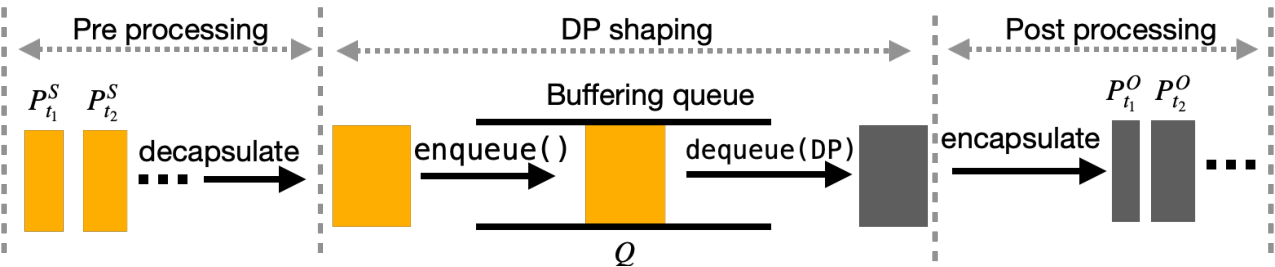
\includegraphics[width=\columnwidth]{figures/DPshaping_concept_vertical.pdf}
  %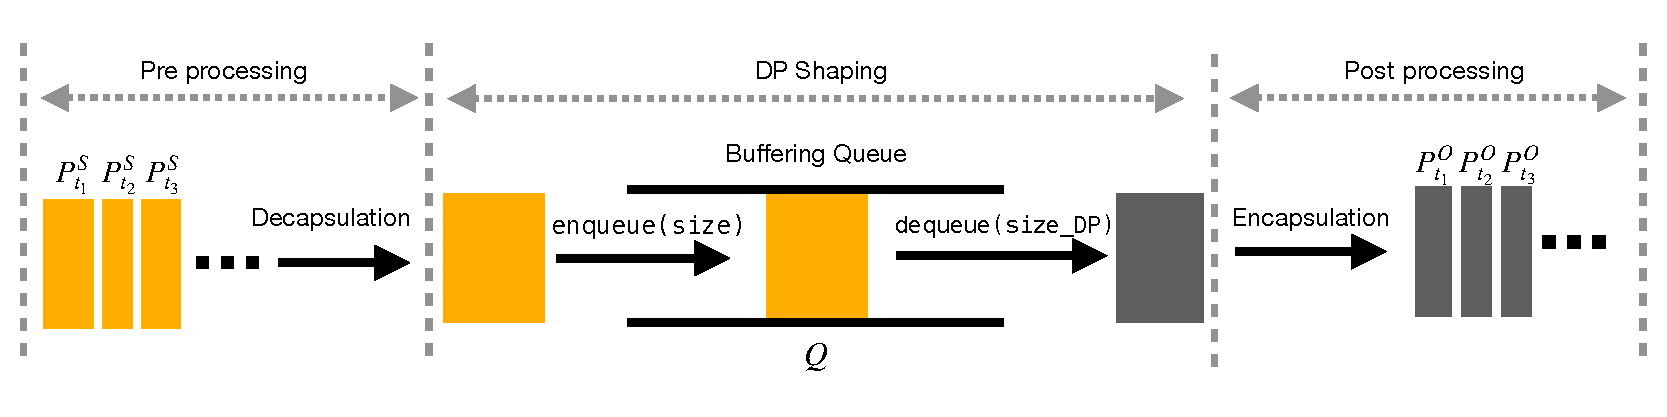
\includegraphics[width=\columnwidth]{figures/DPshaping_concept_horizontal.pdf}
  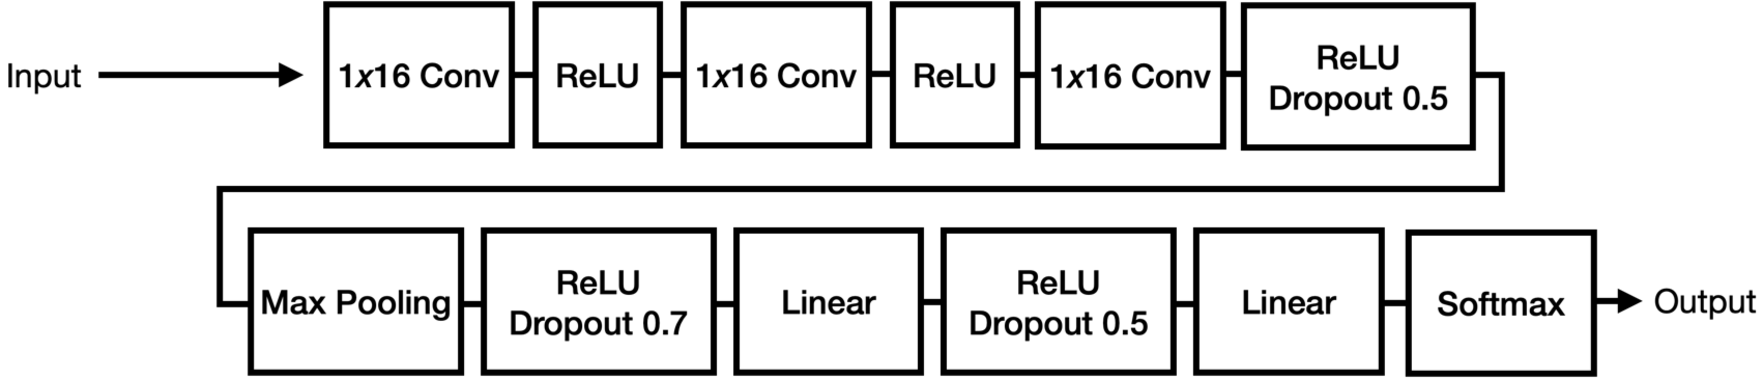
\includegraphics[width=\columnwidth]{figures/BandB_arch.pdf}
  \caption{Beauty and The Burst CNN model architecture.}
  \label{fig:bandb-arch}
\end{figure}


\subsection{TCN-based Video identification}
\todo{Move it to somewhere else to highlight that it is your contribution}
Beauty and the Burst~\cite{schuster2017beautyburst} uses a CNN-based architecture to for video identification. 
Convolutional neural networks have been shown to be effective in sequence modeling for decades~\cite{hinton1990connectionist}.
However, there are two problems with using a convolutional neural network as a sequence modeler.
First, convolutional layers applied to a sequence are not inherently causal, meaning that they look into future samples of a sequence to decide the output for the current sample.
Secondly, in contrast to recurrent neural networks(RNNs)~\cite{elman1990finding}, convolutional neural networks lack a deep effective history size of past samples in the sequence (i.e. their effective history is bounded to the number of samples that kernel can cover from the past).
To address these problems, Bai\etalc{bai2018empirical} proposed a new architecture called Temporal Convolutional Network (TCN).
The TCN utilizes a one-dimensional fully-convolutional network~\cite{long2015fully} equipped with causal dilated convolutions~\cite{oord2016wavenet}, allowing it to examine deep into the past to produce an output for the sequence at any given moment.
They added a generic residual block from input to output.
The architecture is shown in the \Cref{fig:tcn-arch}.
We evaluate the effectiveness of TCN model for network side-channel attacks in {\addref}




\begin{figure}[t]
  \centering
  %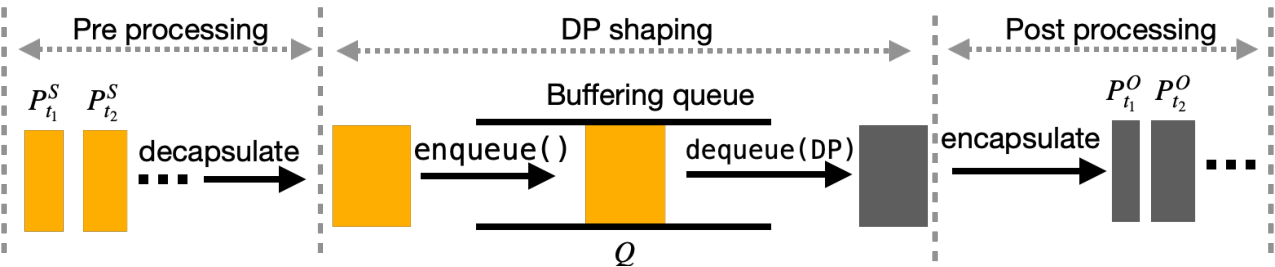
\includegraphics[width=\columnwidth]{figures/DPshaping_concept_vertical.pdf}
  %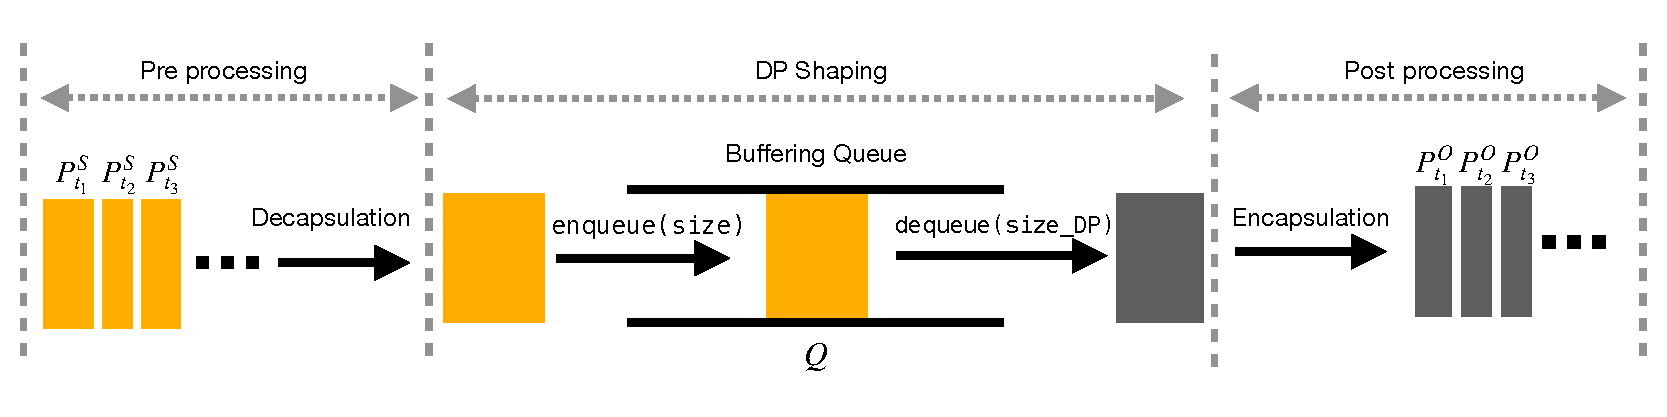
\includegraphics[width=\columnwidth]{figures/DPshaping_concept_horizontal.pdf}
  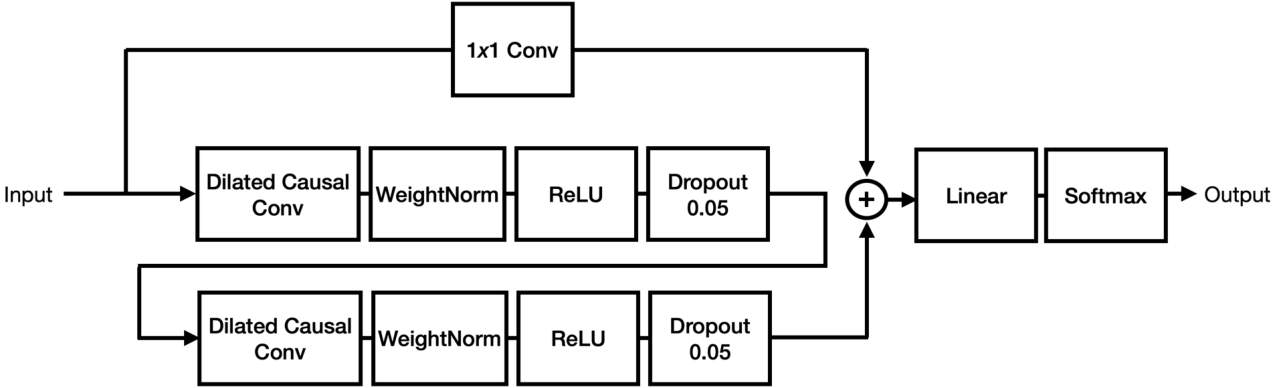
\includegraphics[width=\columnwidth]{figures/TCN_arch.pdf}
  \caption{TCN model architecture.}
  \label{fig:tcn-arch}
\end{figure}


\section{QUIC Transport Protocol}

QUIC is a modern transport layer protocol specifically developed to enhance the performance of HTTPS traffic~\cite{langley2017quic}.
In the traditional IP stack model, QUIC encompasses both the Transport layer and the Application layer.
In other words, QUIC is a user-space transport layer protocol built on top of UDP. 
Using UDP packets as the transport layer carrier allows QUIC packets to traverse current network infrastructure developed for TCP/UDP protocols such as middleboxes.
On the top of UDP, QUIC provides transport functionalities of flow control, loss recovery, encryption, and congestion control.
Unlike TCP, QUIC mitigates head-of-the-line blocking delays by introducing a novel data structuring abstraction known as streams. 
QUIC is now standardized under RFC 9000~\cite{rfc9000}, and the details of design and implementation of the protocol is well beyond the scope of this thesis.
We, however, provide a brief overview of QUIC features and functionalities that are relevant to the design of {\sys}.




\subsection{QUIC Connections}
A QUIC connection is a shared state between a client and a server.
At the initiation of each connection, a handshake phase takes place where the two endpoints engage in a cryptographic handshake protocol~\cite{rfc9001} to establish a shared secret and negotiate the application protocol.
This handshake process ensures mutual consent for communication and establishes connection parameters.

Each connection has two unique IDs, source connection ID, and destination connection ID.
By assigning each connection unique identifiers (ID), the potential changes in addressing layers at lower network levels, such as UDP and IP, do not result in incorrect packet delivery at the receiving endpoint.
Furthermore, routers can leverage existence of destination connection ID to route QUIC packets in the network to the correct endpoint.
During the handshake, one endpoint establishes the Source Connection ID by setting it in the packet header.
Similarly, the other endpoint determines the Destination Connection ID.

QUIC provides three ways to terminate a connection: idle timeout, immediate close, and stateless reset.
Each endpoint can specify an idle timeout in its transport parameters.
If the idle timeout duration elapses without any data exchange between the endpoints, the endpoint will silently close the connection (\ie without explicitly notifying the other endpoint). 
The other connection termination method is the immediate close. 
To promptly terminate the connection, an endpoint transmits \texttt{CONNECTION\_CLOSE} frame. 
This frame triggers the immediate termination of all streams within the connection.
Upon sending a \texttt{CONNECTION\_CLOSE} frame, the sender promptly terminates the connection without waiting for acknowledgment from the receiver.
A stateless reset is available as a fallback choice for an endpoint that lacks access to the connection state.
In cases of a crash or outage, it is possible for endpoints to continue sending data to an endpoint that cannot properly maintain the connection.
In such cases, the endpoint without the connection state issues the stateless reset, terminating the connection and its state machine locally.




\subsection{QUIC Streams}
QUIC's streams offer a lightweight and ordered way for applications to send byte-streams.
These streams can be either unidirectional or bidirectional, depending on the specific needs of the application.
Within a connection, each stream is identified with a new ID.
A stream ID is 62 bit integer.
Either of endpoints can create a stream just by sending data with a new stream ID. 
There are no restrictions on the number of simultaneous streams (other than, of course, the maximum number of unique IDs) or the length of each individual stream.
QUIC assigns different priorities to different streams based on the applications' requirement.
The prioritization of streams within a connection can have a substantial impact on the performance of applications.
Each stream has a dedicated header with 5 major fields: Type, Stream ID, Offset, and Data Length.
The stream header within a packet is encrypted, ensuring that adversaries are unable to discover the active streams in a connection.
Either of endpoints can terminate streams by sending a \texttt{STREAM\_RESET} frame to the other one.
In a bidirectional stream, both endpoints should send \texttt{STREAM\_RESET} message to completely terminate a stream.

% \subsection{QUIC Congestion and Flow Control}
% \subsubsection{Flow Control}
% To prevent a fast or malicious sender from overwhelming receivers' buffer, receivers must proactively limit the amount of data a sender can send.
% QUIC can perform flow control at two levels: The receiver controls the maximum amount of data the sender can send on a per-stream basis, as well as across all streams within a connection. 
% The receiver sets the initial limits for stream and connection flow controls during the handshake. 
% During the handshake, the receiver establishes the initial limits for both stream and connection flow controls. Throughout the connection, if the receiver needs to adjust the limits for a specific stream, it sends \texttt{MAX\_STREAM\_DATA} frames to the sender.
% Similarly, to change the limit for overall connection, the receiver sends \texttt{MAX\_DATA} frames to the sender.

% \subsubsection{Congestion Control}
% QUIC does not standardize any specific method of congestion control.
% Instead, it provides the necessary feedback mechanism to implement congestion control.
% The modular design of congestion control makes QUIC more flexible, allowing applications to implement a congestion mechanism that aligns with their specific requirements.
% As the default congestion control mechanism, however, QUIC uses a sender specified congestion controller similar to TCP NewReno~\cite{rfc6582}.
% Given the limitations of this thesis, a comprehensive explanation of TCP NewReno is outside its scope.
% For a more in-depth understanding of this mechanism, we kindly refer readers to the RFC, which provides detailed information and insights.


\section{Differential Privacy}\label{sec:dp-background}
% Subsection intro. Elaborate on origins of DP. Why it is useful.
Data scientists always strive to understand the general properties of a population. 
To answer questions concerning the etiology of a disease, factors contributing to a societal phenomenon, or the consequences of an economic policy, researchers collect data from individual people. They then process this data to calculate population-level statistics and propose solutions based on these aggregated statistics.
Ensuring the privacy of individuals who have contributed to these studies is of utmost importance from both ethical and legal perspectives.
In fact, the intended goal of all scientific studies is to collect valuable information about the targeted population not individual people within the population. 
However, it is impossible to learn useful information about a population while learning \textit{nothing} about individuals, leading to a paradox between usefulness of a dataset (\ie utility) and its privacy. 
Differential Privacy (DP) addresses this paradox by quantifying the extent of privacy leakage for individuals in a dataset when publishing its statistics.
Within the framework of Differential Privacy (DP), the aforementioned paradox transforms into an adjustable trade-off between the utility of data and the preservation of privacy. 

In the rest of this section, we provide the formal definition of differential privacy, highlight its main properties, and explore its potential application in the domain of traffic shaping.


%
%% 
%% Definition
%%
%


\subsection{Definitions}\label{subsec:background-dp-definitions}
A database $D$ has a fixed number of entries, where each individual data point is stored in one entry.
Following the notation proposed by Dwork \etal \cite{dwork2014algorithmic}, we represent databases by their histograms: $D \in \dbSpace$. 
In this representation, every entry $D_i$ of the database $D$ represents the number elements of type $i \in \mathcal{X}$.
\\  
Within the DP context, we define a \textit{query} as a function that operates on a database. 
Any computation performed on a database, regardless of its codomain, can be regarded as a query executed on that database.
The primary objective of differential privacy is to offer meaningful population-level information for queries executed on a database, all while protecting the privacy of individual data points within the database.
Intuitively, small changes in a database should not significantly impact the outcome of a query.
To further clarify the terms "small changes" and "significant impact", we provide definitions for neighboring databases and query function sensitivity, respectively.
\\
We measure the difference between two databases with a distance metric $\rho(D, D')$.
\begin{definition}[Neighboring databases]
  Given a distance metric $\rho$, we refer to two databases $D, D' \in \dbSpace$ as neighboring databases, if and only if $\rho(D, D') \leq 1$.             
\end{definition}
\noindent In the standard DP definition, the distance metric is simply the number of different data entries in two databases (\ie Hamming distance).
However, Chatzikokolakis \etal \cite{chatzikokolakis2013broadening} show that DP applies to a general definition of distance metrics.
\\
To quantify the extent to which a single data point can influence the outcome of a query in worst-case, we introduce the concept of sensitivity. 
\begin{definition}[$l_p$-Sensitivity]
  \label{def:norm-sensitivity}
  The $l_p$-sensitivity of a query function $f$ is:
  \begin{equation*}
    \Delta_p f = \max_{D, D'} \|f(D) - f(D')\|_p 
  \end{equation*}
where $\rho(D, D') \leq 1$ (\ie $D$ and $D'$ are neighboring databases).
\end{definition}
\noindent
Differential Privacy involves randomization of query outputs. We define a randomized algorithm as follows.
\begin{definition}[Randomized algorithm]
  \label{def:randomized-algorithm}
  A randomized algorithm $M$ with the domain $A$ and discrete range $B$, for any given $a \in A$ and $b \in B$ outputs $M(a)= b$ with probability of $(M(a))_b$.
\end{definition}

With all the necessary components in place, we are now prepared to present the formal definition of differential privacy.
\begin{definition}[Differential privacy]
  \label{def:dp}
  A randomized algorithm $M: \dbSpace \rightarrow \mathbb{R}$ is $(\varepsilon, \delta)$-differentially private if for all ${S} \subseteq Range(M)$ and for  all $D, D' \in \dbSpace$ such that $\rho(D, D') \leq 1$, we have:
  \begin{equation*}
    \Pr[M(D) \in S] \leq \exp(\varepsilon)\Pr[M(D') \in S] + \delta
  \end{equation*}
\end{definition}
\noindent
Indeed, Differential Privacy (DP) is a definition rather than a specific algorithm.
It provides a framework for ensuring privacy guarantees in various randomized algorithms. Multiple randomized algorithms can achieve $(\varepsilon, \delta)$-privacy for a given set of databases, each with different characteristics. 
Intuitively, given an output, with probability $1-\delta$ the log likelihood ratio of running the algorithm $M$ on databases $D$ and $D'$ is bounded by $\varepsilon$.
This bound ensures that the presence or absence of any individual's data in the database has a limited impact on the likelihood of obtaining a particular output.
The smaller $\varepsilon$ implies that both neighboring databases are equally likely to generate the output, resulting in more privacy.
The parameter $\varepsilon$ is commonly referred to as \textit{privacy loss} within the context of DP.
The parameter $\delta$ determines the failure probability of a differential private mechanism and is typically expected to have a small value (\ie smaller than $10^{-5}$).


%
%% 
%% Properties
%%
%

\subsection{Properties}\label{subsec:background-dp-properties}
In this section, we explore the key properties of Differential Privacy as a privacy framework.


% ROBUSTNESS TO AUXILIARY INFORMATION.
\subsubsection{Robustness to auxiliary information}
\label{subsubsec:dp-auxiliary}
The definition of Differential Privacy does not make any assumptions regarding the prior knowledge of the adversary. 
In other words, regardless of the adversary's prior knowledge, the information gained by the adversary after observing the output of a differentially private algorithm $M$ remains within the bounds specified by Differential Privacy. 
\begin{proposition}
  \label{prop:auxiliary}
  Assume that the adversary has a prior $\Pr(D)$ over the set of all possible databases $D, D' \in \dbSpace$, given the output $S$ of a $(\varepsilon, \delta)$-DP algorithm $M: \dbSpace \rightarrow \mathbb{R}$, for all $D, D' \in \dbSpace$ such that $\rho(D, D') \leq 1$, we have: 
  \begin{equation*}
    \frac{\Pr(D|S)}{\Pr(D'|S)} \leq \exp(\varepsilon) \frac{\Pr(D)}{\Pr(D')}
  \end{equation*}
\end{proposition}
In broad terms, robustness to auxiliary information in the context of Differential Privacy is similar to the security semantics of cryptographic algorithms. 
For instance, consider a scenario where an adversary possesses the knowledge that the content of an encrypted message is either a picture of a car or a picture of a tree.
In this case, observing the encrypted message does not provide any additional evidence to indicate which of the two possibilities is more likely to be the true message.
In DP, nevertheless, observing the results of private queries does change the prior knowledge of the adversary.
However, this change remains within the boundaries defined by DP and does not exceed them.

% POST-PROCESSING
\subsubsection{Post-processing}
\label{subsubsec:background-dp-postprocessing}
Differential Privacy guarantees are resilient to post-processing of the output from a DP algorithm.
In fact, in the absence of any additional knowledge, the adversary is unable to undermine the guarantees of Differential Privacy simply by processing the output of the algorithm.
\begin{proposition}
  \label{prop:post-processing}
  Consider $M: \dbSpace \rightarrow R$ as a $(\varepsilon, \delta)$-differentially private algorithm, and let $g: \mathbb{R} \rightarrow \mathbb{R}$ be an arbitrary randomized mapping, then $g(M(.)): \dbSpace \rightarrow \mathbb{R}$ is $(\varepsilon, \delta)$-differentially private. 
\end{proposition}
\noindent
This implies that regardless of the complexity of a procedure, as long as the inputs are differentially private, the output is guaranteed to maintain the same level privacy.
The post-processing property of Differential Privacy can be especially advantageous when dealing with systems that have information bottlenecks, such as situations where results from multiple calculations are aggregated at a single stage.
In such systems, by applying a differentially private algorithm to the information bottleneck, the guarantee of Differential Privacy extends to the output of the entire system. 
We specifically utilize post-processing property of Differential Privacy in the design of both the {\sys} shaping mechanism and the {\sys} middlebox. 

% PRESERVATION UNDER ADAPTIVE SEQUENTIAL COMPOSITION.
\subsubsection{Self-Composition}\label{subsubsec:background-dp-composition}
The simultaneous release of results from multiple differentially private algorithms maintains the differential privacy guarantee.
This property facilitates the modular construction of differentially private algorithms, allowing multiple DP algorithms to be combined to create more sophisticated and advanced algorithms.
Furthermore, the composition theorem enables us to compute the privacy parameters associated with the sequential release of a differentially private algorithm output, thereby facilitating multiple releases of the same DP output.
There are multiple variants of composition theorem, and we with the simplest form of composition.
\begin{proposition}[Basic composition theorem]
\label{prop:basic-composition}
  Let $M_i: \dbSpace \rightarrow \mathbb{R}$ be an $(\varepsilon_i, \delta)$-differentially private algorithm for $i \in [k]$. Then, the combination of these $k$ algorithms, $M_{[k]}: \dbSpace \rightarrow \Pi_{i=1}^{k}\mathbb{R}$ is $(\sum_{i=1}^{k}\varepsilon_i, \sum_{i=1}^{k}\delta_i)$-differentially private.  
\end{proposition}
Basic composition theorem states that the privacy loss resulting from the combination of multiple differentially private algorithms is equal to the aggregate of their individual privacy losses.
While functional, the basic composition theorem tends to overestimate the privacy loss of combined DP algorithms.
The advanced composition theorem offers a more precise and rigorous bound for the aggregated privacy loss incurred by multiple differentially private algorithms. 
\begin{proposition}[Advanced composition theorem]
\label{prop:advanced-composition}
  Let $M_i: \dbSpace \rightarrow \mathbb{R}$ be an $(\varepsilon, \delta)$-differentially private algorithm for $i \in [k]$. Then, the combination of these $k$ algorithms, $M_{[k]}: \dbSpace \rightarrow \Pi_{i=1}^{k}\mathbb{R}$ is $(\varepsilon', k\delta+\delta')$-differentially such that:
  \begin{equation*}
    \forall \delta' \geq 0: \varepsilon' = \sqrt{2k\ln(1/\delta')}\varepsilon + k\varepsilon(e^{\varepsilon} - 1)
  \end{equation*}
\end{proposition}
It is important to note that this form of composition theorem is only applicable to differentially private algorithms that share the same privacy parameters.
More sophisticated versions of the composition theorem exist, offering tighter privacy bounds~\cite{kairouz2015composition, mironov2017renyi}.
We particularly use R{\'e}nyi Differential privacy to calculate the privacy loss of our differentially private shaping mechanism.

\subsection{Mechanisms}\label{subsec:background-dp-mechanism}
\Cref{def:randomized-algorithm} provides a general definition of a randomized algorithm, while \Cref{def:dp} outlines the specific criteria that a randomized algorithm must satisfy to be considered differentially private (\ie DP mechanism).
In this section, we will explore the two most commonly used differentially private mechanisms: the Laplace mechanism and the Gaussian mechanism\cite{dwork2014algorithmic}.
\begin{definition}[Laplace Mechanism]\label{def:laplace-mechanism}
  Given any function $f: \dbSpace \rightarrow \mathbb{R}^k$ the Laplace mechanism is defined as:
  \begin{equation*}
    \mathcal{M}(x, f, \varepsilon) = f(x) + (Y_1, Y_2, \dots, Y_k)
  \end{equation*}
  where $Y_i$ are i.i.d random variables from Laplace distribution with probability density function of $Lap(\Delta_1 f/\varepsilon)$, and $\Delta_1 f$ is $l_1$-sensitivity of function $f$ (see \Cref{def:norm-sensitivity}).
\end{definition}
The Laplace mechanism is relatively easy and straightforward. 
Intuitively, it just adds a random variable driven from a Laplace distribution to the result of the query.
The variance of this random variable quantifies the privacy of query results, as a higher variance makes it more challenging for adversaries to infer the true result of the query.
\begin{proposition}
  The Laplace mechanism of \Cref{def:laplace-mechanism} is $(\varepsilon, 0)$-differentially private. 
\end{proposition}
\noindent
We omit the proof here; you can refer to the work of Dwork\etalc{dwork2014algorithmic} for a detailed proof. 
As we can see in \Cref{def:laplace-mechanism}, the failure probability of Laplace mechanism, $\delta$, is 0.
In broad terms, a mechanism can compromise failure rate $\delta$ to add less noise to query results while achieving same values for privacy loss $\varepsilon$.
\begin{definition}[Gaussian Mechanism]\label{def:gaussian-mechanism}
  Given any function $f: \dbSpace \rightarrow \mathbb{R}^k$ the Gaussian mechanism is defined as:
  \begin{equation*}
    \mathcal{M}(x, f, \varepsilon, \delta) = f(x) + (Y_1, Y_2, \dots, Y_k)
  \end{equation*}
  where $Y_i$ are i.i.d random variables from Gaussian distribution $\mathcal{N}(0, \frac{2\Delta_2 f^2}{\varepsilon^2})\ln(\frac{1.25}{\delta})$, and $\Delta_2 f$ is $l_2$-sensitivity of function $f$ (see \Cref{def:norm-sensitivity}).
\end{definition}
We particularly design our differentially private traffic shaping mechanism using Gaussian mechanism at its core. 
We elaborate on this in \Cref{subsec:dp-shaping-mechanism}.

\subsection{R\'enyi Differential Privacy}
Despite widespread usage, straightforward interpretability,, and numerous applications of standard definition of $(\varepsilon, \delta)$-differential privacy, this concept does exhibit two primary limitations. 
First, the presence of the failure probability $\delta$ in this definition contradicts the guarantee of  plausible deniability associated with differential privacy since with probability $\delta$ the secret can be completely exposed.    
Secondly, as we mentioned in \Cref{subsec:background-dp-properties}, the desirable results of strong composition theorem only holds for homogeneous DP mechanisms.
In fact, Vadhan~\etalc{murtagh2015complexity} demonstrate that the generalization of advanced composition theorem to heterogeneous DP mechanisms (\ie $(\varepsilon_i, \delta_i)$-DP for different values of $\varepsilon_i$ and $\delta_i$) is P-hard.
To address these limitations, Mironov~\etalc{mironov2017renyi} propose a new definition of differential privacy based on the R\'enyi divergence~\cite{renyi1961measures}.
R\'enyi differential privacy (RDP) is strictly stronger than $\varepsilon, \delta$-DP, meaning that any $\varepsilon, \delta$-DP mechanism is RDP though the reverse does not hold true.
In this section, we explain the core concepts of R\'enyi differential privacy (RDP), elaborate on its properties, and highlight its connection to standard definition of DP.

\begin{definition}[R\'enyi divergence]
  for two probability distributions $P$ and $Q$, the R\'enyi divergence of order $\alpha > 1$ is defined as:
  \begin{equation*}
    D_{\alpha}(P||Q) \triangleq \frac{1}{\alpha-1} \log E_{x \sim Q}\left ( \frac{P(x)}{Q(x)} \right )
  \end{equation*}
\end{definition}
R\'enyi divergence simply measure the difference between two distributions $P$ and $Q$.
For $\alpha = \infty$, the R\'enyi divergence specifically defined as:
\begin{equation*}
  D_{\infty}(P||Q) \triangleq  \sup_{x \sim Q} \; \log \left ( \frac{P(x)}{Q(x)} \right ) 
\end{equation*}
We can see that the R\'enyi divergence with $\alpha=\infty$ is closely connected to $(\varepsilon, 0)$-DP definition.
\begin{proposition}
  A randomized algorithm $M: \dbSpace \rightarrow \mathbb{R}$ is $(\varepsilon, 0)$-differentially private iff for all $D, D' \in \dbSpace$ such that $\rho(D, D') \leq 1$, we have:
  \begin{equation*}
    D_{\infty}(P||Q) \leq \varepsilon
  \end{equation*} 
\end{proposition}
\noindent Next, we provide the formal definition of R\'enyi DP.
\begin{definition}[$(\alpha, \varepsilon)$-RDP]
  A randomized algorithm $M: \dbSpace \rightarrow \mathbb{R}$ is $(\alpha, \varepsilon)$-RDP if for all $D, D' \in \dbSpace$ such that $\rho(D, D') \leq 1$, we have:
  \begin{equation*}
    D_{\alpha}(\mathcal{M}(D)||\mathcal{M}(D')) \leq \varepsilon
  \end{equation*}
\end{definition}
\noindent Indeed, all the favorable attributes of the standard definition of differential privacy, including post-processing, self-composition, and robustness to auxiliary information, remain applicable to R\'enyi differential  privacy.
Particularly, the composition theorem has a simple representation in RDP.
\begin{proposition}[R\'enyi Composition]\label{prop:rdp-composition}
  Let $M_i: \dbSpace \rightarrow \mathbb{R}$ be an $(\alpha, \varepsilon_i)$-RDP algorithm for $i \in [k]$. Then, the combination of these $k$ algorithms, $M_{[k]}: \dbSpace \rightarrow \Pi_{i=1}^{k}\mathbb{R}$ is $(\alpha, \sum_{i=1}^{k}\varepsilon_i)$-RDP.   
\end{proposition}
\noindent For an in-depth proof, we direct readers to the R\'enyi differential privacy paper~\cite{mironov2017renyi}.
So far, we explained three methods to calculate the aggregated privacy loss of multiple releases of differentially-private mechanism.
These methods are basic composition theorem, advanced combination theorem, and R\'enyi composition theorem.
The goal of these methods is to provide a tight, accurate bound on aggregated privacy loss without overestimation. 
In simpler terms, a composition theorem is superior to another, if it can provably show that the aggregated privacy loss of a differentially-private mechanism, after multiple release of results, is smaller than the aggregated privacy loss indicated by the other mechanism.
A natural question is: \textit{What is the difference between all these mechanisms?}
To answer these questions, we calculate the privacy loss reported by these mechanisms for different number of queries (\ie varying number of differentially-private releases of results).
We fix epsilon and delta per query $0.2$ and $0.0001$ respectively, and report the final privacy loss for a given number of queries.
\begin{figure}[t]
  \centering
  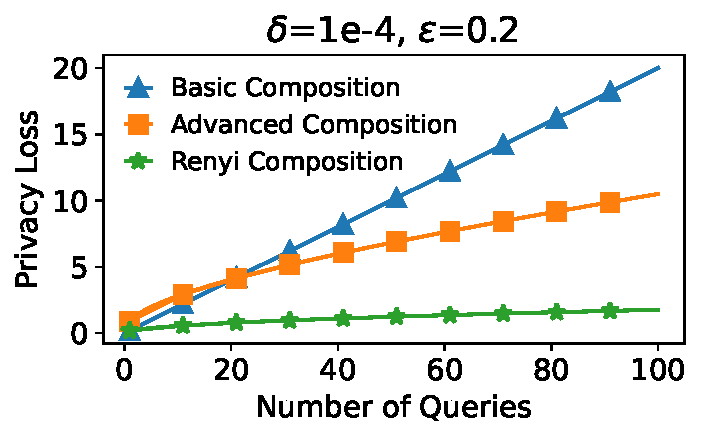
\includegraphics[width=\columnwidth]{plots/composition_comparison.pdf}
  \caption{Aggregated privacy loss of multiple queries reported by different composition methods}
  \label{fig:composition-comparison}
\end{figure}

\Cref{fig:composition-comparison} compares different methods for composing privacy loss of DP mechanisms.
We can see the effectiveness of R\'enyi methods as compared to others across all values for number of queries.
Advanced composition theorem also outperforms basic composition theorem for larger number of queries. 


As we mentioned earlier, $(\alpha, \varepsilon)$-RDP is strictly stronger than $\varepsilon, \delta$-DP. 
Next proposition shows how RDP implies standard DP.
\begin{proposition}\label{prop:rdp-better-than-dp}
  If $M: \dbSpace \rightarrow \mathbb{R}$ is an $(\alpha, \varepsilon)$-RDP mechanism, it is also $(\varepsilon + \frac{\log 1/\delta}{\alpha-1}, \delta)$-DP for any $0 < \delta < 1$. 
\end{proposition}
\noindent \Cref{prop:rdp-better-than-dp} enables us to interpret guarantees of R\'enyi differential privacy with semantics of standard differential privacy. 
Besides that, \Cref{prop:rdp-composition} provides us with the means to compose heterogeneous differentially private algorithms, while and at the end, with \Cref{prop:rdp-better-than-dp} we can still represent the final result using semantics of standard DP. 
In order to compute the privacy loss (\ie $\varepsilon$) of our differentially private shaping mechanism in \Cref{sec:dp-privacy-guarantees}, we use \Cref{prop:rdp-composition} referred to as $\textrm{DP\_compose}()$.


\section{Network Side Channel Defenses}\label{sec:ns-defenses}
% Section Intro, elaborate on the general theme of the section. 
In this section, we explore previous mitigation approaches proposed to address network side-channel attacks. 
We categorize these approaches into 4 general categories: 1- Static shaping methods, 2- Dynamic shaping methods, 3- Hybrid traffic shaping methods, 4- Adversarial traffic patterns. 




\subsection{Static Traffic Shaping}\label{subsec:static-traffic-shaping}
Static traffic shaping methods typically consist of two distinct phases: the profiling phase and the shaping phase.
During the profiling phase, the shaping mechanism collects user-specific information from the user's traffic traces.
This information can vary and may include details such as the exact traffic pattern, distribution of packet sizes, or timing of packet transmission.
The shaping mechanism then leverages this information during the shaping phase to transform users' traffic into a new pattern that ensures privacy with minimal overhead.
However, scaling static traffic shaping methods is challenging, or even impossible in many cases, due to the need for profiling numerous traffic traces.
% methods we are going to cover:
%% Walkie-Talkie 
%% Supersequence
%% Glove
%% Traffic morphing 
\subsubsection{Traffic Morphing}\label{subsubsec:traffic-morphing}
Traffic morphing~\cite{wright2009traffic} is a static approach for traffic shaping. 
In this method, the shaping mechanism alters the distribution of packet sizes in such a way that they resemble packets generated by a different website rather than the original website.
This helps to obfuscate the traffic and make it harder for eavesdroppers to associate the packets with their true source.
Traffic Morphing (TM) operates based on a technique known as \textit{Direct Target Sampling}.

First it collects the distribution of packets sizes for all websites in the dataset.
Then, Given a webpage $W$, TM randomly selects another webpage $W'$ from the dataset.
When selecting the target webpage $W'$, TM employs an optimization method to choose webpages that result in minimal overheads. 
Upon receiving each packet produced by $W$ with the size $l$, TM samples a packet size $l'$ from the distribution of $W'$. 
If $l' > l$, TM pads the outgoing packet with dummy data to match the size $l'$. 
On the other hand, if $l' < l$, TM sends $l'$ bytes and continues sampling from the distribution of $W'$ until all bytes of the original packet have been transmitted.
It is important to emphasize that the traffic morphing method does not hide the timing or duration of bursts of traffic.
Therefore, an adversary can still exploit these features of traffic traces to potentially reveal users' information based on their traffic patterns, even when traffic morphing is deployed~\cite{dyer2012peek}.


\subsubsection{Walkie-Talkie}\label{subsubsec:walkie-talkie}
Wang\etalc{wang2017walkie} propose \textit{Walkie-Talkie} as a new defense mechanism implemented in browsers to hide traffic shape of sensitive websites.
\textit{Walkie-Talkie} requires browsers modification to change the default full-duplex communication to half-duplex mode.
In full-duplex communication, multiple servers are actively transmitting web page data to the client, while the client concurrently submits additional resource requests, potentially to different servers.
In half duplex mode, on the other hand, the client only sends requests after the web servers have satisfied all previous requests.
Using half-duplex mode enables \textit{Walkie-Talkie} to change communication to a sequence of bursts of data between one client and one server at a time. 
\textit{Walkie-Talkie} represents each burst sequence $s$ as follows:
\begin{equation*}
  s = \{(b_{1+}, b_{1-}), (b_{2+}, b_{2-}), \dots \}
\end{equation*}
where $b_{i+}$ represents the size for the $i$th outgoing burst, and $b_{i-}$ represents the size for the $i$th incoming burst for sequence $s$.
\\
For any sensitive website $W$, \textit{Walkie-Talkie} first extract the burst sequence $s$.  
Then, using a similar approach to Traffic Morphing~\cite{wright2009traffic}, \textit{Walkie-Talkie} chooses a decoy website $W'$ with burst sequence of $s'$.
At the transmission time, \textit{Walkie-Talkie} reshapes the burst sequence of $s$ to sequence $\hat{s}$ such that:
\begin{equation*}
  (\hat{b}_{i+}, \hat{b}_{i-}) = (\max(b_{i+}, b_{i+}'), \max(b_{i-}, b_{i-}'))
\end{equation*}
where $\hat{b}_{i+}$, $b_{i+}$, and $b_{i+}'$ represent the size for the $i$th outgoing burst in sequences of shaped traffic $\hat{s}$, original webpage $s$, and decoy webpage $s'$ respectively.
The same notation used for incoming burst sizes.
Therefore, if an adversary observes the sequence $\hat{s}$, it can not ascertain whether the users accessed $W$ or $W'$.
Choosing multiple decoy burst sequences for any sensitive can further increase the privacy of \textit{Walkie-Talkie}.

Essentially, \textit{Walkie-Talkie} use as a clustering technique for shaping traffic, conceptually similar to Supersequence~\cite{wang2014supersequence}, Glove~\cite{nithyanand2014glove}, and Tamaraw~\cite{cai2014systematic}.
It maps the traffic shapes of various web pages to the same pattern, effectively rendering them indistinguishable for potential adversaries.
The advantages of the \textit{Walkie-Talkie} are: it adds small overheads compared to other defenses, requires minimal computation to extract the burst sequence of shaped traffic, and stores small metadata to for decoy webpages.
On the other hand, it had several disadvantages. 
First, \textit{Walkie-Talkie} requires browser modification.  
Secondly, similar to most of the static traffic shaping methods, \textit{Walkie-Talkie} should identify the burst sequence of a webpage before its transmission.
Finally, the adoption of half-duplex mode in browsers imposes a notable constraint on the scalability of this approach, as numerous applications, such as video streaming and file downloading, require multiple and simultaneous communications with web servers.


% ---------------------------------------------------% 
% ---------------------------------------------------% 
% ---------------------------------------------------% 
% ---------------------------------------------------% 
% ---------------------------------------------------% 

\subsection{Dynamic Traffic Shaping}\label{subsec:dynamic-traffic-shaping}
In these methods, the traffic shaping defense mechanism does not require prior profiling of application traffic traces in order to perform its function.  
In other words, the shaping mechanism determines the shape of outgoing traffic at the transmission time.
These methods are typically more practical compared to static approaches, as it can be challenging to profile all possible traffic patterns for sophisticated network applications.
On the other hand, ad-hoc decisions regarding the shaping of traffic at the time of transmission can potentially result in information leakage.
In this section, we provide an overview of dynamic traffic shaping methods, highlight their unique characteristics, and discuss their strengths and weaknesses.

\subsubsection{WTF-PAD}\label{subsubsec:wtf-pad}
WTF-PAD~\cite{juarez2016toward} is a simple generalization of Adaptive Padding (AP)~\cite{shmatikov2006timing} method to be used in Tor~\cite{dingledine2004tor}. 
The core shaping mechanism in this method is the same as adaptive padding. 
In this method, traffic shaping works based on a state machine with three states: \textit{Wait}, \textit{Burst}, and \textit{Gap}. 
The shaping procedure starts in \textit{Wait} state. 
Upon receiving a packet, shaping mechanism state changes to \textit{Burst} mode. 
WTF-PAD measures the inter-arrival time of the next packets. 
If the inter-arrival time is less than a threshold defined in algorithm, it remains in \textit{Burst} state. Otherwise, the states changes to \textit{Gap}.
In \textit{Gap} state, WTF-PAD samples a random variable from a distribution of inter-arrival times for packets during traffic burst.
This sampled random variable serves as a timer, determining the interval at which the next dummy packet should be transmitted.
When an application sends a packet, the shaping mechanism transitions to the \textit{Burst} state. Otherwise, the mechanism remains in the \textit{Gap} state, continuing to send dummy packets at random intervals. 

Although WTF-PAD pad has zero latency overhead and moderate bandwidth overheads, it provides no formal privacy guarantees.
In fact, multiple new traffic analysis attacks are able to extract users information from their traffic pattern while WTF-PAD is deployed.
\todo{Add the references and also mention attacks that are successful against WTF-PAD}.


\subsubsection{BuFLO and CS-BuFLO}\label{subsubsec:buflo}
Dyer et al.~\cite{dyer2012peek} conducted a comprehensive study on network side-channel attacks and state-of-the-art defense mechanisms available at the time, providing valuable insights into this field. 
Their negative results showed that none of the countermeasures at the time could completely mitigate network side-channel attacks.
To address this problem, they proposed a shaping mechanism known as Buffered Fixed-Length Obfuscator (BuFLO).
BuFLO can be considered as a relaxation of the constant shaping method.
For every given webpage $W$, BuFLO sends fixed-sized packets at constant intervals for a specific duration of time.
We represent packet sizes with $p$, packet frequency with $f$, and the sending duration with $T$. 
If the packet sequence of webpage $W$ takes longer than the specified time $T$, BuFLO continues sending fixed-sized packets at fixed intervals until transmission is finished, revealing the duration of the flow. 
When all flows have durations shorter than $T$, BuFLO effectively operates similarly to constant shaping.
In such cases, BuFLO inherits the advantages and disadvantages associated with the constant shaping method.
\todo{Add the references and also mention attacks that are successful against WTF-PAD}.

To address problems associated with BuFLO, Cai~\etal~\cite{cai2014cs} proposed Congestion Sensitive Buffered Fixed-Length Obfuscator (CS-BuFLO).
CS-BuFLO enhances the BuFLO traffic shaping method by applying it bidirectionally, encompassing both the client-to-server and server-to-client directions. 
To optimize network latency and reduce network load, CS-BuFLO dynamically adjusts the frequency of packets at the server side based on the client's transmission rate.
Additionally, to address the issue of fixed transmission durations, CS-BuFLO rounds page sizes to the nearest power of two. 
Overall, CS-BuFLO is a more pragmatic approach to perform traffic shaping compared to BuFLO. 
However, it is important to note that both the transmission rate adjustment and the padding to powers of two in CS-BuFLO have the potential to leak information.
The authors of CS-BuFLO, however, do not provide a quantification of the extent of information leakage resulting from these mechanisms


\subsubsection{Tamaraw}\label{subsubsec:tamaraw}
Cai et al.~\cite{cai2014systematic} conducted a systematic study on network side-channel defenses, proposing a novel notion for privacy in defense mechanisms.
Additionally, they developed a network side-channel defense based on BuFLO~\cite{dyer2012peek} called Tamaraw. 
We first overview their notion of privacy, and then, discuss Tamaraw defense mechanism.


Tamaraw \cite{cai2014tamaraw} provides a
mathematical notion of privacy guarantee of a shaping strategy, called $\epsilon$-security.
To disambiguate with {\sys}'s notion of $(\varepsilon, \delta)$-DP, we rename Tamaraw's $\epsilon$ variable with $\gamma$ in this section.
We show that $(\varepsilon, \delta_{\winlen})$-DP definition is strictly stronger than Tamaraw's $\gamma$-security definition.
We start by explaining Tamaraw's definition.
\\
\noindent
Tamaraw defines $W$ as the random variable that represents the label of a
traffic trace.
For each traffic trace, $w$, let $T_{w}$ $T_{w}^{D}$ be the random variables representing
the packet trace of $w$ before and after applying shaping on $w$ respectively.
The distribution of $T_{w}^D$ encompasses all variations in observed
patterns of a trace $w$ resulting from both the defense mechanism and the
network, and the distribution of $T_{w}$ only captures the randomness added in the network.
The attacker can measure the distribution of $W$ and $T_{w}^{D}$ independently.
\\
\noindent
Upon observing a trace $t$ on the network, an optimal attack $A$, selects the
label that corresponds to the maximum likelihood of observing that trace.
\begin{equation*}
  A(t) = \argmax_{w}{\Pr[W=w]\Pr[T_{w}^{D}=t]}
\end{equation*}
For any attack $A$, we represent the probability that attack output the label $w_i$ with $\Pr_A[w_i]$.
\begin{definition}[Tamaraw $\gamma$-privacy]
  A fingerprinting defense $D$ is said to be uniformly $\gamma$-private if for the attack $\mathcal{A}$ if we have:
  \begin{equation*}
    \max_w\big[\Pr[A(T_w^D)=w]\big] \leq \gamma
  \end{equation*}
\end{definition}

\begin{proposition}
  Tamaraw $\gamma$-privacy is strictly weaker than the notion of $(\varepsilon, 0)$-differential privacy.
\end{proposition}
\noindent
To prove the above proposition, we need to prove the following two lemmas.

\begin{lemma-numbered}
  There exists a Tamaraw $\gamma$-private defense mechanism that fails to satisfy $(\varepsilon, 0)$-differential privacy for any given value of $\varepsilon$.
\end{lemma-numbered}
\begin{proof}
%  Assume a closed-world setup of $n$ webpages.
    Consider a web service with a dataset of $n$ web pages.
    We propose the following defense mechanism, $D$, with two parameters $\alpha$ and $\beta$:
    \begin{enumerate}
    \item For the webpage $w_i: i=j$, $D$ reshapes it to the constant-rate pattern, $O_c$, with probability $\beta$. Otherwise, with probability $1-\beta$, it reveals the original traffic pattern of the webpage, $T_{w_{i=j}}$.
    \item For any webpage $w_i: i \in \{1, 2, \dots, j-1, j+1, \dots, n\}$, $D$ reshapes it to the constant-rate pattern, $O_c$, with probability $\alpha$ such that $\alpha > {e^{\varepsilon}}\beta$. Otherwise, $D$ reveals the original pattern of $w_i$, $T_{w_{i\neq j}}$, with probability $\alpha$.
    \end{enumerate}
    The probability that any attack can correctly identify the label for webpage $w_j$ is upper-bounded by:

    \begin{align*}
      & \Pr[A(T^{D}_{w_{i=j}}) = w_j]
      \\
      & = \Pr[A(T^D_{w_{i=j}}) = w_j | T^D_{w_{i=j}}=T_{w_{i=j}}]\Pr[T^D_{w_{i=j}}=T_{w_{i=j}}] +
      \\
      &~~~~\Pr[A(T^D_{w_{i=j}}) = w_j | T^D_{w_{i=j}}=O_c]\Pr[T^D_{w_{i=j}}=O_c]
      \\
      & \leq  1.(1-\beta) + \frac{1}{n}\beta = p_c^j
    \end{align*}
    For $(1- \frac{n\gamma - 1}{n-1}) < \beta$ we have: $p_c^j \leq \gamma$.
    \\
    Similarly, the probability that any attack can correctly classify $w_{i\neq j}$ is upper-bounded by $p_c^i = 1-\alpha + \frac{\alpha}{n}$, and for $(1- \frac{n\gamma - 1}{n-1}) < \alpha$ we have: $p_c^j \leq \gamma$.
    Therefore, for all values of $\alpha$ and $\beta$ such that $(1- \frac{n\gamma -
    1}{n-1}) < \beta < \alpha$, the probability that any attack can successfully
    guess victim traffic stream in both cases is less than $\gamma$, and
    the defense is uniformly $\gamma$-private.
    \\
    When the output of the algorithm is a constant pattern, $O_{c}$, with the probability $\beta$ the original webpage is $j$, and with probability $\alpha$, it can be any other webpages. Thus, we have:
    \begin{equation*}
    \log(\frac{\Pr[T_{w_{i\neq j}}^{D}=O_{c}]}{\Pr[T_{w_{i=j}}^{D}=O_{c}]})
    = \log(\frac{\alpha}{\beta}) > \varepsilon
    \end{equation*}
  Therefore, it fails to guarantee $\varepsilon$-differential privacy.
\end{proof}


\begin{lemma-numbered}
  A $(\varepsilon, 0)$-differentially private shaping algorithm is Tamaraw $\gamma$-private for:
  \begin{equation*}
    \varepsilon \leq \log(n\gamma)
  \end{equation*}
\end{lemma-numbered}
\begin{proof}
  For a given trace, $w$, the random variable $T_{w}^{DP}$ represents packet
  trace of $w$ after  a differentially private shaping mechanism is applied.
  \\
  The classification attack on shaped traffic analysis the shaped traces so it can be considered as post-processing of the results of a
  differentially private shaping mechanism (i.e. defense), and is differentially
  private. Therefore,
  we have:
  \begin{align*}
    \frac{\Pr[A(T_{w_{i}}^{DP}) = w_i]}{\Pr[A(T_{w_{j}}^{DP}) = w_i]} \leq e^
    {\varepsilon}
    \\
    \rightarrow \Pr[A(T_{w_{i}}^{DP}) = w_i] \leq e^
    {\varepsilon} .\Pr[A(T_{w_{j}}^{DP}) = w_i]
  \end{align*}
  Intuitively, this implies that the likelihood of the attacker correctly classifying the trace with label $i$ compared to incorrectly classifying it with label $j$ is bounded by $e^{\varepsilon}$.
  The above inequality is correct for all $w_j: j\in \{1, 2, \dots, n\}$, therefore we can calculate the summation over $j$.
  Extending the above equation we have:
  \begin{align*}
    n\times \Pr[A(T_{w_{i}}^{DP}) = w_i] \leq e^{\varepsilon}\sum_{j=1}^{n} \Pr[A(T_{w_{j}}^{DP}) = w_i] \\
    = e^{\varepsilon} \operatorname{Pr}_{A}[w_i]
  \end{align*}
  where $\Pr_{A}[w_i]$ is the probability that attack $A$ outputs the label
  $w_i$.
  Therefore, for any given trace $w_i$, the probability that any attack $A$, classifies it correctly is bounded by:
  \begin{equation*}
    \Pr[A(T_{w_{i}}^{DP}) = w_i] \leq \frac{e^{\varepsilon} \Pr_{A}[w_i]}{n}
  \end{equation*}
  Therefore, the probability that an attacker can guess the victim’s trace is bounded by:
  \begin{align*}
    \max_{w_i}{\Pr[A(T_{w_{i}}^{DP}) = w_i]} \leq \frac{e^{\varepsilon}}{n} \max_{w_i}{\operatorname{Pr}_{A}[w_i]} \leq \frac{e^{\varepsilon}}{n} \leq \gamma
  \end{align*}
\end{proof}
Putting the two lemmas together, we prove that the notion of differential
privacy is strictly stronger than Tamaraw's.

Tamaraw's shaping method is almost the same as BuFLO~\cite{dyer2012peek}. The only difference it that instead of padding the total transmission time a threshold $T$, Tamaraw pads the total number of packets to multiples of a padding parameter $L$.
In other words, if the total packet number for a webpage $W$ is $n_W$, Tamaraw pads it to a size of $\lceil \frac{n_W}{L} \rceil \times L$.
As the value of $L$ increases, Tamaraw offers enhanced privacy; however, this also results in higher overheads.




\subsection{Adversarial Traffic Patterns}

\subsection{Traffic Shaping Frameworks}
\subsubsection{QCSD}









\chapter{Differentially-Private Traffic Shaping}
\label{ch:dp-shaping}
% Chapter Introduction
% Traffic shaping can be implemented at different layers within the network stack of an application.
% At the transport layer, shaping involves dynamically adjusting the data transmission rate, specifically the size of data transmitted within a given time window, to ensure that the size and timing of data transmission do not disclose sensitive information of the applications.
% At the network layer, traffic shaping is about transmitting packets in a manner that does not reveal users' private information through the timing and sizing of the packets. 
% The selection of either approach has profound implications for both the design of shaping algorithm and the traffic shaping system itself.
% Designing traffic shaping mechanism at network layer requires determining the size and transmission of every individual packets. 
% Networking hardware capabilities, such as popular NICs, and network protocol specifications significantly constrain the design space in this context~\cite{mehta2022pacer}.  
% On the other hand, to design a traffic shaping mechanism that operates on the top of transport layer, it is crucial to assume that \textit{after traffic shaping, the shaped traffic remains unaffected by the content or pattern of the unshaped traffic, during all subsequent processes such as encryption, packetization, and packet transmission scheduling}.
% This assumption guarantees that the shaping mechanism maintains its integrity and effectively separates the sensitive information from the traffic pattern regardless the way network stack transmits the shaped traffic.
% {\sys} performs differentially-private traffic shaping on the top of transport layer, and in section {\addref} we elaborate on how our system satisfies this assumption.
 

The objective of our DP traffic shaping is to dynamically adapt the data transmission rate based on the available data stream, while simultaneously ensuring that the DP guarantees remain intact for any information that an attacker can observe, as specified in our threat model (See \Cref{sec:threat-model}).
The design of our traffic shaping algorithm relies on three key steps.
%
First, in \Cref{sec:dp-shaping-definitions}, we formalize the information available to an attacker observing an application stream, which is all information such as packet sizes or timing at the finest granularity of observation.
We propose to use a buffering queue to collapse all this information into a sufficient statistic to adapt {\sys}'s transmission rate: the size of data in the queue waiting to be transmitted through our shaping mechanism.
%
Second, in \Cref{subsec:dp-shaping-mechanism}, we show how to perform {\em DP measurements} of our buffering queue, to adapt \sys's transmission rate with DP guarantees.
We show that during data transmission with {\sys} shaping mechanism, the change of queue size is bounded, allowing us to perform DP measurements.
%
Third, we describe our mechanism for sending data based on DP measurements, which completes our DP shaping mechanism in \Cref{sec:dp-privacy-guarantees}.
Intuitively, we can use DP queue measurements and public information such as network conditions to decide the amount of data to transmit.
Transmissions contain applications' queued data when some is available and dummy data otherwise.
The traffic pattern observed by the attacker is a post-processing of the DP queries issued on the queue (depending only on the private information obtained through the DP measurements) and is differentially-private.


\section{Definitions and Assumptions}
\label{sec:dp-shaping-definitions}
An application's stream can be represented as a sequence of packets:
\begin{equation}
    \istream = \{{P^S_1}, {P^S_2}, {P^S_3}, \dots \}
\end{equation}
where ${P_i}^S = (l^S_i, t^S_i)$ indicates that the $i$\textsuperscript{th} input packet in $S$ has length $l_i^S$ bytes and is transmitted at timestamp $t_i^S$.
Without shaping, an adversary can precisely observe $\istream$ and infer the content, which is correlated with the~stream~\cite{schuster2017beautyburst}.

Our DP shaping relies on two key ideas.
First,~it models the DP guarantees for the (potentially long) traffic streams in windows of fixed length $\winlen$, denoted by \mbox{($\varepsilon_{\winlen}, \delta_{\winlen}$)-DP}.
An input sequence over window $j$ is a finite~sub\-sequence $S_{j} \subset S$, such that $S_{j} = \{ P^S_i~|~P^S_i \in S~and~t_i \in j \}$.
{\sys}'s DP guarantees cover all (overlapping) windows up to size $\winlen$.
A key assumption for {\sys}'s DP guarantees to hold over $\winlen$-sized windows is that the tunnel can always transmit all incoming data from application streams within any $\winlen$-sized time window.
In other words, we assume:
\begin{assumption}\label{assumption:window}
  All bytes enqueued prior to or at time $t$ are transmitted by time
  $t+W$.
\end{assumption}
We explain how to realize this assumption in a tunnel design in \Cref{ch:design}.
Under this assumption, the privacy loss of the complete traffic stream is simply a DP composition of the privacy losses over consecutive windows.
The window length $\winlen$ is a configuration parameter, which is set before the start of an application's transmission. In practice, $\winlen$ would be on the order of a few seconds.

Secondly, we use the primitive of a {\em buffering queue} to control the maximum information accessible by an adversary within each window.
We denote the number of bytes present in the queue (\ie length of the queue) by $\qlen$.
Conceptually, {\sys} extracts bytes from the input stream, $\istream$, and enqueues them.
Furthermore, we discretize time into $\winlen$-sized windows and, at the beginning of each time window, {\sys} adds DP noise to the queue length to determine the amount of data from the queue that should be transmitted as shaped traffic.
The shaped traffic is then transmitted as a packet sequence denoted by $\ostream$, which is observable by an adversary.
\begin{equation}
    \ostream = \{{P^O_1}, {P^O_2}, {P^O_3} \dots \}
\end{equation}
While shaping requires discretizing transmit windows, the DP guarantees apply over arbitrary windows.

In the rest of this section, we focus on {\sys}'s DP guarantees over a single window.
We first formally define a notion of ($\varepsilon_\winlen$,$\delta_\winlen$)-DP privacy, which guarantees DP over transmission windows of length $\winlen$.
The guarantee applies over all $\winlen$ windows, and applying DP composition yields guarantees over multiple windows.
Then, we provide an overview of the DP shaping mechanism, which further samples noise in multiple shorter uniform intervals within each window.
Finally, we prove that the shaping mechanism provides ($\varepsilon_\winlen$,$\delta_\winlen$)-DP.
To formalize {\sys}'s DP guarantees, we first define a meaningful distance between any pair of streams in windows of length $\winlen$ and the associated neighboring definition:

\begin{definition}
Two streams $S_{j}$ and $S_{j}'$, transmitted in a window $j$,
are neighbors
%    if, within each time window $\window$,
if their L1-norm distance is at most~$\ssens$ bytes in a window of upto length $\winlen$, \ie ${\norm{~S_{j} - S_{j}'~}}_1 \leq \ssens$.
\label{def:neighboring-streams}
\end{definition}

$\ssens$ is the max L1-norm distance between each pair of application streams transmitted in any window $j$.
We utilize the L1-norm (the sum of absolute values) as our distance metric to quantify the dissimilarity between two traffic streams, as it captures differences in both packet sizes and temporal pattern.


\section{The Shaping Mechanism}
\label{subsec:dp-shaping-mechanism}
\paragraph{From windows to intervals.}
Based on \Cref{assumption:window} and \Cref{def:neighboring-streams}, the window length $\winlen$ affects the maximum number of bytes that can be accumulated in the buffering queue (thus, the maximum distance between stream pairs), as well as the transmission delay of the payload bytes enqueued.
Specifically, large windows lead to high-latency, bursty traffic.
To reduce latency and burstiness, {\sys} further splits windows into smaller intervals of length $\dpintvl$ and samples noise at the beginning of each interval.
In absence of shaping, the queue length corresponds to the amount of unshaped traffic transmitted in an interval of $\dpintvl$.
The privacy loss over a window is now defined by applying DP composition on the privacy loss of individual intervals.

To apply noise in each interval, we now define the sensitivity of the queue  length over intervals of length $\dpintvl$.
Sensitivity, denoted $\qsens$, is the maximum difference in the queue length over any interval $\dpintvl$ that can be caused by changing one application stream to another.
Formally, consider two alternative streams $\streamw{j}$ and $\streamw{j}'$ passing through the queue.
Suppose that when transmitting $\streamw{j}$ (similarly $\streamw{j}'$), the queue length at the beginning of its $k$\textsuperscript{th} interval is denoted by $\qlent{k}$ (respectively $\qlent{k}'$). Then:
\begin{equation}
    \qsens = \max_{k = 0}^{\numupdates}~\max_{\streamw{j},
        \streamw{j}'} | \qlent{k} - \qlent{k}' |
    \label{eqn:ssens}
\end{equation}


\begin{figure}[t]
    \centering
    %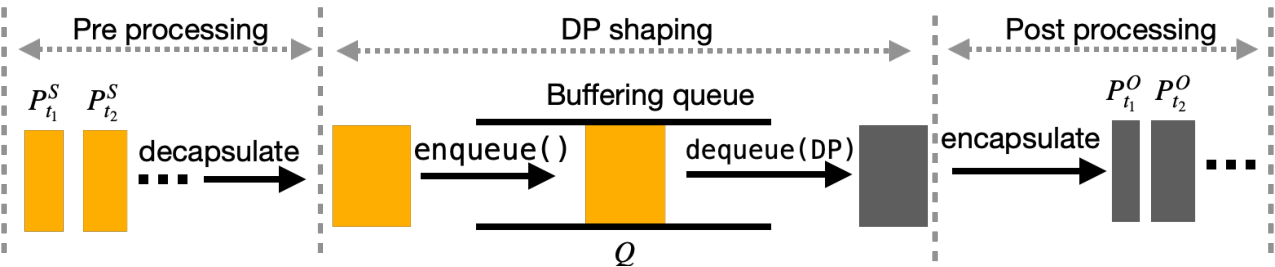
\includegraphics[width=\columnwidth]{figures/DPshaping_concept_vertical.pdf}
    %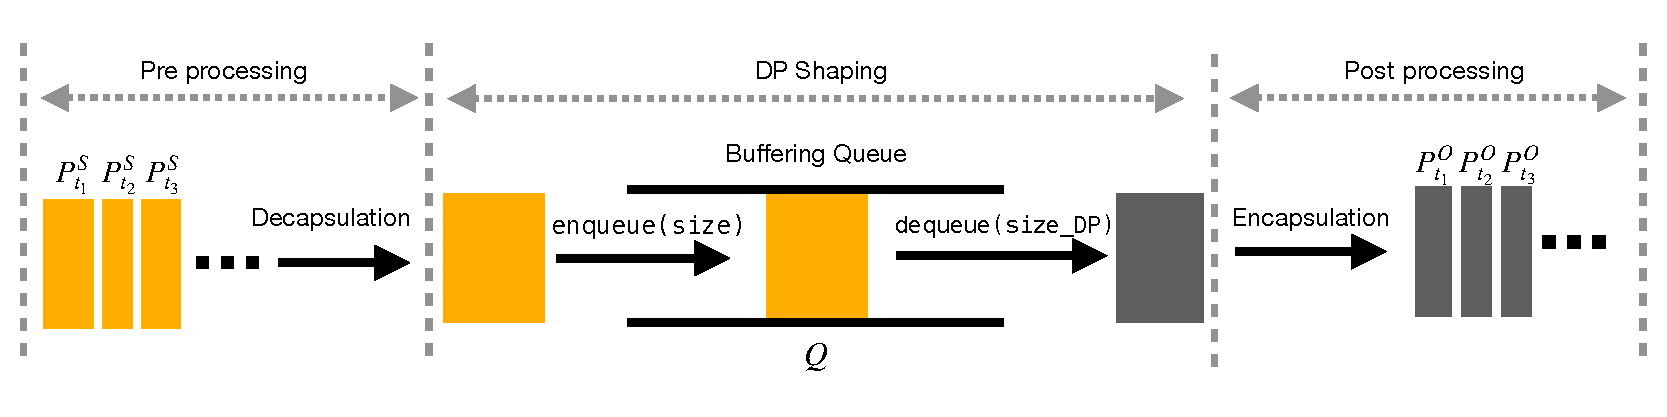
\includegraphics[width=\columnwidth]{figures/DPshaping_concept_horizontal.pdf}
    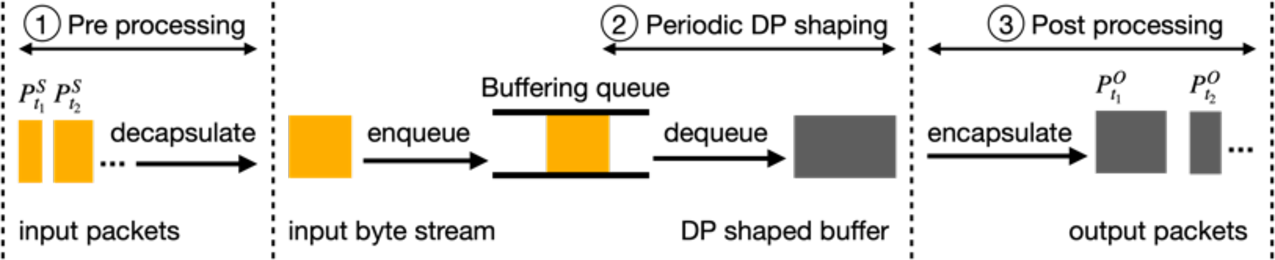
\includegraphics[width=\columnwidth]{figures/dp-overview.pdf}
    \caption{Overview of DP shaping}
    \label{fig:dp-overview}
\end{figure}

\paragraph{Shaping overview.}
\sys's DP shaping involves three steps as shown in \Cref{fig:dp-overview}.
\begin{enumerate}
    \item As application packets arrive in a window $\window$, the preprocessing step extracts the payload bytes and enqueues them into the buffering queue.
    \item In a periodic interval $k$, the core DP shaping algorithm performs a DP measurement, which entails sampling noise $z$ from a DP distribution and computing a DP burst size $\qlendpt{k} \triangleq \qlent{k} + z$.
    The shaping logic then prepares a {\em shaped buffer} of length $\qlendpt{k}$ with the application bytes available in the queue and dummy bytes if required.
    The DP shaping logic uses an additive Gaussian noise mechanism.
    The noise $z$ is sampled from a normal distribution $\mathcal{N}\big(\mu,~\sigma^2\big)$ parameterized by $\epsilon_\dpintvl$, $\delta_\dpintvl$, and~$\qsens$:
    The mean $\mu$ is 0 and the variance $\sigma^2$ is given by $\frac{2\qsens^2}{\varepsilon_\dpintvl^2}\ln(\frac{1.25}{\delta_\dpintvl})$.
    If the sampled noise is negative, we retain some of the data in the queue until the next DP measurement interval.
    Given this noise distribution, one measurement is \mbox{$(\epsilon_\dpintvl, \delta_\dpintvl)$-DP}.
    \item Data in the shaped buffer is then split into one or more packets and transmitted to the network. Since these packets are a post-processing of the DP-shaped buffer, they preserve DP as long as no new dependency on private data is introduced. 
    This last constraint requires the packets' size and transmit time to be selected independently of the data.
    We describe how {\sys} enforces this constraint in \Cref{ch:design}.
\end{enumerate}
The privacy loss ($\varepsilon_{\winlen}$) and bandwidth overheads of the DP shaping (represented by $\sigma_\dpintvl$, \ie the standard deviation of the noise distribution function) depend on $\winlen$, $\ssens$, and the number of intervals $\varnumupdates = \numupdates$ in $\winlen$.
Additionally, the latency overheads depend on $\dpintvl$.
Note that for a specific value of $\ssens$ and $\varnumupdates$, the DP guarantee $\varepsilon_{\winlen}$ is fully specified by $\sigma_\dpintvl$, and remains the same even at different time scales.
That is, scaling $\winlen$ and $\dpintvl$ proportionally does not change the privacy and overhead costs.
We analyze the impact of different choices for these parameters on the privacy guarantees and overheads in \Cref{sec:eval-privacy-params}.
Here, we focus on a formal model of the DP guarantees.

\section{Privacy Guarantees}
\label{sec:dp-privacy-guarantees}
At a high level, analyzing the  ($\varepsilon_{\winlen}, \delta_{\winlen}$)-DP guarantee of the overall shaping mechanism requires two steps:
\begin{enumerate}
    \item Showing that the difference in the buffering queue length is bounded for neighboring streams for all transmissions of the streams (\Cref{prop:sensitivity}).
    \item Composing the DP cost of each measurement over the intervals defining a window of length $\winlen$ (\Cref{prop:dp}).
\end{enumerate} 
We first show that the sensitivity of each measurement $\qsens$ is at most the window sensitivity $\ssens$:
\begin{proposition}\label{prop:sensitivity}
    {$\sys$} enforces $\qsens \leq \ssens$.
\end{proposition}
\noindent To prove the proposition stated above, we will first establish the following lemma.
\begin{lemma}
    Assume two neighboring traffic streams, $\streamw{j}$ and $\streamw{j}'$
    ($\|\streamw{j}-\streamw{j}'\|_1 \leq \ssens$), transmitted through {\sys}.
    If both streams are reshaped to the same output stream, $\ostream$, then by
    the end of any interval of shaping execution, the length of the buffering queue
    for the first and second streams are $\ssens$-close.
    In other words we have:
    
    \begin{equation}\label{equ:composition}
            \forall k \geq 0 : |\qlent{k} - \qlent{k}'| \leq \ssens
    \end{equation}
\end{lemma}

\begin{proof}
    {\sys} dequeues data from the buffering queue periodically at intervals of $T$
    seconds.
    Thus, while transmitting a stream $\istream$, the length of the buffering queue
    at the end of $k$\textsuperscript{th} interval, $\dpintvl_{k}$ is a function of
    three variables:
    \begin{enumerate}
            \item The length of the buffering queue at the end of
            $(k-1)$\textsuperscript{th} interval, $\qlent{k-1}$.
            \item The total number of payload bytes that have been dequeued from the
            buffering queue in the $k$\textsuperscript{th} interval,
            ${\payload}_{k}$.
            \item The number of new payload bytes from the application stream added
            to the buffering queue since the previous interval, which is the sum of
            sizes of all packets arriving between $(k-1)$\textsuperscript{th} and
            $k$\textsuperscript{th} interval, \ie
    %        $\sum_{T_{k-1} \leq t < T_k} P^S_t$
            $\sum_{\dpintvl_{k-1} \leq t < \dpintvl_{k}} P^S_t$.
    \end{enumerate}
    As two streams are reshaped to the output stream, $\ostream$, the DP burst size for two streams is the same in all intervals (i.e. $\forall k \geq 0 : \qlendpt{k} = \qlendpt{k}'$).
    
    Therefore, the length of the buffering queue after dequeue in the
    $k$\textsuperscript{th} interval is given by:
    \begin{equation}
    \qlent{k} =
    {\qlent{k-1}}
    +
    {\sum_{\dpintvl_{k-1} \leq t < \dpintvl_{k}} P^S_t}
    %{\sum_{T_{k-1} \leq t < T_k} P^S_t}
    -
    {{\payload}_{k}}
    \label{equ:queue-state}
    \end{equation}
    %\\
    Based on \Cref{equ:queue-state}, the difference between queue lengths of two
    neighboring streams, $\streamw{j}, \streamw{j}'$ at $k^{th}$ interval is:
    \begin{align}\label{equ:queue_state_expansion}
    & \qlent{k} - \qlent{k}'~=~(\qlent{k-1} - \qlent{k-1}')~+\\
    \nonumber
    & (\sum_{\dpintvl_{k-1} \leq t < \dpintvl_{k}}P^S_t - \sum_{\dpintvl{k-1} \leq t < \dpintvl_{k}}P^{S'}_t)
    -
    ({\payload}_{k} - {\payload}_{k}')
    \end{align}
    We divide the proof into two different steps.
    First, we show that the dequeue stage of the shaping mechanism does not increase the difference in queue lengths.
    Secondly, we show that under \Cref{assumption:window}, the enqueue stage of incoming streams does not increase the difference in queue lengths beyond $\ssens$.
    
    Suppose $\streamw{j}$ and $\streamw{j}'$ are reshaped to the same output stream,
    $\ostream$. Thus, the sizes of output packets generated in each decision
    interval $\dpintvl$ when transmitting either streams is the same. However, the
    content of the output packets in each stream might differ based on the sizes and
    timing of the packets in each input stream.
    For the shaping mechanism, this implies that the number of payload bytes
    dequeued from the buffering queue when transmitting each stream might not
    necessarily match.
    %This is because one queue might not have a sufficient amount of traffic to meet
    %the requirements of the DP decision, resulting in the need to add dummy traffic.
    Nevertheless, the shaping mechanism always satisfies the following inequality:
    
    \begin{equation}\label{equ:queue-dequeue}
            (\qlent{k} - \qlent{k}').({\payload}_{k} - {\payload}_{k}') \geq 0
    \end{equation}
    %As we mentioned before, the $\qlent{k}$ determines the size of the queue after
    %$\payload_k$ bytes of data are dequeued from the queue.
    
    To show why \Cref{equ:queue-dequeue} always holds, we consider all
    the possible scenarios for two queue lengths after $k$\textsuperscript{th}
    interval:
    \begin{enumerate}
        \item $\qlent{k}$, $\qlent{k}' > 0$: 
        This indicates that there are still some untransmitted payload bytes remaining in the buffering queue for both streams. 
        Consequently, it implies that the shaping mechanism does not add any dummy bytes to compensate for the difference between the DP burst size and the amount of data in the queues.
        We also know that the DP burst size for two streams are the same ($\qlendpt{k} = \qlendpt{k}'$)
        Therefore: ${\payload}_{k} = {\payload}_{k}' \rightarrow {\payload}_{k} -
        {\payload}_{k}' = 0$.
        \item $\qlent{k},~\qlent{k}' = 0$: This simply implies $\qlent{k} -
        \qlent{k}'=0$
        \item $\qlent{k} = 0,~\qlent{k}'>0$: The DP burst size is the
        same for both
        queues. Thus, the first queue provided less payload data since it has emptied
        out. This means: ${\payload}_{k} \leq {\payload}_{k}'$.
        \item $\qlent{k}' = 0,~\qlent{k}>0$: This is symmetric to the previous case.
    %    With the same of justification of previous case we have:
    %    ${\payload}_{k} \geq {\payload}_{k}'$
    \end{enumerate}
    Now, using \Cref{equ:queue-dequeue}, we prove the following:
    \begin{align}
            |\qlent{k} - \qlent{k}'|
            \leq
            |\qlent{k-1} - \qlent{k-1}'|
            +
            \sum_{\dpintvl_{k-1} \leq t < \dpintvl_{k}}|P^S_t - P^{S'}_t|
    \end{align}
    Let's consider $(\qlent{k}-\qlent{k}') \geq 0$. (The case of
    $(\qlent{k}'-\qlent{k}) \geq 0$ is symmetric.)
    % \footnote{The proof is similar for the case of $(Q_{i}-Q_{i}') \leq 0$.}
    %We can rewrite Equation (\ref{equ:queue_state_expansion}) as follows:
    %\am{How do we add the absolute to equation 5?}
    Using Equation (\ref{equ:queue_state_expansion}), we get:
    \begin{align*}
    \nonumber
    & |\qlent{k} - \qlent{k}'| = \qlent{k} - \qlent{k}'\\
    & = (\qlent{k-1} - \qlent{k-1}')
    +
    (\sum_{\dpintvl_{k-1} \leq t < \dpintvl_{k}}P^S_t - P^{S'}_t) - ({\payload}_{k} -
    {\payload}_{k}')
    \\
    & \leq
    (\qlent{k-1} - \qlent{k-1}')
    +
    (\sum_{\dpintvl_{k-1} \leq t < \dpintvl_{k}}P^S_t - P^{S'}_t)
    \\
    & \leq
    |
    (\qlent{k-1} - \qlent{k-1}')
    +
    (\sum_{\dpintvl_{k-1} \leq t < \dpintvl_{k}}P^S_t - P^{S'}_t)
    |
    \\
    & \leq
    |\qlent{k-1} - \qlent{k-1}'|
    +
    \sum_{\dpintvl_{k-1} \leq t < \dpintvl_{k}}|P^S_t - P^{S'}_t|
    \end{align*}
    Intuitively, this means that the dequeue stage never increases the difference between two queues lengths.
    Now, we show that under \Cref{assumption:window}, the difference in queue lengths is bounded.
    \\
    With $d_k = |\qlent{k}-\qlent{k}'|$ and $d_0 = 0$, we have:
    \begin{align}
    \nonumber
    & d_k \leq d_{k-1} + \sum_{\dpintvl_{k-1} \leq t < \dpintvl_{k}}|P^S_t - P^{S'}_t|\\
    &~~~=
    \nonumber
    0 + \sum_{i=0}^{k}\big({\sum_{\dpintvl_{i-1} \leq t < \dpintvl_{i}}|P^S_t - P^{S'}_t|}\big)\\
    &~~~=
    \nonumber
    \sum_{0 \leq t < \dpintvl_{k}} |P^S_t - P^{S'}_t|\\
    \nonumber
    &~~~= \sum_{0 \leq t < \dpintvl_k - W} |P^S_t - P^{S'}_t| +
    \sum_{\dpintvl_{k} - W \leq t < \dpintvl_{k}} |P^S_t - P^{S'}_t|\\
    \nonumber
    &~~~=
    0 + \|\streamw{j} - \streamw{j}'\|_1
    \leq
    \ssens
    \end{align}
\end{proof}
\noindent To conclude, the maximum difference between queue lengths (\ie the sensitivity,
$\qsens$) is always bounded by $\ssens$.
\begin{align}
        \qsens = \max_{k = 0}^{\numupdates}~\max_{\streamw{j},
        \streamw{j}'} | \qlent{k} - \qlent{k}' | \leq \ssens
\end{align}
We can then reason about DP guarantees over intervals of length $\dpintvl$ to achieve the privacy loss for the entire window of length $\winlen$.
%
Formally, we have:
\begin{proposition}\label{prop:dp}
    {$\sys$} enforces $(\varepsilon_{\winlen}, \delta_{\winlen})$-DP, 
    with 
    \\
    $\varepsilon_{\winlen}, \delta_{\winlen} \triangleq 
    \textrm{DP\_compose}(\varepsilon_T, \delta_T, \numupdates)$.
\end{proposition}
\begin{proof}
    By \Cref{prop:sensitivity}, the sensitivity of each measurement is at most $\ssens$.
    By the Gaussian DP mechanism, the measured queue size $\qlendpt{k}$ in each interval $k$ of length $\dpintvl$ is $(\varepsilon_{T}, \delta_{T})$-DP.
    Using DP composition over $\numupdates$ $(\varepsilon_{T}, \delta_{T})$-DP measurements and the fact that $\ostream$ is a post-processing of DP measurements yield the ($\varepsilon_{\winlen}, \delta_{\winlen}$)-DP over any $\winlen$ length window.
\end{proof}
We use R\'enyi-DP composition (see \Cref{prop:rdp-composition}) on the Gaussian mechanism for $\textrm{DP\_compose()}$.
Note that the overhead (\ie noise added) due to DP does not depend on the number of streams: the overhead is the same regardless of the number of streams transmitted through the buffering queue simultaneously.




\section{Comparison of DP and Tamaraw Notion of Privacy}\label{sec:tamaraw-dp-comparison}
Differential privacy is not the only notion of privacy proposed to provide theoretical guarantees against network side-channel attacks.
Tamaraw \cite{cai2014tamaraw} provides a
mathematical notion of privacy guarantee of a shaping strategy, called $\gamma$-security. 

Tamaraw defines $W$ as the random variable that represents the label of a
traffic trace.
For each traffic trace, $w$, let $T_{w}$ and $T_{w}^{D}$ be the random variables representing
the packet trace of $w$ before and after applying shaping on $w$ respectively.
The distribution of $T_{w}^D$ encompasses all variations in observed
patterns of a trace $w$ resulting from both the defense mechanism and the
network, and the distribution of $T_{w}$ captures only the randomness added in the network.
The attacker can measure the distribution of $W$ and $T_{w}^{D}$ independently.

Upon observing a trace $t$, an optimal attack, $A$, selects the
label that corresponds to the maximum likelihood of observing that trace.
\begin{equation*}
  A(t) = \argmax_{w}{\Pr[W=w]\Pr[T_{w}^{D}=t]}
\end{equation*}
For any attack $A$, we represent the probability that the attack outputs the label $w_i$ with $\Pr_A[w_i]$.
\begin{definition}[Tamaraw $\gamma$-privacy]
  A fingerprinting defense $D$ is said to be uniformly $\gamma$-private if, for the attack ${A}$, we have:
  \begin{equation*}
    \max_w\big[\Pr[A(T_w^D)=w]\big] \leq \gamma
  \end{equation*}
\end{definition}

Now, we show that the $(\varepsilon, \delta_{\winlen})$-DP definition is strictly stronger than Tamaraw's $\gamma$-security definition.

\begin{proposition}
  Tamaraw $\gamma$-privacy is strictly weaker than $(\varepsilon, 0)$-differential privacy.
\end{proposition}
To prove the above proposition, we need to prove the following two lemmas.
\begin{lemma-numbered}
  There exists a Tamaraw $\gamma$-private defense mechanism that fails to satisfy $(\varepsilon, 0)$-differential privacy for any given value of $\varepsilon$.
\end{lemma-numbered}
\begin{proof}
%  Assume a closed-world setup of $n$ webpages.
    Consider a web service with a dataset of $n$ web pages.
    We propose the following defense mechanism, $D$, with two parameters $\alpha$ and $\beta$:
    \begin{enumerate}
    \item For the webpage $w_i: i=j$, $D$ reshapes it to the constant-rate pattern, $O_c$, with probability $\beta$. Otherwise, with probability $1-\beta$, it reveals the original traffic pattern of the webpage, $T_{w_{i=j}}$.
    \item For any webpage $w_i: i \in \{1, 2, \dots, j-1, j+1, \dots, n\}$, $D$ reshapes it to the constant-rate pattern, $O_c$, with probability $\alpha$ such that $\alpha > {e^{\varepsilon}}\beta$. Otherwise, $D$ reveals the original pattern of $w_i$, $T_{w_{i\neq j}}$, with probability $\alpha$.
    \end{enumerate}
    The probability that any attack can correctly identify the label for webpage $w_j$ is upper-bounded by:

    \begin{align*}
      & \Pr[A(T^{D}_{w_{i=j}}) = w_j]
      \\
      & = \Pr[A(T^D_{w_{i=j}}) = w_j | T^D_{w_{i=j}}=T_{w_{i=j}}]\Pr[T^D_{w_{i=j}}=T_{w_{i=j}}] +
      \\
      &~~~~\Pr[A(T^D_{w_{i=j}}) = w_j | T^D_{w_{i=j}}=O_c]\Pr[T^D_{w_{i=j}}=O_c]
      \\
      & \leq  1.(1-\beta) + \frac{1}{n}\beta = p_c^j
    \end{align*}
    For $(1- \frac{n\gamma - 1}{n-1}) < \beta$ we have: $p_c^j \leq \gamma$.

    Similarly, the probability that any attack can correctly classify $w_{i\neq j}$ is upper-bounded by $p_c^i = 1-\alpha + \frac{\alpha}{n}$, and for $(1- \frac{n\gamma - 1}{n-1}) < \alpha$ we have: $p_c^j \leq \gamma$.
    Therefore, for all values of $\alpha$ and $\beta$ such that $(1- \frac{n\gamma -
    1}{n-1}) < \beta < \alpha$, the probability that any attack can successfully
    guess the victim's traffic stream in both cases is less than $\gamma$, and
    the defense is uniformly $\gamma$-private.

    When the output of the algorithm is a constant pattern, $O_{c}$, with the probability $\beta$, the original webpage is $j$, and with probability $\alpha$, it can be any other webpage. Thus, we have:
    \begin{equation*}
    \log(\frac{\Pr[T_{w_{i\neq j}}^{D}=O_{c}]}{\Pr[T_{w_{i=j}}^{D}=O_{c}]})
    = \log(\frac{\alpha}{\beta}) > \varepsilon
    \end{equation*}
  Therefore, it fails to guarantee $\varepsilon$-differential privacy.
\end{proof}


\begin{lemma-numbered}
  A $(\varepsilon, 0)$-differentially private shaping algorithm is Tamaraw $\gamma$-private for:
  \begin{equation*}
    \varepsilon \leq \log(n\gamma)
  \end{equation*}
\end{lemma-numbered}
\begin{proof}
  For a given trace, $w$, the random variable $T_{w}^{DP}$ represents packet
  trace of $w$ after  a differentially private shaping mechanism is applied.
  The classification attack on shaped traffic analyzes the shaped traces, so it can be considered as post-processing of the results of a
  differentially private shaping mechanism (\ie a defense mechanism), and is differentially
  private. Therefore,
  we have:
  \begin{align*}
    \frac{\Pr[A(T_{w_{i}}^{DP}) = w_i]}{\Pr[A(T_{w_{j}}^{DP}) = w_i]} \leq e^
    {\varepsilon}
    \\
    \rightarrow \Pr[A(T_{w_{i}}^{DP}) = w_i] \leq e^
    {\varepsilon} .\Pr[A(T_{w_{j}}^{DP}) = w_i]
  \end{align*}
  Intuitively, this implies that the likelihood of the attacker correctly classifying the trace with label $i$ compared to incorrectly classifying it with label $j$ is bounded by $e^{\varepsilon}$.
  The above inequality is correct for all $w_j: j\in \{1, 2, \dots, n\}$. Therefore we can calculate the summation over $j$.
  Extending the above equation we have:
  \begin{align*}
    n\times \Pr[A(T_{w_{i}}^{DP}) = w_i] \leq e^{\varepsilon}\sum_{j=1}^{n} \Pr[A(T_{w_{j}}^{DP}) = w_i] \\
    = e^{\varepsilon} \operatorname{Pr}_{A}[w_i]
  \end{align*}
  where $\Pr_{A}[w_i]$ is the probability that attack $A$ outputs the label
  $w_i$.
  Therefore, for any given trace $w_i$, the probability that any attack $A$, classifies it correctly is bounded by:
  \begin{equation*}
    \Pr[A(T_{w_{i}}^{DP}) = w_i] \leq \frac{e^{\varepsilon} \Pr_{A}[w_i]}{n}
  \end{equation*}
  Therefore, the probability that an attacker can guess the victim’s trace is bounded by:
  \begin{align*}
    \max_{w_i}{\Pr[A(T_{w_{i}}^{DP}) = w_i]} \leq \frac{e^{\varepsilon}}{n} \max_{w_i}{\operatorname{Pr}_{A}[w_i]} \leq \frac{e^{\varepsilon}}{n} \leq \gamma
  \end{align*}
\end{proof}
\noindent
Putting the two lemmas together, we prove that differential
privacy is strictly stronger than Tamaraw's notion of privacy.

\chapter{Design and Implementation}\label{ch:design}
The previous chapter described an abstract differentially private traffic shaping strategy.
We, now, present \sys's traffic shaping tunnel.
In \Cref{sec:tunnel-overview}, we elaborate on the design of our traffic shaping tunnel,  outlining the essential design criteria for a DP shaping tunnel.
Within this context, we introduce a specific design based on a transport-layer proxy architecture.
In \Cref{sec:tunnel-design}, we elaborate on the operations supported by our tunnel design, encompassing tunnel setup and teardown, connection establishment and termination, as well as outbound traffic shaping.
Finally, in \Cref{sec:eval-simulator}, we conclude this chapter by introducing a traffic shaping simulator that simulates the functionality of the outbound traffic shaping component of our tunnel.



\section{Traffic Shaping Tunnel}\label{sec:tunnel-overview}
We start this section by outlining a set of requirements that a tunnel design for differentially-private traffic shaping should fulfill.
A tunnel must address three requirements.
First, it must satisfy DP guarantees. 
For this, the tunnel~must complete DP measurements and prepare shaped packets within each interval, and it must be able to transmit all payload bytes generated from an application within a finite window length (as defined in the DP strategy).
%
Secondly, the payload and dummy bytes in the shaped packets must be indistinguishable to an adversary.
For this, the tunnel should use a secure encryption protocol to encrypt both data and dummy.
Besides that, the payload and dummy bytes must be transmitted through a shared transport layer so that they are identically acknowledged by the receiver and subject to congestion control and loss recovery mechanisms.
%
Finally, the tunnel must provide similar levels of reliability, congestion control, and loss recovery as expected by the application.
\begin{figure}[t]
  \centering
  %  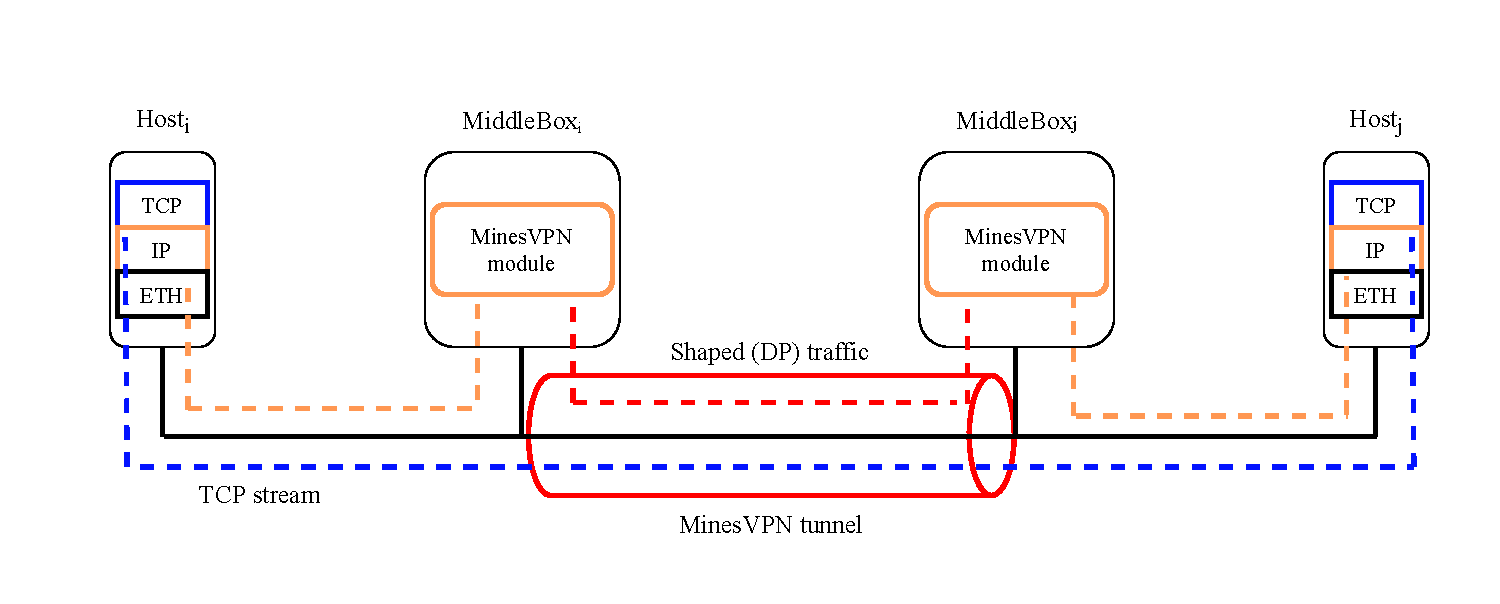
\includegraphics[width=\columnwidth]{figures/Design_highlevel.pdf}
  %  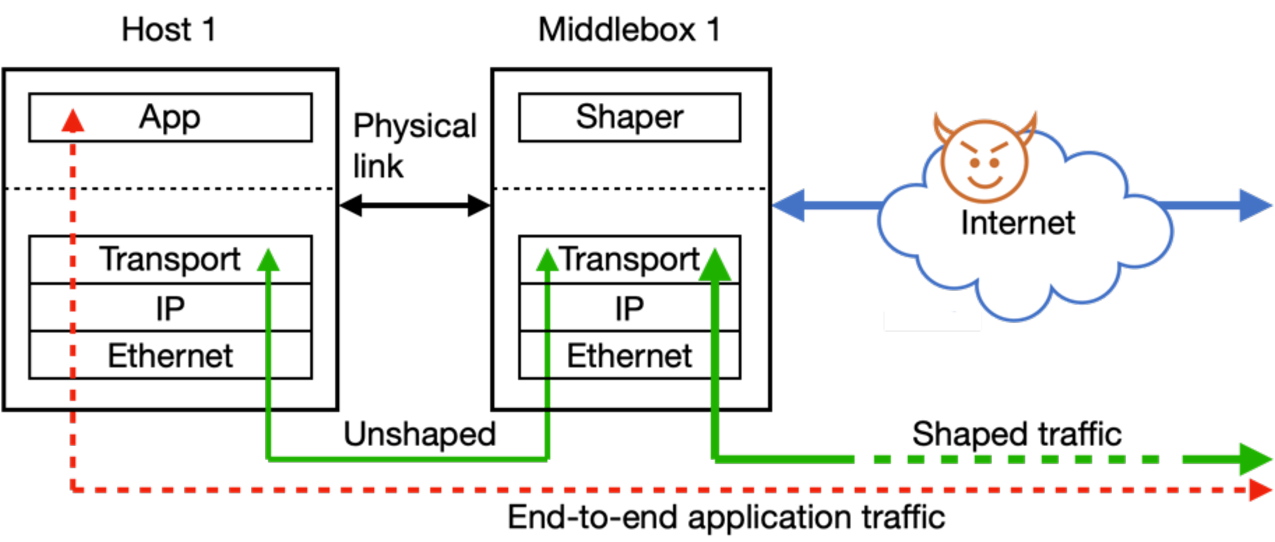
\includegraphics[width=\columnwidth]{figures/minesvpn-overview-half.pdf}
  %  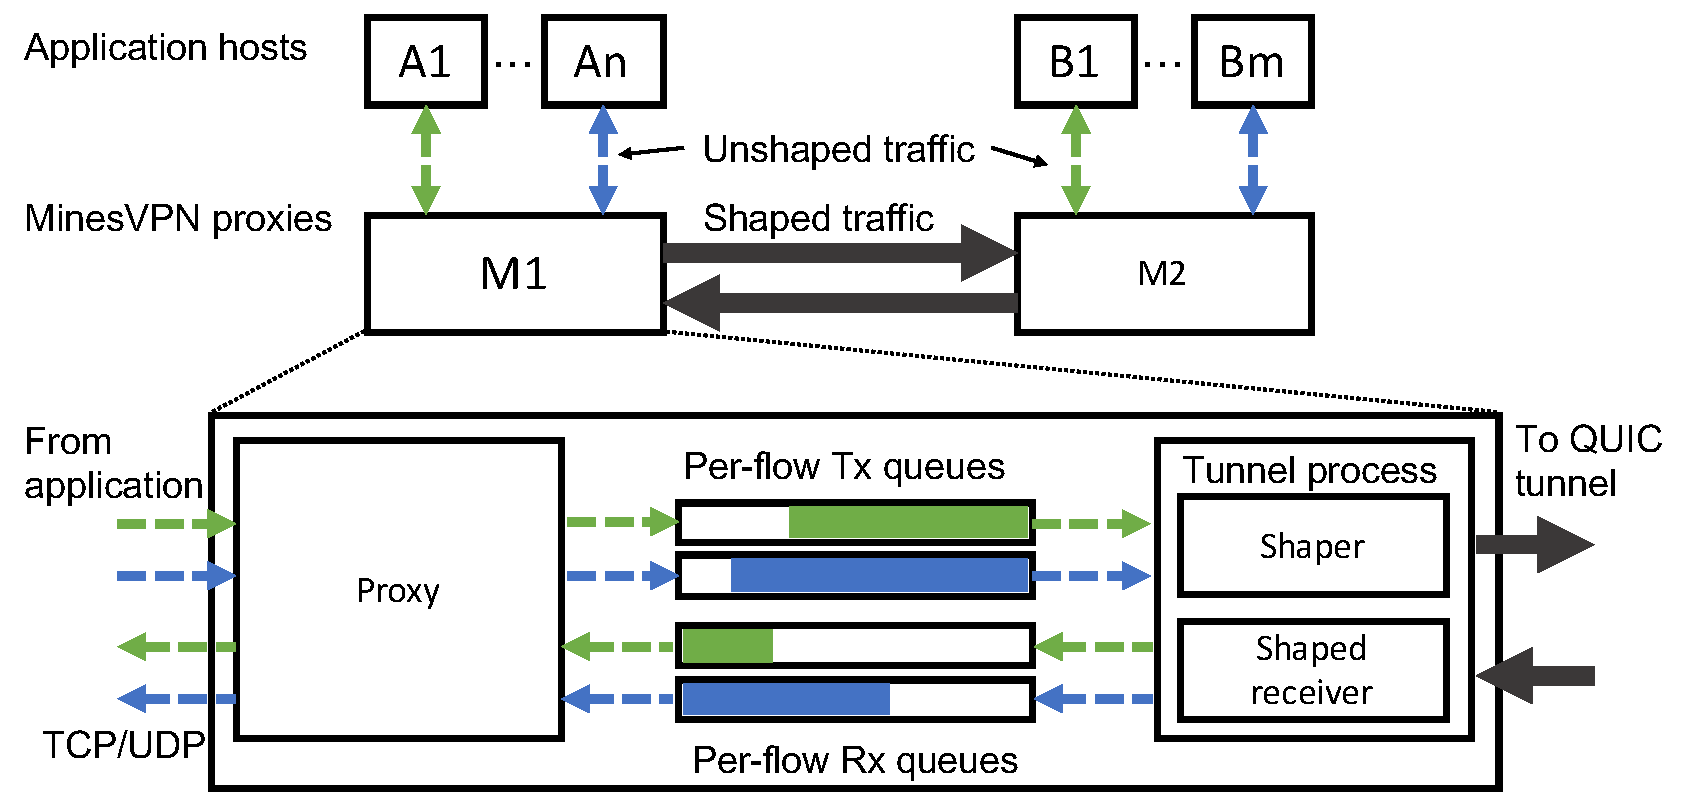
\includegraphics[width=\columnwidth]{figures/minesvpn-arch4.pdf}
  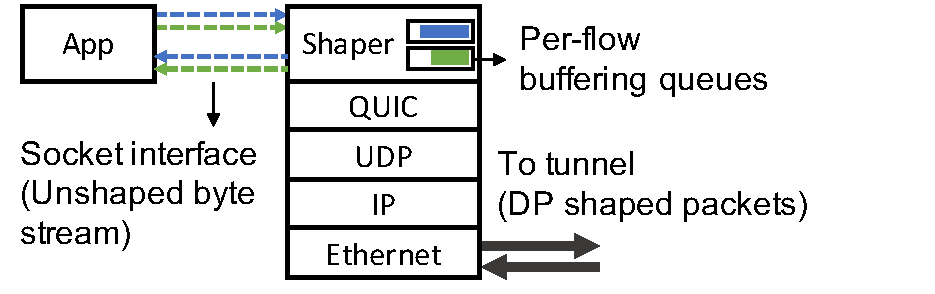
\includegraphics[width=\columnwidth]{figures/design2.pdf}
  \caption{Overview of tunnel design (one endpoint)
      %\am{Update figure}
  }
  \label{fig:minesvpn-overview}
\end{figure}
\Cref{fig:minesvpn-overview} shows the design of one endpoint of {\sys}’s traffic shaping tunnel. A similar endpoint is deployed on the other end of the tunnel.
The shape of the traffic in the tunnel can be configured independently in each direction. The privacy loss in bidirectional streams is the DP composition of the privacy loss in each direction.
A tunnel endpoint consists of a shaping layer (Shaper) on top of QUIC, which in turn runs on top of a standard UDP stack. 
The first requirement should be fulfilled in the implementation of the tunnel, which falls outside the scope of this thesis.
Our design satisfies the second requirement because QUIC deploys encryption for all data transmission, and both data and dummy are sent through a single QUIC connection, ensuring that the receiver identically acknowledges them. 
Finally, QUIC implements congestion control and loss recovery similar to a normal TCP connection, satisfying the third requirement.

It's worth mentioning that aside from QUIC/UDP, {\sys} has the option to utilize a conventional TCP stack as well.
We have specifically chosen QUIC over TCP for the connection between tunnel endpoints because its concept of streams (as discussed in \Cref{sec:background-quic}) allows us to distinguish between dummy and data at the receiver side without the need for additional headers.
The tunnel endpoints establish a bidirectional QUIC connection and generate DP-sized transmit buffers in fixed intervals, which carry payload bytes from one or more application flows.
In the absence of application payload, a tunnel endpoint transmits dummy bytes, which are discarded at the other endpoint.
QUIC encrypts all outbound packets.

{\sys} adopts a transport-layer proxy architecture: each application terminates a connection with the endpoint connected to it.
The application byte stream is sent to the remote application over three piecewise connections: 
(i) between the application and its local tunnel endpoint,
(ii) between the tunnel endpoints, and
(iii) between the remote tunnel endpoint and the remote application.
This ensures only one active congestion control and reliable delivery mechanism in the tunnel and that all bytes are subject to identical mechanisms.
We rely on the transport-layer proxy architecture and discard tunneling TCP through TCP as TCP-in-TCP tunneling causes TCP meltdown~\cite{honda2005tcpovertcp, tcp-meltdown} problem.
In a TCP-in-TCP tunnel, when the network experiences packet loss, the lower-layer TCP initiates packet retransmission to ensure delivery.
However, the upper-layer TCP protocol is unaware of this packet loss and wrongly interprets the increased delay as a sign of a slow network, leading it to decrease the transmission rate.
Consequently, this slower transmission causes the lower-layer TCP protocol to receive acknowledgments too slowly, further mistaking it as packet loss within the network, and thus triggering retransmission.
This repetitive cycle creates a detrimental effect on network performance known as the TCP meltdown problem~\cite{tcp-meltdown}, significantly degrading overall efficiency.
The other option was to use a TCP-in-UDP tunnel. 
This, however, violates the privacy guarantees of {\sys}.
In presence packet loss, the application TCP protocol retransmits data to guarantee data delivery. 
While, the dummy bytes that are injected in the traffic shaping tunnel are not retransmitted, making them observable for adversary. 


\section{Tunnel Design and Operations}\label{sec:tunnel-design}
Now, we describe the fundamental operations that a well-designed {\sys} tunnel must support.
Irrespective of its implementation, a {\sys} tunnel must offer a set of essential functionalities, including tunnel setup and teardown, connection establishment and termination, outbound traffic shaping, and inbound traffic processing. 

\paragraph{Tunnel setup and teardown}
Before applications can communicate with each other, a {\sys} tunnel must be set up between their local tunnel endpoints (as described in \Cref{fig:minesvpn-overview}).
The initiator application can optionally send a configuration message to its local tunnel endpoint with the source and destination IP addresses and ports, and a privacy descriptor.
The privacy descriptor indicates the DP parameters to be used for shaping the tunnel traffic.

Upon receiving a configuration message, the local tunnel endpoint establishes a QUIC connection with the remote tunnel endpoint and configures privacy parameters for each direction.
It also initializes three types of bidirectional~streams in the tunnel: control, dummy, and data streams.
One {\em control stream} is used to transmit messages related to the establishment and termination of a connection between the application endpoints. 
A {\em dummy stream} transmits dummy in QUIC packets in the form of STREAM frames.
We should note that we do not use QUIC's PADDING frames as they do not elicit acknowledgements and hence are distinguishable from STREAM frames \cite{rfc9000}.
The tunnel pre-configures a finite number of data streams, which carry payload bytes from one or more application flows.
When the tunnel is inactive for a period of time, one of the tunnel endpoints initiates a termination sequence and closes all open QUIC streams and the tunnel connection.

\paragraph{Connection establishment and termination}
Once a tunnel is ready, applications can establish and terminate connections with each other, which is mediated by the tunnel.
When the initiator application runs a connection establishment handshake with its local tunnel endpoint, the Shaper maps its flow to a per-flow buffering queue and one of the inactive QUIC data streams in the tunnel, and notifies the remote tunnel endpoint.
The remote tunnel endpoint establishes a connection with the receiver application and maps the receiver application's flow with the data stream.
The connection termination handshake is handled similarly by the tunnel endpoints.
The messages for connection establishment and termination are transmitted over the control stream in the tunnel and shaped according to the tunnel's parameters.

\paragraph{Outbound traffic shaping.}
The Shaper accumulates the outbound bytes of an application flow in a buffering queue before it transmits them in packets whose sizes and timing follow a distribution that guarantees DP.
Within a tunnel, the Shaper transmits bytes from all active flows into a differentially-private packet sequence.
At periodic intervals, called DP measurement intervals, the Shaper performs a DP measurement on the per-flow queues to determine the number of bytes $\qlendp$ to be~transmitted according to the tunnel's DP parameters.
It prepares a {\em shaped buffer} consisting of $\payload$ payload bytes and $\dummy$ dummy bytes, where $\payload$ is the minimum of $\qlendp$ and the application bytes available in the buffering~queues, and $\dummy = \qlendp - \payload$, which may lie between 0 and $\qlendp$.
The Shaper then passes the buffer with the position and length of the padding to QUIC. We simulate the functionality of this component with our traffic shaping simulator in \Cref{sec:eval-simulator}.

QUIC transforms the shaped buffer into one or more STREAM frames based on the
congestion window, the flow window of the receiver endpoint, and the MTU
(maximum transmission unit).
It places the padding bytes into a dummy STREAM frame.
QUIC packages the frames into packets, whose length is at most MTU minus the length of the headers and whose payload is encrypted.
QUIC forwards the packets to the UDP layer, which subsequently transmits the prepared packets as quickly as it can, given the line rate of the NIC.

{\sys} configures the DP measurement interval such that the Shaper can prepare each shaped buffer within an interval.
If the preparation time for a buffer exceeds the interval, the Shaper discards the buffer.
This ensures that the buffering queue length does not grow significantly, which in turn controls the overhead incurred due to DP shaping.
We evaluate the impact of the length of the buffering queue and the DP
measurement interval on privacy guarantees and bandwidth overheads using our simulator in \Cref{ch:evaluation}.

\paragraph{Inbound traffic processing.}
A tunnel endpoint receives shaped packets from the tunnel and applies inverse
processing on each packet.
QUIC receives the packet and
sends an ACK to the sender. Subsequently, it decrypts the packet, discards the
dummy frame, and forwards the payload bytes from the remaining STREAM frames to
the application.

\section{Traffic Shaping Simulator}\label{sec:eval-simulator}
We design and implement a traffic shaping simulator to evaluate the bandwidth overhead and privacy guarantees of {\sys}'s.
The simulator helps users to find parameters of {\sys} shaping mechanism that balance the trade-offs between privacy and overhead according to their requirement.
They can use these parameters in the actual {\sys} system, which we designed in \Cref{sec:tunnel-design} and implemented as part of NetShaper paper \cite{netshaper}.
The simulator specifically simulates the functionality of \emph{Outbound Traffic Shaping} component of a tunnel endpoint to evaluate the privacy and bandwidth overheads of our DP shaping strategy.
The simulator consists of four major components: the Inbound Traffic Processor, responsible for receiving and processing collected traces; the Streaming Application, which emulates the behavior of the application that generated the traffic traces; the Single-Producer Single-Consumer Queue, representing the concept of the buffering queue introduced in \Cref{sec:dp-shaping-definitions} as part of our shaping mechanism; and finally, the Traffic Shaping Module, which implements the core shaping mechanism explained in \Cref{subsec:dp-shaping-mechanism}.


\paragraph{Inbound Traffic Processor}\label{subsubsec:design-sim-inbound}
The simulator takes a PCAP file as the input. 
A PCAP file contains the size and timestamp for every packet that exchanged during a communication session.
To reconstruct the traffic shape from a PCAP file, the simulator discretizes time based on a user defined parameter, \emph{time resolution}.
The \emph{Time resolution} defines the finest level of time granularity upon which the simulator relies.
For instance, if we define \emph{time resolution} as $1ms$, the simulator maps the input trace to a time series, where the $i$\textsuperscript{th} element of time series represent the number of bytes transmitted between the $i$\textsuperscript{th} and the $(i+1)$\textsuperscript{th} millisecond of data transmission (the time series is zero when nothing is sent).
As the data \emph{time resolution} decreases, the simulator more closely replicates the actual shape of the input traffic.
We implement this functionality, as well as preprocessing of the input data, as part of the \texttt{DataProcessor} class in simulator~\cite{netshaper_repo}.



\paragraph{Streaming Application}\label{subsubsec:design-simulator-app}
We develop a simulated application that transmits data based on the time series extracted from PCAP files. 
More precisely, at intervals defined by the \emph{time resolution} of the simulator, the application transmits a quantity of bytes determined by the input time series.
The application continues sending bytes until it either finishes the input traces or it receives a termination signal from the traffic shaping module.
Based on the input trace, simulated application can simulate both server and client side traffic shape.
We implement the simulated application as the \texttt{Application} class in the simulator.

\paragraph{Single-Producer Single-Consumer Queues}\label{subsubsec:design-sim-spsc-queue}
In \Cref{sec:dp-shaping-definitions}, we introduced the \textit{buffering queue} to control the maximum information accessible by an adversary in a predefined time window.
We implement this in the simulator as a simple single-consumer, single-producer queue.
The producer is the streaming application, and
the consumer is our DP traffic shaping module.
The simulated application, as the producer for this queue, pushes a specified number of bytes, based on the input trace, into the queue.
We define a parameter, \emph{shaping interval}, corresponding to the intervals of $T$ seconds we introduced in \Cref{subsec:dp-shaping-mechanism}.
Every $T$ seconds, the shaping module dequeues data with a size determined by
the DP traffic shaping mechanism.



\paragraph{Traffic Shaping Module}
The traffic shaping module is the core part of our simulator where we implement the differentially private traffic shaping mechanism.
Every $T$ seconds, the traffic shaping module determines the number of bytes to be transmitted based on a DP measurement on the size of the application queue, $\qlendp$.
Then, it dequeues $\payload = \min(\qlendp, \qlen)$ from the queue, where $\qlen$ is the number of available bytes in the queue at the measurement time. 
If $\qlendp$ is larger that $\payload$, the traffic shaping module adds $\dummy = \qlendp - \payload$ bytes of dummy data to the transmitted traffic.
We also extend the traffic shaping module to implement constant-rate and Pacer~\cite{mehta2022pacer} traffic shaping to allow comparison between these approaches and {\sys}. 



\chapter{Evaluation}\label{ch:evaluation}
Our evaluation answers the following questions.
(i) How well does {\sys} mitigate state-of-the-art network side-channel attacks?
(ii) What are the overheads associated with varying DP configuration parameters?
(iii) What are {\sys}'s overall costs on privacy and bandwidth for different classes of applications?
(iv) How do {\sys}'s privacy guarantees and performance overheads compare to prior techniques?


For our experiments, we use a AMD Ryzen 7 7700X desktop with eight 4.5 GHz CPUs, 32 GB RAM, 1 TB storage, and a GTX 4090 GPU.
We use two applications as case studies, a video streaming service and a medical web service, which we describe below.
From each application, we collect two different sets of traces to evaluate the privacy and overhead of our shaping mechanism.
\paragraph{Video service.}
The video streaming service is hosted on an Nginx 1.23.4 web server and is used to serve 100 YouTube videos in 720p resolution.
The videos are stored on a standard file system on the host OS and have durations ranging from 5 min to 130.3 min (median 12.6 min) and sizes ranging from 2.7 MB to 1.4 GB (median 73.7 MB).
We stream the first 5 minutes of each video 100 times and collect the traces, leading to 10000 traces in total.

\paragraph{Web service.}
The web service is also hosted on Nginx 1.23.4 and is used to serve a corpus of 100 static HTML pages of a medical website.
The web pages are stored on a standard file system on the host OS and have sizes ranging from 54 KB to 147 KB (median: 90 KB).
Similar to the video dataset, we request each webpage 100 times, resulting in a dataset with 10000 traces in total.
%


In \Cref{sec:eval-tcn}, we provide a brief overview of our TCN-based video identification attack, where we use temporal neural networks (TCN) to map the pattern of the traffic trace to its content.
Then, in \Cref{sec:eval-empirical-privacy} we use our TCN-based video identification attack to evaluate the privacy of DP traffic shaping empirically.
In \Cref{sec:eval-privacy-params}, we measure the effect of various parameters in our system on the privacy loss associated with our DP shaping mechanism. 
In \Cref{sec:eval-bw}, we measure the bandwidth and latency overheads of DP shaping mechanism with two different application: video streaming and web services.
Finally, we compare overheads of {\sys} with other traffic shaping techniques.  


\section{TCN-based Video Identification}\label{sec:eval-tcn}

Beauty and the Burst~\cite{schuster2017beautyburst} uses Convolutional Neural Networks (CNNs) for video identification. 
CNNs have been shown to be effective in sequence modeling for decades~\cite{hinton1990connectionist}.
However, there are two problems with using a convolutional neural network as a sequence modeler.
First, convolutional layers applied to a sequence are not inherently causal, meaning that they look into future samples of a sequence to decide the output for the current sample.
Secondly, convolutional neural networks lack a deep effective history size of past samples in the sequence (i.e. their effective history is bounded to the number of samples that kernel can cover from the past).
To address these problems, Bai\etalc{bai2018empirical} proposed a new architecture called Temporal Convolutional Network (TCN).
The TCN utilizes a one-dimensional fully-convolutional network~\cite{long2015fully} equipped with causal dilated convolutions~\cite{oord2016wavenet}, allowing it to examine deep into the past to produce an output for the sequence at any given moment.
They added a generic residual block from input to output.
The architecture is shown in the \Cref{fig:tcn-arch}.
We evaluate the effectiveness of TCN model for network side-channel attacks in \Cref{sec:eval-empirical-privacy}.



\begin{figure}[t]
  \centering
  %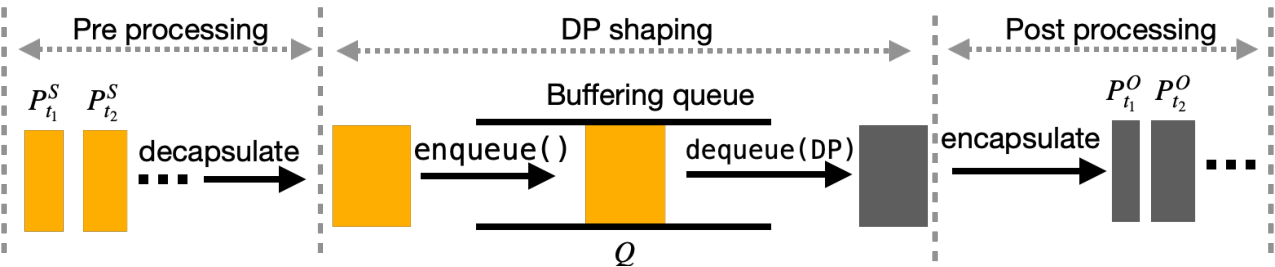
\includegraphics[width=\columnwidth]{figures/DPshaping_concept_vertical.pdf}
  %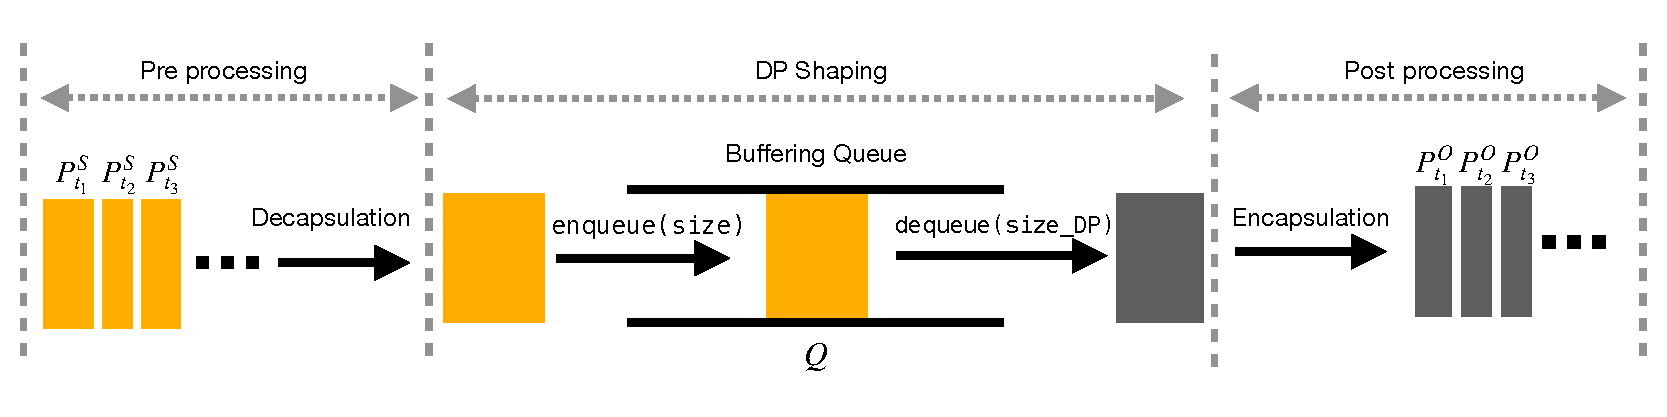
\includegraphics[width=\columnwidth]{figures/DPshaping_concept_horizontal.pdf}
  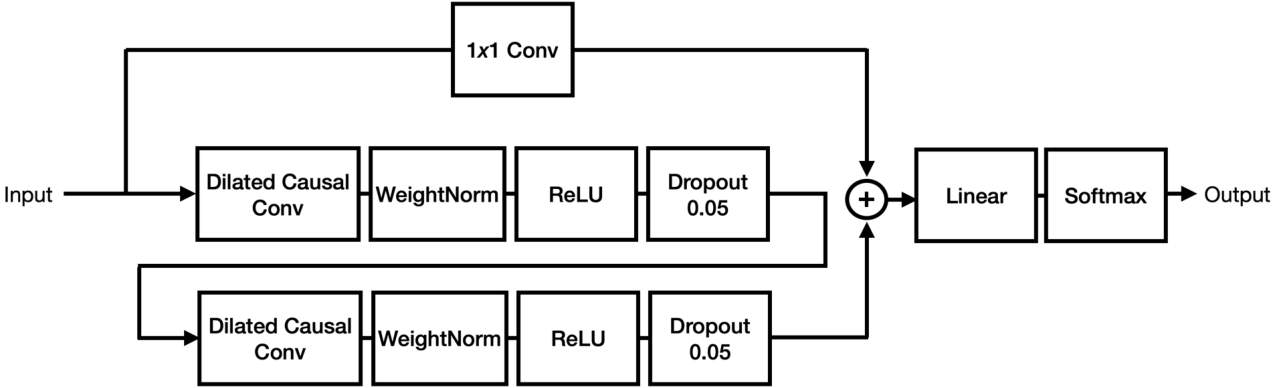
\includegraphics[width=\columnwidth]{figures/TCN_arch.pdf}
  \caption{TCN model architecture.}
  \label{fig:tcn-arch}
\end{figure}



\section{Empirical Privacy Evaluation}\label{sec:eval-empirical-privacy}
We start with an empirical evaluation of the privacy offered by {\sys}'s traffic
shaping.
To evaluate privacy empirically, we first establish the baseline for comparison, which is attacker accuracy, precision, and recall on unmodified (\ie unshaped) traces.
We set up the video service and a video client as two Amazon AWS VMs placed in Oregon and Montreal, respectively.
The client streams the first 5 min of all videos of our video dataset over HTTPS and collects the resulting network packet traces using tcpdump.
We also filter our dataset comprising 10,000 traces and 100 videos to reduce it to a smaller dataset consisting of 40 videos and 4,000 traces.
We evaluate the Beauty and the Burst (BB) model and our TCN-based model with the collected traces using both small and large datasets.
The objective of the models is to determine the corresponding video title for a given trace. 
For each model, we transform each packet trace into a sequence of burst sizes
transmitted within 1s windows.
Therefore, the input to the classifier is a time series representing burst sizes with burst length of 1 second.
We normalize the time series by dividing each burst size by the total size of the corresponding trace.
For each dataset, we use 80\% of traces to train the model and 20\% of traces to test it. 
We train both models for 1000 epochs\footnote{An epoch refers to one complete pass through the entire training dataset during the training.} and report the accuracy, precision, and recall on the test data.
\Cref{tab:attack-performance} represents the result for both models with the two datasets.
Our TCN model outperformes BB model on both datasets. 
Specifically, BB struggles with the larger dataset and its accuracy drops to random guess. 
The presence of residual layers in TCN makes it a better choice for a larger dataset.
\begin{table}[h]
  \centering
  \caption{Attack Performance on unshaped traffic}
  \begin{tabular}{|l|c|c|c|c|}
    \hline
    \textbf{Attack} & \textbf{\# of videos} & \textbf{Accuracy} & \textbf{Precision} & \textbf{Recall} \\ 
    \hline
    \multirow{2}{*}{TCN} & 100 & 0.995 & 0.99 & 0.99 \\ 
                         & 40  & 0.996 & 0.99 & 0.99 \\ 
    \hline
    \multirow{2}{*}{BB}  & 100 & 0.005  & 0.005 & 0.01 \\ 
                         & 40  & 0.61  & 0.49 & 0.63 \\ 
    \hline
  \end{tabular}\label{tab:attack-performance}
\end{table}

Next, we evaluate the efficacy of our differentially-private shaping mechanism against both BB and TCN attacks with the small dataset.
We did not consider the large dataset for this task because the BB model failed to classify the baseline unshaped traffic, making it impossible to see the effectiveness of the DP shaping mechanism for this attack.
The performance of the DP traffic shaping depends on several parameters: the window length $\winlen$, the sensitivity for neighboring streams $\ssens$, the length of the DP measurement interval $\dpintvl$, and the privacy loss $\varepsilon_{\winlen}$.
The privacy of the mechanism, however, is characterized by the privacy loss, $\varepsilon_{\winlen}$
Therefore, we fix values of $\ssens$, $\winlen$, and $\dpintvl$ and measure the accuracy of classifier for varying values of $\varepsilon_{\winlen}$.
As both of attacks fail to perform effectively with small values of $\varepsilon_{\winlen}$ (\ie lower privacy loss), we increment $\varepsilon_{\winlen}$ until one of the attacks yields an accuracy beyond random guessing (\ie $\varepsilon_{\winlen} \in [100, 43000]$).
Our goal is to provide intuition about practical values of $\varepsilon_{\winlen}$ that are sufficient to thwart a side-channel~attack.

We set (i) $\winlen = 5s$ to align with the 5s video segments that comprise the videos, (ii) $\ssens = 1 MB$, which covers 97\% of the video streams in our dataset, and (iii) $\dpintvl = 1s$, which leads to composing the privacy loss over $\varnumupdates = 5$ DP measurements of the buffering queues.

We use 4000 traces of 40 videos, each with 5 minutes duration (\ie small dataset).
For each value of $\varepsilon_{\winlen}$, we transform each unshaped trace into a shaped trace using our simulator to generate a total of 4000 shaped traces.
We train the classifier on 3200 shaped traces and measure the accuracy of the attack model on 800 shaped traces.

\Cref{fig:empirical-privacy} shows the average (markers) and the standard deviation (shaded region) of the accuracy of each classifier over three runs on the shaped traces.
While BB does not perform well for any values of $\varepsilon_{\winlen}$, TCN can be thwarted only for $\varepsilon_{\winlen} < 1000$ with {\sys} (\ns).
The BB and TCN accuracy on unshaped traffic ({\base}) is 0.61 and 0.99, respectively (see \Cref{tab:attack-performance}).
Note that large values of privacy loss (\ie $\varepsilon_{\winlen} \leq 1$) does not provide meaningful theoretical privacy guarantees.
For example, $\varepsilon_{\winlen}=10$ means that given a trace, in the worst-case, the probability that the adversary can correctly identify the video title is $e^{10} \approx 22000$ times larger than the probability that the adversary fails to classify it correctly.
Nonetheless, in practice, we observe that small perturbations with large privacy losses are enough to thwart the state-of-the-art attacks.
This observation highlights the large gap between theoretical guarantees and empirical evaluation of side-channel attacks, which has two important implications: First, the successful mitigation of present attacks by a defense doesn't assure its efficacy against future, more sophisticated attacks.
Second, these findings encourage the development of network side-channel defense mechanisms and their subsequent evaluation based on theoretical privacy considerations, because the empirical evaluation can potentially overestimate the effectiveness of these mechanisms.


\begin{figure}[t]
  \centering
  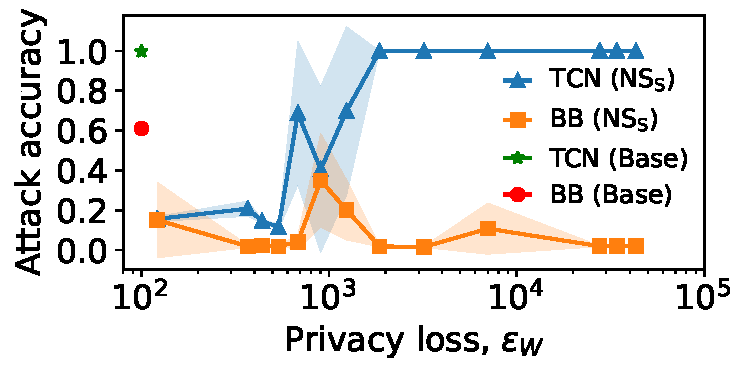
\includegraphics[width=\columnwidth]{plots/accuracy_vs_privacy_loss_video.pdf}
  \caption{Classifier accuracy on shaped traces.
      %    \am{Change label from {\ns} to {\nssim}}
  }
  %\am{How is the blue shaded area going higher than accuracy of 1.0?}\as{The
      %blue shaded area is +-std so it can be larger than one or smaller than
      %zero.}
  \label{fig:empirical-privacy}
\end{figure}

\section{Impact of Privacy Parameters}\label{sec:eval-privacy-params}
We, now,  evaluate how $\varepsilon_{\winlen}$ varies with $\sigma_\dpintvl$, $\varnumupdates$, and $\ssens$.
All analyses use $\delta_\winlen = 10^{-6}$ for two different classes of applications: applications with high sensitivity such as video streaming and applications with lower value of sensitivity such as web browsing.
The sensitivity value represents the highest potential change in the buffering queue size when two distinct traffic traces pass through the shaping mechanism.
If the change in queue size surpasses the sensitivity value, it results in a privacy loss exceeding the intended $\varepsilon_{\winlen}$ threshold.
Nevertheless, the privacy guarantees provided by Differential Privacy (DP) remain applicable even in cases where the privacy loss exceeds the sensitivity, resulting in traffic shaping with larger privacy loss values.


\Cref{subfig:high-sensitivity-epsilon-sigma} and \Cref{subfig:low-sensitivity-epsilon-sigma} show the trade-off between privacy loss ($\varepsilon_{\winlen}$) and noise ($\sigma_\dpintvl$) over four different numbers of DP measurements ($\varnumupdates$) for two different setups.
Intuitively, a larger $\sigma_\dpintvl$ implies higher bandwidth overhead due to DP shaping.
Besides that, applications with higher sensitivity, denoted as $\ssens$, particularly require larger values of $\sigma_\dpintvl$ to provide the same levels of privacy guarantees.
For example, for an application with a sensitivity of $\varepsilon_{\winlen}=1MB$, according to \Cref{subfig:low-sensitivity-epsilon-sigma}, to retain a total privacy loss $\varepsilon_{\winlen} = 1$ with at most 4 DP measurements, we need to add noise with $\sigma_\dpintvl = 6 MB$ for each DP measurement.
Meanwhile, to have the same value of privacy loss with 4 DP measurement in an application with a lower sensitivity $\varepsilon_{\winlen}$, we need to add noise with $\sigma_\dpintvl = 0.8 MB$.

The large gap between theoretical privacy guarantees and the effectiveness of the state-of-the-art attacks is also worth highlighting in this context.
For example, $\varepsilon_{\winlen} = 100$ with 4 DP measurements (the approximate configuration that defeats the classifiers in \Cref{fig:empirical-privacy}) only requires $\sigma_\dpintvl < 0.1 MB$ even for high-sensitivity applications.
However, we configure our system to provide theoretical guarantees (\ie small values of privacy loss), and discuss how to amortize bandwidth overheads using concurrent flows without increasing privacy loss in \Cref{sec:eval-bw}.

Using these plots, an application can choose suitable values of $\ssens$ and $\winlen$ to determine the trade-off between $\varepsilon_{\winlen}$ and $\delta_{\winlen}$.
For our web application serving static HTML, we recommend $\winlen = 1s$, since web page downloads in our AWS setup finished within 1s, and $\ssens = 150 KB$, which covers 95\% of the web pages in our dataset.
Similarly, In \Cref{fig:empirical-privacy}, we explain the choices for our video application.
Using $\varepsilon_{\winlen}$ and $\dpintvl$, we can further determine the aggregate privacy loss over longer traffic streams using R\'enyi-DP composition.
For instance, with $\varepsilon_{\winlen} = 1$, $\winlen = 5s$, and $\dpintvl = 1s$, the total privacy loss for a 5 min video, which generates 300 DP measurements at 1s intervals, is 8.92; the total loss for a 1 hr video is 38.8.
We emphasize that {\em $\ssens$ and $\varepsilon_\winlen$ should be selected using trade-off plots similar to \Cref{fig:privacy-microbenchmarks-low-sensitivity} and \Cref{fig:privacy-microbenchmarks-high-sensitivity} independently of the application's dataset.}
Another approach to parameter configuration within our setup involves utilizing a publicly available dataset for the same application, such as a publicly accessible video streaming dataset or web service dataset.
This allows for the independent configuration of parameters, which can then be deployed within our system, irrespective of users' traffic.




\begin{figure}[t]
  \centering
  \begin{subfigure}{0.49\columnwidth}
      \centering
      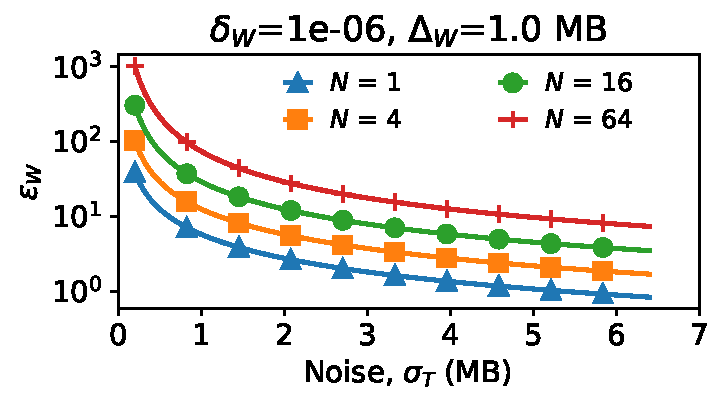
\includegraphics[width=\textwidth]{plots/privacy_loss_VS_noise_std_video.pdf}
      \caption{}
      %        \caption{Noise vs privacy loss}
      \label{subfig:high-sensitivity-epsilon-sigma}
  \end{subfigure}
  \hfill
%    \begin{subfigure}{0.33\textwidth}
  %        \centering
  %
  %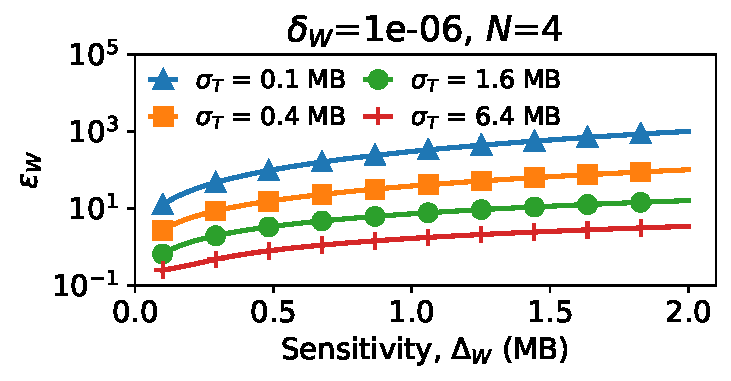
\includegraphics[width=\textwidth]{plots/privacy_loss_VS_sensitivity_video.pdf}
  %        \caption{Sensitivity vs privacy loss}
  %        \label{subfig:high-sensitivity-epsilon-sensitivity}
  %    \end{subfigure}
%    \hfill
  \begin{subfigure}{0.49\columnwidth}
      \centering
      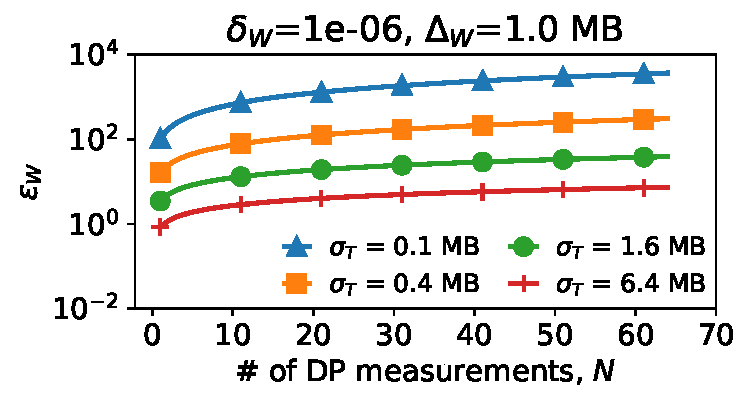
\includegraphics[width=\textwidth]{plots/privacy_loss_VS_query_num_video.pdf}
      \caption{}
%        \caption{\# of DP measurements vs privacy loss}
      \label{subfig:high-sensitivity-epsilon-queries}
  \end{subfigure}
  \caption{
    Per-window privacy loss ($\varepsilon_{\winlen}$) as a function of
    (a) noise ($\sigma_\dpintvl$), and (b) number of DP measurements ($N$).
%    \am{Make notations consistent.}
  }
  \label{fig:privacy-microbenchmarks-high-sensitivity}
\end{figure}


\begin{figure}[t]
  \centering
  \begin{subfigure}{0.49\columnwidth}
      \centering
      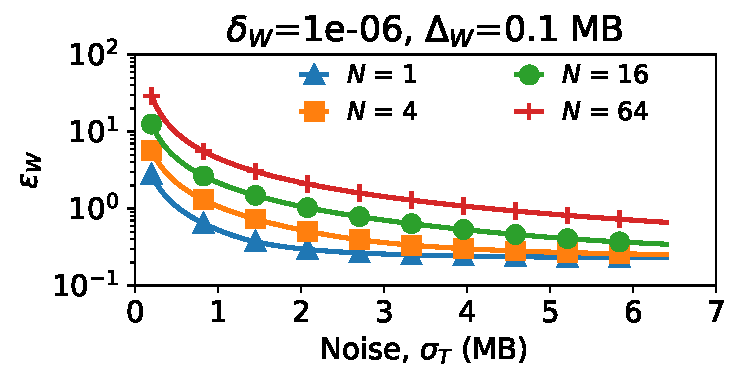
\includegraphics[width=\textwidth]{plots/privacy_loss_VS_noise_std_low_sensitivity.pdf}
      \caption{}
      %        \caption{Noise vs privacy loss}
      \label{subfig:low-sensitivity-epsilon-sigma}
  \end{subfigure}
  \hfill
%    \begin{subfigure}{0.33\textwidth}
  %        \centering
  %
  %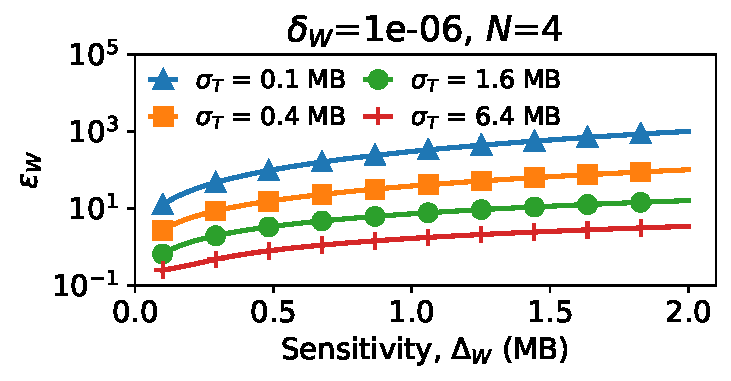
\includegraphics[width=\textwidth]{plots/privacy_loss_VS_sensitivity_video.pdf}
  %        \caption{Sensitivity vs privacy loss}
  %        \label{subfig:high-sensitivity-epsilon-sensitivity}
  %    \end{subfigure}
%    \hfill
  \begin{subfigure}{0.49\columnwidth}
      \centering
      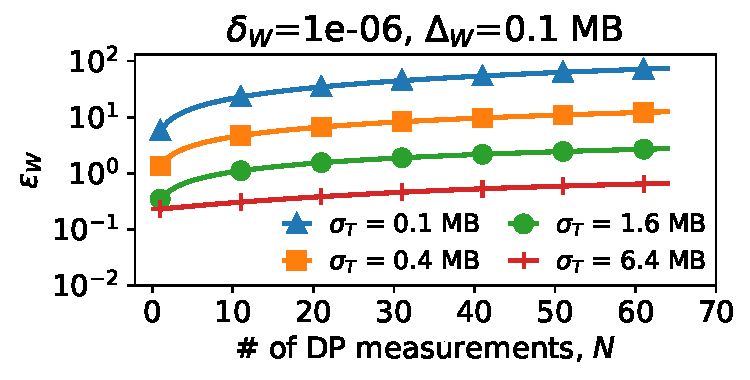
\includegraphics[width=\textwidth]{plots/privacy_loss_VS_query_num_low_sensitivity.pdf}
      \caption{}
%        \caption{\# of DP measurements vs privacy loss}
      \label{subfig:low-sensitivity-epsilon-queries}
  \end{subfigure}
  \caption{
    Per-window privacy loss ($\varepsilon_{\winlen}$) as a function of
    (a) noise ($\sigma_\dpintvl$), and (b) number of DP measurements ($N$).
%    \am{Make notations consistent.}
  }
  \label{fig:privacy-microbenchmarks-low-sensitivity}
\end{figure}

\section{DP Shaping Bandwidth and Latency Overhead}\label{sec:eval-bw}
In this section, we measure the bandwidth overheads of {\sys} for two different applications using our traffic shaping simulator (see \Cref{sec:eval-simulator}).
We present two case studies. 
First, we examine a video streaming service, which serves as a representative example of applications characterized by high sensitivity values due to the substantial fluctuations in traffic rates typically observed in video applications.
Second, a typical web service, representing applications with smaller value for sensitivity.
In both applications, a client initiates a bidirectional communication with the server to retrieve content.
We apply traffic shaping in both directions, customizing the parameters to match the traffic characteristics specific to each direction of communication.


\subsection{Case Study: Video Streaming}\label{subsec:eval-bw-video}
In this section, we examine the effect of different privacy settings on bandwidth overhead for video streaming clients.

We run experiments with three values of the DP measurement interval $\dpintvl$ for the server:
100ms, 500ms, and 1s, and we use $\ssens = 1 MB$ and $\varepsilon_{\winlen} = 1$.
For all experiments, we set the DP parameters for client request traffic as follows: $\ssens = 200$~bytes, $\winlen = 1s$, $\dpintvl = 100ms$, and $\varepsilon_{\winlen} = 1$.
For the server responses, we configure DP parameters as follows: $\ssens = 1 MB$~bytes, $\winlen = 5s$, $\dpintvl = 1 s$, and $\varepsilon_{\winlen} = 1$.
We use different set of parameters for communication from server to client and vice versa due to the different characteristics of traffic in each direction.
Periodically, at intervals of 5 seconds, client sends a small web request  to the server to download next segment of the video. 
In the reverse direction, server transmits segments to the client one by one.
Compared to the small client's request, segments are larger and have bursty traffic pattern.
As the client requests each segment preemptively, as long as the server delivers next segment within the 5 seconds, the client can play video seamlessly. 
We run experiments with 1, 16, and 128 video clients; each client requests one video randomly selected from the dataset.
For each set of configurations, we measure the per-flow relative bandwidth overhead for the video streams in the simulator.


\begin{figure}[t]
  \centering
  \begin{subfigure}{0.49\columnwidth}
      \centering
      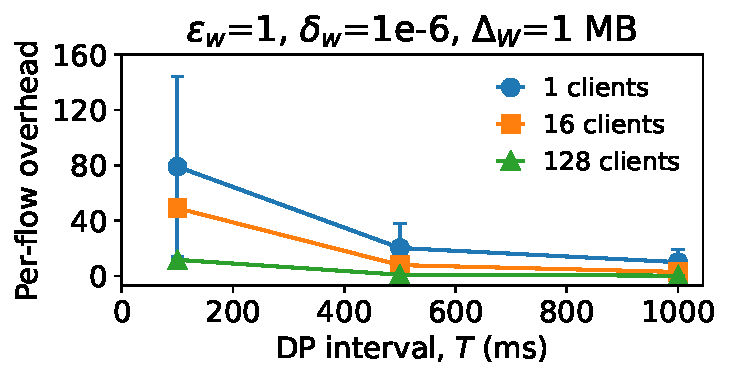
\includegraphics[width=\textwidth]{plots/overhead_vs_dp_interval_video.pdf}
      \caption{BW overhead vs DP interval (video)}
      \label{fig:video-overhead-vs-dpInt}
  \end{subfigure}
  \hfill
  \begin{subfigure}{0.49\columnwidth}
      \centering
      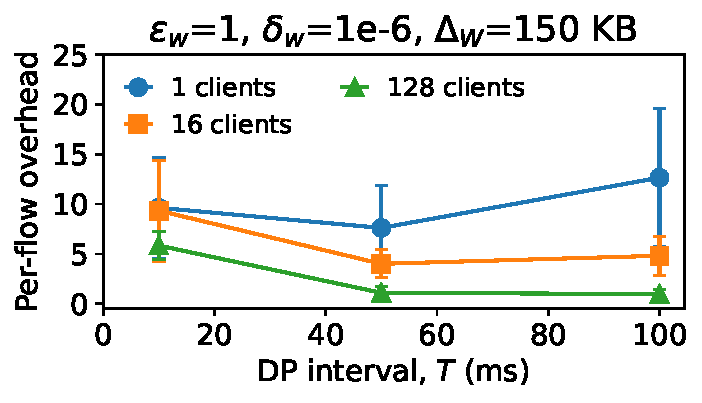
\includegraphics[width=\textwidth]{plots/overhead_vs_dp_interval_web.pdf}
      \caption{BW overhead vs DP interval (Web)}
      \label{fig:web-overhead-vs-dpInt}
  \end{subfigure}
  \caption{Video Streaming and Web Service; Bandwidth overhead for different values of DP interval.
  }
\end{figure}


\begin{figure}[t]
  \centering
  \begin{subfigure}{0.49\columnwidth}
      \centering
      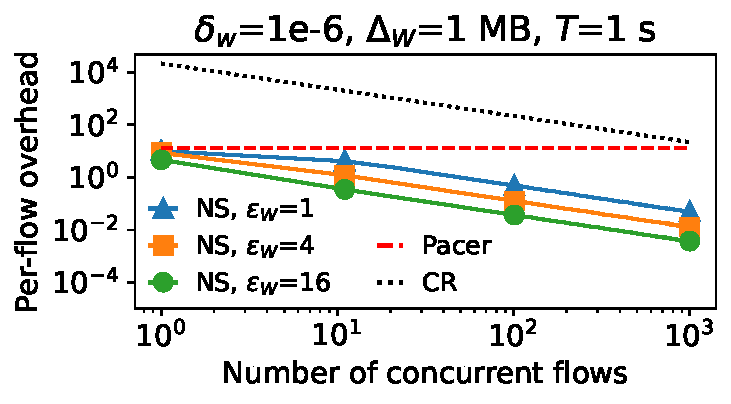
\includegraphics[width=\textwidth]{plots/overhead_vs_number_of_traces_video_loglog.pdf}
      \caption{Video streaming.}
      \label{fig:video-overheads-compare}
  \end{subfigure}
  \hfill
  \begin{subfigure}{0.49\columnwidth}
      \centering
      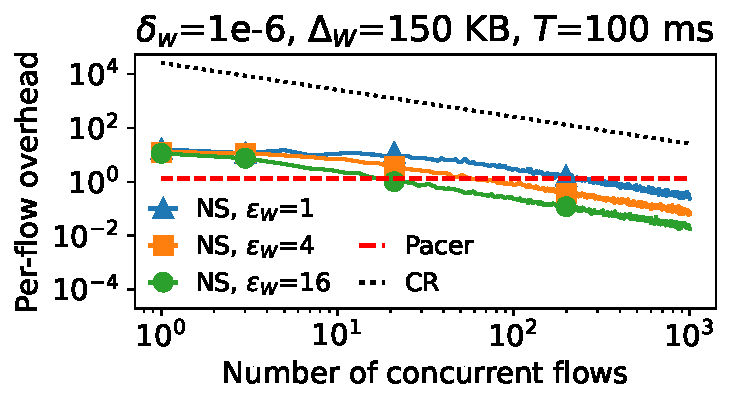
\includegraphics[width=\textwidth]{plots/overhead_vs_number_of_traces_web_loglog.pdf}
      \caption{Web service.}
      \label{fig:web-overheads-compare}
  \end{subfigure}
  \caption{Relative bandwidth overheads of {\sys} ({\ns}), constant
      shaping ({\constshape}), and Pacer.
  }
\end{figure}


\paragraph{Bandwidth overhead.}
\Cref{fig:video-overhead-vs-dpInt} shows the average per-flow relative bandwidth overhead as a function of different intervals and for varying number of clients.
The relative bandwidth overhead of a video is the number of dummy bytes transmitted normalized to the size of the unshaped video stream.
The error bars show the standard deviation in latency and bandwidth overhead.
We observe that the relative overhead decreases with larger values of $\dpintvl$.
While our simulation does not allow for the direct measurement of end-to-end latency, it's important to note that larger values for $\dpintvl$ result in data transmission occurring at more extended intervals, which can contribute to increased latency.
Therefore, the results show the trade-off between latency and bandwidth. 
A larger DP measurement interval implies higher download latency but fewer measurements and lower noise added to the payload, thus yielding a lower bandwidth overhead.
Thirdly, with multiple concurrent streaming clients, the bandwidth overhead is amortized.
Overall, {\sys}'s shaping can secure video streams with low bandwidth overheads.


\paragraph{Comparison with other techniques.}
\Cref{fig:video-overheads-compare} shows the per-flow relative bandwidth overhead of {\sys} ({\ns}) for video streaming application for varying with number of concurrent flows and for different values of $\varepsilon_{\winlen}$.
Except $\varepsilon_{\winlen}$, we use the same of parameters that we proposed in the beginning of this section.
We also compare with the overheads~that would be incurred due to constant rate
shaping ({\constshape}) and~Pacer \cite{mehta2022pacer} (see \Cref{subsubsec:background-defenses-pacer}), a SOTA system
that traffic shaping on a per-client request basis.

For {\constshape}, we configure the peak load for video service corresponding to
transmitting 1.7MB in every 5s, which is corresponding to transmitting the largest segment size in our video dataset. In other words, the {\constshape} mechanism always sends data at the maximum rate required to send a segment in our dataset.
In Pacer, for video service, we pad a segment at $i$\textsuperscript{th} index
in a video stream to the largest segment size at that index across all videos in the dataset. 
Even with the lowest privacy loss, $\varepsilon_{winlen}=1$, {\ns} add the same level of overhead as Pacer and 3 orders of magnitude less overhead than {\constshape}.  
Besides that, {\ns} can further amortize its overheads
among multiple concurrent streams within the tunnel without compromising privacy.





\subsection{Case Study: Web Service}\label{subsec:eval-bw-web}
In this section, we examine the effect of different privacy settings on bandwidth overhead for a web service.
We   
As we mentioned, we expect the values of DP measurement interval affects the communication end-to-end latency.
We choose smaller values for $\dpintvl$ for web service as compared to video streaming applications as web applications are delay-sensitive.
For the server responses, we use three values for DP measurement intervals, $\dpintvl$: 10 ms, 50 ms, 100 ms, and configure other parameters as follows: $\ssens = 150 KB$, $\winlen = 1s$, and
$\varepsilon_{\winlen} = 1$.
For the client requests, we use $\ssens = 200 B$, $winlen = 1s$, and $\varepsilon_{\winlen} = 1$.
We run experiments with 1, 16, and 128 video clients; each client requests a random webpage from the dataset.



\paragraph{Bandwidth overhead.}
\Cref{fig:web-overhead-vs-dpInt} shows the average per-web page relative bandwidth overhead, across all web page requests.
The bandwidth overhead for web traffic first reduces with increasing DP measurement interval from 10ms to 50ms, but interestingly, it increases again
with an interval of 100ms.
This is because, for small web pages, the DP interval of 100ms is larger than the total time required to download web pages.
As a result, additional overhead is incurred due to the padding of traffic in the 100ms intervals.
Similar to video streaming applications, when there are multiple concurrent requests from clients, the relative bandwidth overhead tends to decrease.

\paragraph{Comparison with other techniques.}
\Cref{fig:web-overheads-compare} shows the per-flow relative bandwidth overhead of {\sys} ({\ns}) for a web service for varying with number of concurrent flows and for different values of $\varepsilon_{\winlen}$.
We maintain the remaining parameters at the same values as previously mentioned.
Similar to video streaming, for web service, we compare {\sys} ({\ns}) with Pacer and constant rate shaping ({\constshape}).
For {\constshape}, we configure the peak load for web service corresponding to
transmitting 57KB in every 50ms, which is corresponding to transmitting the largest web page in our dataset.
For web services, Pacer pads all web pages to the largest page size, which is 147KB in our dataset.
Similar to video streaming case study, {\ns} introduces overheads that are several orders of magnitude smaller when compared to {\constshape}.
However,{\ns} requires more than 20 flows to achieve lower overhead than Pacer.
Pacer shapes server traffic only upon receiving a client request and does not
shape client traffic. 
Thus, it leaks the timing and shape of client requests, which could potentially reveal information about the server responses \cite{chen2010reality}.
{\sys} shapes traffic in both directions, which incurs higher overhead at the cost of stronger privacy than Pacer. 
\chapter{Conclusion}\label{ch:conclusion}
{\sys} is a novel mitigation for side-channel attacks. 
It relies on the strong notion of differential privacy to provide theoretical privacy guarantees, while introducing minimal overheads. 
{\sys} is extensively configurable, allowing users to change the privacy-utility trade-offs based on their requirements across different range of applications. 
We are confident that {\sys} has the potential to put an end to the arms race in network side-channel attacks and defenses.  
Furthermore, we have designed {\sys} in a modular fashion, ensuring that it can be deployed seamlessly at any point along the traffic path without requiring any modifications to the application itself. 

We conclude the thesis by providing an overview of {\sys}'s limitations and elaborating on potential future directions for this project.

\section{{\sys} Limitations}\label{sec:conclusion-limitations}
\paragraph{Client-Server Communication Model.}
A specific limitation of {\sys} is its communication model, which assumes all communication between the client and server passes through a single differentially-private traffic shaping tunnel.
In situations where a single client communicates with multiple servers via different tunnels, the correlation between these communications has the potential to result in additional information leakage.
Current communication model inherently fails to capture the privacy loss of such scenarios, leading to lower-than-expected privacy guarantees.

\paragraph{Lack of Anonymization.}
{\sys} does not provide complete anonymity.
Specifically, it does not capture the privacy loss due temporal correlation across multiple tunnels.
When a client sends a message to a server that traverses multiple independent instances of the {\sys} tunnel, the temporal correlation between the traffic shaping in these tunnels can inadvertently leak information. 
Using this information, the adversary can reveal the communication parties.

\paragraph{Middlebox and Trusted Computing Base.}
{\sys} assumes the traffic shaping middlebox to be trusted and bug-free.
Nonetheless, it's essential to acknowledge that the middlebox itself may be susceptible to various types of attacks and implementation flaws. Incorporating the middlebox hardware and software stack into the trusted computing base without conducting a rigorous assessment of its correctness and security could introduce vulnerabilities.

\section{Future Research Directions}\label{sec:conclusion-future}
\paragraph{Multi-Party Correlated Communication.}
As a future research direction, DP guarantees of {\sys} can be extended to multi-party communication, when the communication between parties are not necessarily independent.
In many internet applications,  simultaneous communications with distinct entities are interdependent.
For example, many businesses use online advertising platforms such as Google Ads to create and run ads on various websites.
Therefore, every time a user requests the website, the web browser retrieves content from both the web server hosting the website and the online advertising platform that hosts the website's Ads.   
This is, in fact, an example of a one-to-many correlated communication setup.
In standard definition of differential privacy, we assume data points to be independent.  
However, measuring the privacy loss when entries of database are correlated is challenging. 
This is an interesting future path for research.

\paragraph{{\sys} and Programmable Networks.}
We propose a design for {\sys} based on proxy model, where it receives traffic, decapsulates it, performs DP shaping, encapsulates data, and sends it over the tunnel.
Implementing this functionality at the application layer results in increased end-to-end communication latency, as each packet must traverse the kernel network four times before arriving at the destination.
Recent advances in programmable networking devices such as programmable NICs and programmable switches~\cite{meier2022ditto} provides an opportunity to offload DP shaping mechanism to the network hardware, which can potentially reduce the latency of {\sys}.

\paragraph{optimized DP Shapnig.}
Current DP shaping mechanism, measures the queue size every $\dpintvl$ seconds.
We know that based on the composition theorem privacy loss increase with every measurement of the queue size. 
However, if the queue size does not significantly change between intervals, DP shaping mechanism can use the measurement of the previous interval without further increasing the privacy loss. 
This is the foundation of new, more sophisticated DP mechanism, known as Sparse Vector Technique for Differential Privacy~\cite{lyu2016understanding}. 
Adapting this form of DP mechanism for our DP shaping is an exciting direction for future research.

%\include{relatedwork}
%\include{model}
%\include{impl}
%\include{discussion}
%\include{conclusions}

%    3. Notes
%    4. Footnotes

%    5. Bibliography
\begin{singlespace}
\raggedright
\bibliographystyle{abbrvnat}
\bibliography{biblio}
\end{singlespace}

% \appendix
%    6. Appendices (including copies of all required UBC Research
%       Ethics Board's Certificates of Approval)
%\include{reb-coa}	% pdfpages is useful here
% \chapter{Differentially Private Multi-Party Communication}
In \Cref{ch:dp-shaping}, we explained our differentially private traffic shaping mechanism. 
In this setup, each end-point only communicates with one other end-point at a time. 
Hence, we excluded e-anonymization attacks, which involve adversaries attempting to uncover the fact that two parties are engaged in communication, rather than revealing the content of the communication.
Furthermore, we assumed a one-hop communication in which the adversary monitors the traffic between two middleboxes.
In order to generalize our findings to scenarios involving multi-party communication, we establish two fundamental communication scenarios: 1- One-to-many communication, and 2- Multi-hop communication. 
We illustrate how we can extend DP guarantees to cover these two scenarios.
Subsequently, we demonstrate that these two communication scenarios adequately serve as building blocks for constructing any arbitrary communication pattern.

\section{One-to-Many Differentially Private Communication}
We assume an application is communicating with $N$ parties at a time.
We extend the notation proposed in \Cref{sec:dp-shaping-definitions} and represent an application stream as a series of $N$ packet sequences:
\begin{equation}
  \istream = <\istream^1, \istream^2, \dots, \istream^N>
\end{equation}
\noindent
where we have:
\begin{align*}
  \istream^1 &= \{{P^{S^1}_1}, {P^{S^1}_2}, {P^{S^1}_3}, \dots \} \\
  \istream^2 &= \{{P^{S^2}_1}, {P^{S^2}_2}, {P^{S^2}_3}, \dots \} \\
  \vdots& \\
  \istream^N &= \{{P^{S^N}_1}, {P^{S^N}_2}, {P^{S^N}_3}, \dots \} 
\end{align*}
\noindent
where $P^{S^k}_i = (l_i^{S^k}, t_i^{S^k})$ indicates that the $i$\textsuperscript{th} input packet sent to $k$\textsuperscript{th} receiving party in communication has length $l_i$ and transmitted at time $t_i$.
\\
\noindent
We make the assumption that all receiving parties are situated behind distinct middleboxes, thereby leading to $N$ parallel communications. \Cref{fig:one-to-many-communication} visually represents this scenario.
This assumption does not restrict the expendability of this scenario as if more than one receiving parties are placed behind the same middlebox, we can merge their packet sequences into one sequence and reduce the number of parallel communications to $N' < N$.   
\begin{figure}[t]
  \centering
  %  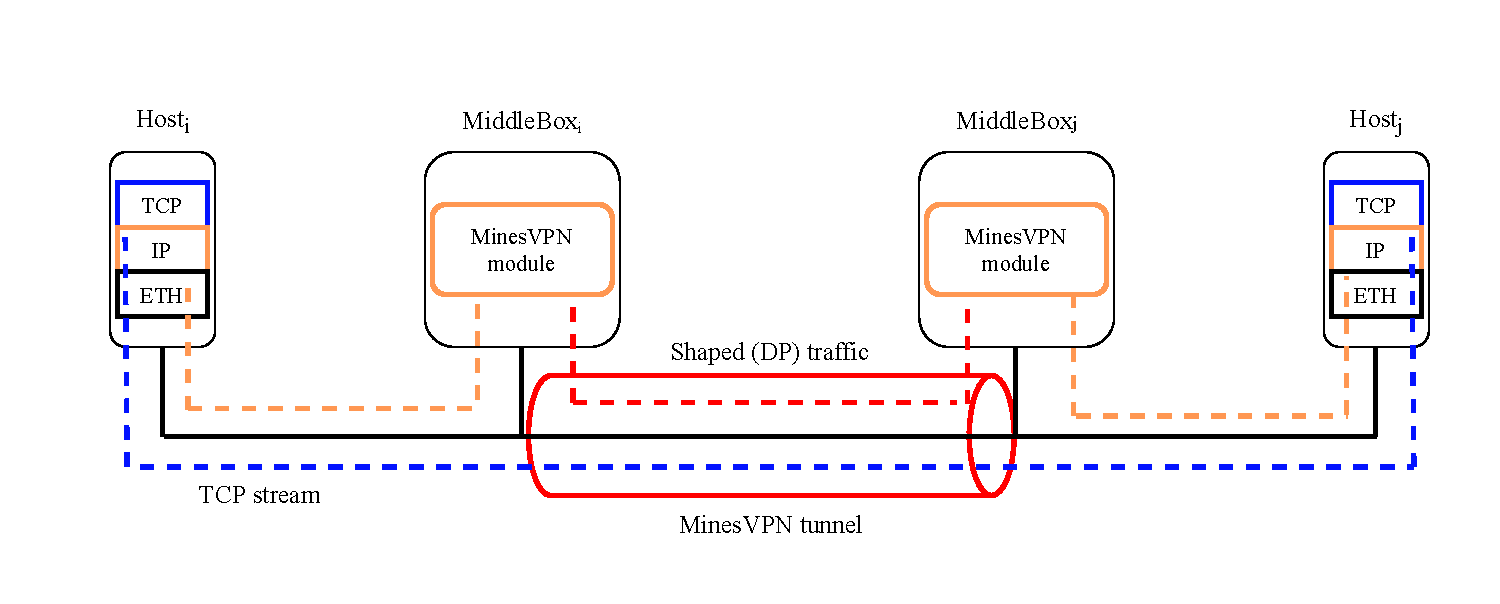
\includegraphics[width=\columnwidth]{figures/Design_highlevel.pdf}
  %  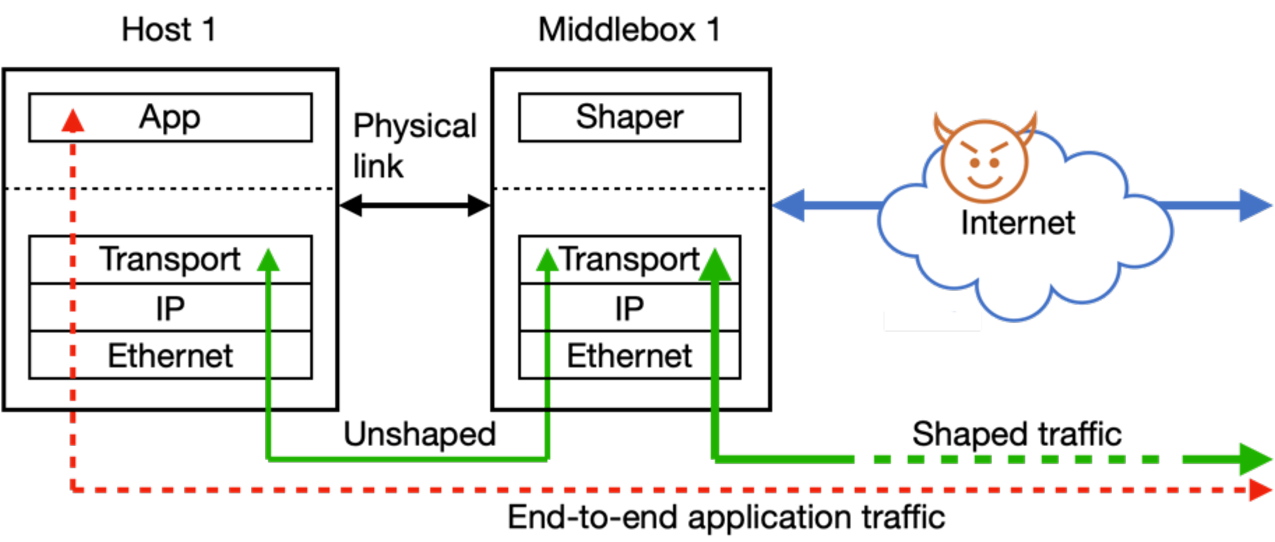
\includegraphics[width=\columnwidth]{figures/minesvpn-overview-half.pdf}
  %  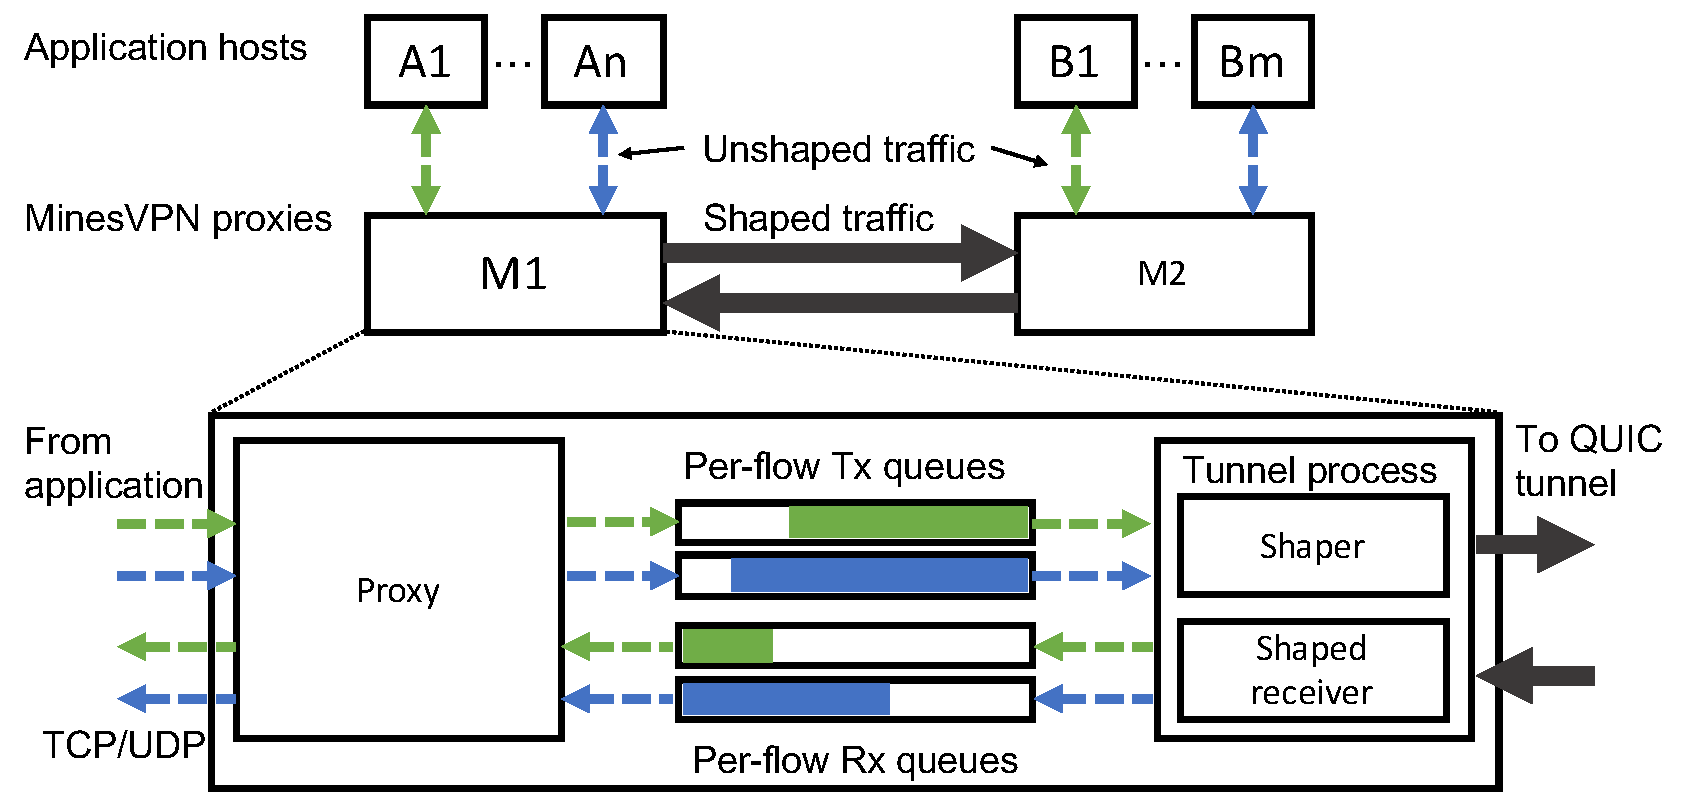
\includegraphics[width=\columnwidth]{figures/minesvpn-arch4.pdf}
  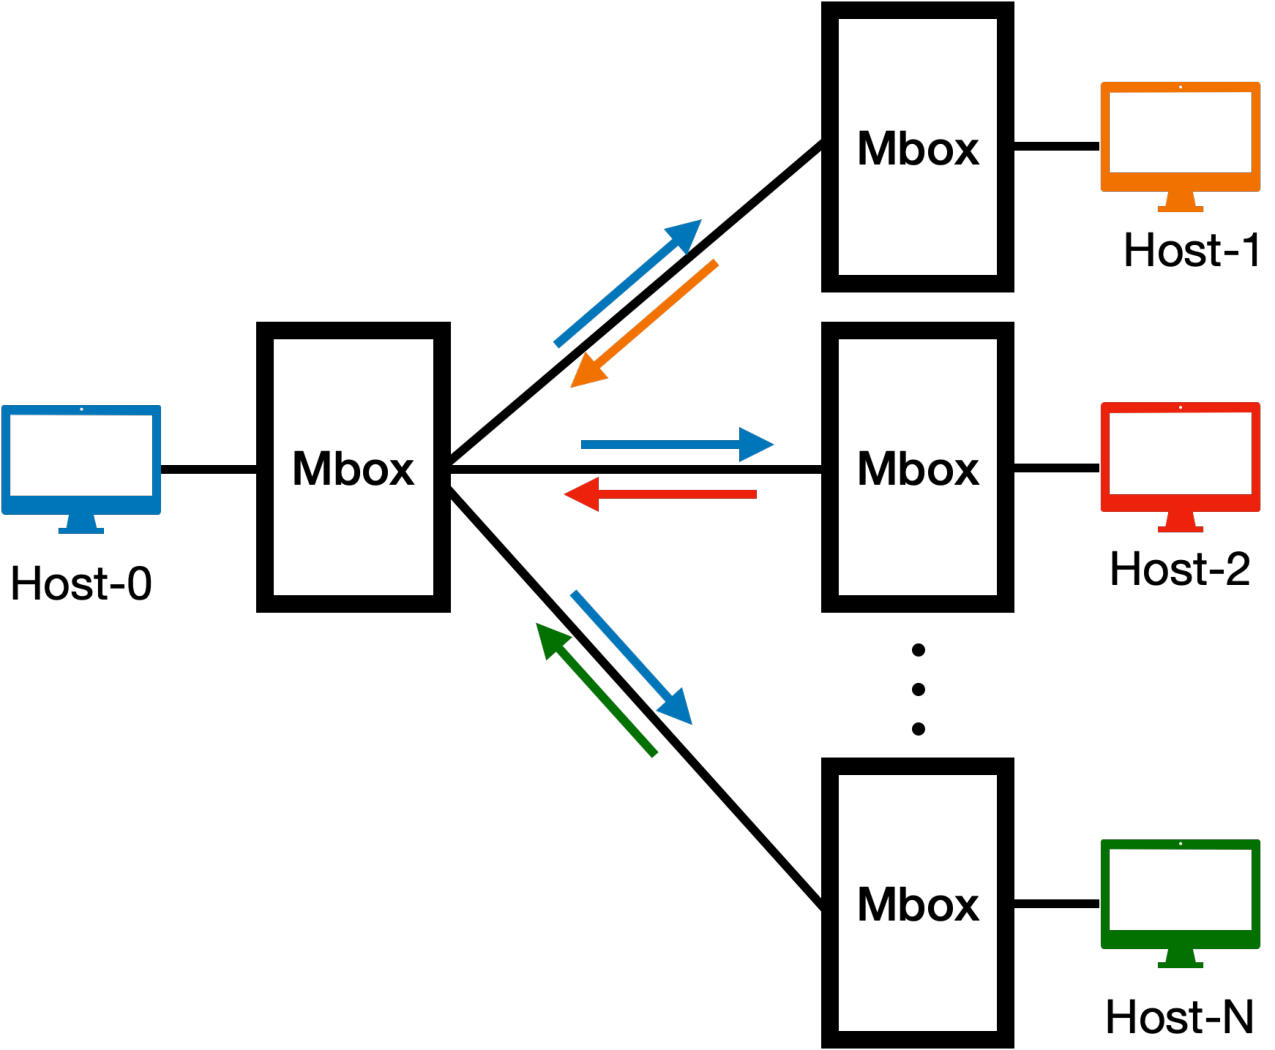
\includegraphics[width=0.7\columnwidth]{figures/one-to-many-communication.pdf}
  \caption{
    One-to-Many parallel communication.
  }
  \label{fig:one-to-many-communication}
\end{figure}



We extend the concept of \textit{buffering queue} that we introduce in \Cref{sec:dp-shaping-definitions} to a \textit{set of $N$ buffering queues} for an application, one for each of pair of communicating parties.  
Each of these queues enqueue the incoming data from application parallel streams with one party within windows of the size of $W$. 
In other words, \Cref{assumption:window} holds true for all $N$ queues simultaneously. 
Similar to \Cref{sec:dp-shaping-definitions}, we define a set of stream subsequences over a window $j$ and represent it with $\istream_j = <\istream^1_j, \istream^2_j, \dots, \istream^N_j>$, such that $k \in [N]:~\istream_j^k = \{P^{\istream^k}_i | P^{\istream^k}_i \in \istream^k~and~t_i^{S^k} \in j\}$. 
Intuitively, a set of stream subsequences is a slice with a length $W$ across all parallel communications with $N$ parties.
We re-define the \Cref{def:neighboring-streams} to match the new setup.
\begin{definition}[Neighboring Series of Streams]\label{def:neighboring-series-stream}
  Two sets of $N$ stream subsequences $S_{j}$ and $\hat{S}_{j}$ transmitted in a window $j$ are neighbors if the L1-norm distance between all corresponding subsequences is at most~$\ssens$ bytes in a window of up to length $\winlen$.
  \\
  In other words: 
  \begin{equation*}
    \forall k \in [n]: {\norm{~S_{j}^k - \hat{S}_{j}^k~}}_1 \leq \ssens
  \end{equation*}
\end{definition}
\noindent
For each subsequence, we define the sensitivity value of its dedicated queue over the intervals of length $T$. 
We represent the sensitivity of a subsequence $S_{j}^k$ with $\qsens^k$: 
\begin{equation}
  \qsens^k = \max_{l = 0}^{\numupdates}~\max_{\streamw{j}^k,
      \hat{\streamw{j}^k}} | \qlent{l}^k - \hat{\qlent{l}^k} |
  \label{eqn:ssens-multi-stream}
\end{equation}
where $\qlent{l}^k$ and  $\hat{\qlent{l}^k}$ are queue lengths of the subsequence $S_{j}^k$ and subsequence $\hat{S_{j}^k}$ at the beginning of the $l$\textsuperscript{th} interval respectively.
The shaping mechanism is independently applied to each packet subsequence, $S_{j}^k$, at intervals of $T$ based on its sensitivity, $\qsens^k$, as we explained in \Cref{subsec:dp-shaping-mechanism}.
Therefore, each queue measurement is $(\varepsilon_T, \delta_T)$-DP.
The transmitted packet sequence is denoted as $N$ sequences of packets observable by adversary:
\begin{equation}
  \ostream = <\ostream^1, \ostream^2, \dots, \ostream^N>
\end{equation}
\noindent 
where we have:
\begin{align*}
  \ostream^1 &= \{{P^{O^1}_1}, {P^{O^1}_2}, {P^{O^1}_3}, \dots \} \\
  \ostream^2 &= \{{P^{O^2}_1}, {P^{O^2}_2}, {P^{O^2}_3}, \dots \} \\
  \vdots& \\
  \ostream^N &= \{{P^{O^N}_1}, {P^{O^N}_2}, {P^{O^N}_3}, \dots \} 
\end{align*} 
We assume that the adversary's goal is to expose the contents of a single packet sequence, $\ostream^k$.
In pursuit of this objective, the adversary strategically exploits the information made available through other packet sequences.
To calculate the privacy loss of measuring all queues for all stream subsequences at each interval, we need to differentiate between two different communication setup: Independent subsequences and Correlated subsequences.   

To measure dependency between stream subsequence, we use the correlation between two streams such that for an application stream with $N$ series of packet sequences $\istream = <\istream^1, \istream^2, \dots, \istream^N>$, we have:
\begin{equation*}
  \forall i,j \in [N]:~Corr(\istream^i, \istream^j) = c_{ij}
\end{equation*}
\noindent
This enables us to define a correlation matrix $C$ such that $[C]_{ij}=c_{ij}$.
We assume the correlation coefficients to have the following properties:
\begin{enumerate}
  \item For all $i,j \in [N]$, $-1 \leq c_{ij} \leq 1$, with $-1$ representing that two subsequences are negatively correlated (\ie when one exists in the stream the other one does not and vice versa), $1$ representing that they are fully correlated (\ie they appear in the stream always together), and $0$ means no correlation.
  \item For all $i \in [N]$, $c_{ii} = 1$.
\end{enumerate}
Various correlation metrics fulfill the aforementioned conditions, with the Pearson correlation coefficient~\cite{cohen2009pearson} being the most prevalent among them. 
\noindent
Calculating privacy loss for independent sequences (\ie $\forall i \neq j \in [N]:~corr(\istream^i, \istream^j) = 0$) is straightforward. 
In independent communication setup, monitoring one sequence does not reveal any information about others. 
Therefore, each stream subsequence is $(\varepsilon_T, \delta_T)$-differentially private.
Nonetheless, in a correlated setup, the adversary has the ability to monitor a single stream, thereby acquiring preceding information about others, which consequently results in further privacy breaches. 
In the following section, we present a systematic approach for quantifying privacy loss in interdependent stream subsequences.
















% \subsection{One-to-Many Independent Communication}
% In this regime of communication, We assume an application is communicating with $N$ parties independently.
% If we represent an application stream with $N$ series of packet sequences $\istream = <\istream^1, \istream^2, \dots, \istream^N>$, all packet sequences are mutually uncorrelated:
% \begin{equation*}
%   \forall i \neq j \in [N]:~corr(\istream^i, \istream^j) = 0
% \end{equation*}
% \noindent
% This assumption is particularly correct for message passing and video streaming applications as these applications provide service for non-related entities.
% For this setup, we argue that the privacy loss of measuring all subsequence queues with DP is the same as privacy loss associated with each individual queue.
% \begin{proposition}\label{prop:independent-subsequence}
%   Assume all packet sequences within an application stream are mutually uncorrelated, if we measure each subsequence queue size with $(\varepsilon_T, \delta_T)$-DP with a sensitivity of $\qsens^k$, measuring queue sizes for all subsequences is also $(\varepsilon_T, \delta_T)$-DP.  
% \end{proposition} 
% \begin{proof}
%   (informal) As packet subsequences are independent, releasing a DP measurement of a queue for one subsequence does not affect the adversary's prior knowledge regarding any other subsequences. 
%   Therefore, the privacy loss associated with the communication between a single pair does not change. 
% \end{proof}
% \noindent
% Based on \Cref{prop:independent-subsequence}, we can measure the privacy loss of a 1-to-$N$ communication simply by extending results of \Cref{prop:dp} to a multiparty communication as follows:
% \begin{proposition}\label{prop:independent-stream-privacy}
%   In the one-to-many independent communication setup, {$\sys$} enforces $(\varepsilon_{\winlen}, \delta_{\winlen})$-DP for each pair of communicating entities within the window of length $W$, with $\varepsilon_{\winlen}, \delta_{\winlen} \triangleq
%   \textrm{DP\_compose}(\varepsilon_T, \delta_T, \numupdates)$.
% \end{proposition}


\subsection{One-to-Many Correlated Communication}
In many applications,  simultaneous communications with distinct entities are interdependent.
For example, many businesses use online advertising platforms such as Google Ads to create and run ads on various websites.
Therefore, every time a user requests the website, the web browser retrieves content from both the web server hosting the website and the online advertising platform that hosts the website's Ads.   
This is, in fact, an example of a one-to-many correlated communication setup.
\\
In standard definition of differential privacy, we assume data points to be independent.  
However, measuring the privacy loss when entries of database are correlated is challenging.
We use two different approaches to tackle this problem. 
\subsubsection{Adjusting Sensitivity for Correlated Communication}


\subsubsection{Composition of Privacy Loss for Correlated Communication}


One approach to ensure DP guarantees for a correlated communication involves multiplying the sensitivity of each packet sequence by the number of correlated packet sequences (\ie $((\qsens^k)_{corr}) = N.\qsens^k$).
Chen\etalc{chen2014correlated} prove this approach to be differentially private.
However, this method implicitly assumes that all correlated sequences are fully correlated, leading to excessive overhead.
To avoid this assumption, we use correlated differential privacy setup proposed by Zhu\etalc{zhu2014correlated} to calculate the privacy loss of our shaping mechanism in one-to-many correlated communication regime.

Following the approach of Zhu~\etal, for each packet sequence, we define correlated sensitivity for each packet sequence:
\begin{definition}[Correlated Sensitivity]\label{def:correlated-sensitivity} 
  For each packet subsequence $S_{j}^k$, we define the correlated sensitivity value of its dedicated queue over the interval of length of $T$, and calculate it as follows:
  \begin{equation}\label{equ:correlated-sensitivity}
    (\qsens^k)_{corr} = \sum_{m=0}^{N} |c_{mi}|. \big( \max_{l = 0}^{\numupdates}~\max_{\streamw{j}^m,
    \hat{\streamw{j}^m}} | \qlent{l}^k - \hat{\qlent{l}^k} | \big) 
  \end{equation}
\end{definition}
\noindent Intuitively, the correlated sensitivity for a packet sequence captures the effect of adding/removing all other packet sequences on the designated sequence.
From \Cref{def:correlated-sensitivity}, it is clear that:
\begin{equation*}
  \qsens^k \leq (\qsens^k)_{corr} \leq N.\qsens^k
\end{equation*} 
\noindent
With \Cref{def:correlated-sensitivity}, we can re-state \Cref{prop:independent-subsequence} for correlated packet sequences.
\begin{proposition}\label{prop:dependent-subsequence}
  Assume there is correlation between packet subsequences of an application stream, if we measure each subsequence queue size with $(\varepsilon_T, \delta_T)$-DP with a sensitivity of $(\qsens^k)_{corr}$ (see \ref{equ:correlated-sensitivity}), measuring queue sizes for all subsequences is also $(\varepsilon_T, \delta_T)$-DP.  
\end{proposition}
\begin{proof}
  Zhu\etalc{zhu2014correlated} prove that if we scale the noise of a randomized differentially private randomized mechanism with adjusted the sensitivity of \Cref{equ:correlated-sensitivity}, it provides DP. The privacy of our mechanism naturally derives from this statement. 
\end{proof}
\noindent Similarly, \Cref{prop:independent-stream-privacy} holds true for interdependent packet sequences within an application stream. 
\begin{proposition}\label{prop:dependent-stream-privacy}
  In the one-to-many correlated communication setup, {$\sys$} enforces $(\varepsilon_{\winlen}, \delta_{\winlen})$-DP for each pair of communicating entities within the window of length $W$, with $\varepsilon_{\winlen}, \delta_{\winlen} \triangleq
  \textrm{DP\_compose}(\varepsilon_T, \delta_T, \numupdates)$.
\end{proposition}



\backmatter
%    7. Index
% See the makeindex package: the following page provides a quick overview
% <http://www.image.ufl.edu/help/latex/latex_indexes.shtml>


\end{document}
